% Vietnamese translation of the thesis. Compile with XeLaTeX:
%   latexmk -xelatex thesis-vi.tex
%
% Written on the CSM thesis template (HYthesisML.cls) of the Department of
% Computer Science; see CSM-thesis-template_2021_09_07/ for the pristine copy.
%
% The class loads graphics and tikz with a hardcoded [pdftex] option, which makes
% pgf reach for pdfTeX primitives that XeTeX does not have, and the document then
% fails while the class is still loading. The drivers therefore have to be pinned
% here, before \documentclass, where the class can no longer override them.
\RequirePackage[pdftex,xetex]{graphicx}
\makeatletter\def\Gin@driver{xetex.def}\makeatother
\def\pgfsysdriver{pgfsys-xetex.def}

% STEP 1: language, pagination, programme, and study track.
% a4paper has to be given here: the template sets it with a \PassOptionsToClass
% placed after \documentclass, by which time report is already loaded, so the
% stock template silently produces US Letter pages.
\documentclass[english,twoside,openright,a4paper,censored,csm,software-track-2020]{HYthesisML}

% --- XeLaTeX Unicode + Vietnamese fonts (Latin Modern, full Vietnamese coverage) ---
% Loaded after the class, so that fontspec supersedes the class's T1 encoding.
\usepackage{fontspec}
\setmainfont{lmroman10-regular.otf}[
  BoldFont=lmroman10-bold.otf,
  ItalicFont=lmroman10-italic.otf,
  BoldItalicFont=lmroman10-bolditalic.otf,
  SmallCapsFont=lmromancaps10-regular.otf]
\setsansfont{lmsans10-regular.otf}[
  BoldFont=lmsans10-bold.otf,
  ItalicFont=lmsans10-oblique.otf,
  BoldItalicFont=lmsans10-boldoblique.otf]
\setmonofont{lmmono10-regular.otf}[
  ItalicFont=lmmono10-italic.otf]

\usepackage{csquotes}

% REFERENCES: numeric (Vancouver) style, one of the three styles the template
% offers. sorting=none keeps the numbers in citation order, as IEEEtran did.
\usepackage[style=numeric,bibstyle=numeric,backend=biber,natbib=true,
            sorting=none,sortcites=true,maxbibnames=99,giveninits=true,uniquename=init]{biblatex}
\addbibresource{bibliography.bib}
% List the authors in the bibliography as Lastname F.
\DeclareNameAlias{sortname}{family-given}
% biblatex prints its own heading string rather than \bibname, so the Vietnamese
% title has to be given to biblatex as well as to the caption list below.
\DefineBibliographyStrings{english}{bibliography={Tài liệu tham khảo}}
\renewcommand*{\bibfont}{\footnotesize}
\setlength{\bibitemsep}{0pt}
% Without a mark of its own the bibliography keeps the last chapter's title in
% the running head of its continuation pages.
\defbibheading{bibliography}[\bibname]{%
  \chapter*{#1}%
  \markboth{#1}{#1}}

% textcomp, color, graphicx, tikz, amsmath, amssymb, caption, titlesec and
% appendix are all loaded by the class itself.
\usepackage[plainpages=false]{hyperref}
\usepackage{fancyhdr}
\usetikzlibrary{arrows.meta, positioning, automata, shapes.geometric, calc, fit, backgrounds}
\usepackage{array}
\usepackage{float}
\usepackage[section]{placeins}
\usepackage{listings}

\renewcommand{\topfraction}{0.9}
\renewcommand{\textfraction}{0.08}
\renewcommand{\floatpagefraction}{0.75}
\newcolumntype{R}[1]{>{\raggedright\arraybackslash}p{#1}}

\lstdefinelanguage{Rust}{
  morekeywords={as,break,const,continue,crate,dyn,else,enum,extern,false,fn,for,
    if,impl,in,let,loop,match,mod,move,mut,pub,ref,return,self,Self,static,struct,
    super,trait,true,type,unsafe,use,where,while},
  sensitive=true,
  morecomment=[l]{//},
  morecomment=[s]{/*}{*/},
  morestring=[b]",
}

\lstdefinestyle{thesiscode}{
  basicstyle=\ttfamily\scriptsize,
  keywordstyle=\bfseries,
  commentstyle=\itshape\color[gray]{0.45},
  stringstyle=\color[gray]{0.35},
  numbers=none,
  frame=none,
  breaklines=true,
  showstringspaces=false,
  columns=fullflexible,
  keepspaces=true,
  xleftmargin=0pt,
  aboveskip=1pt,
  belowskip=1pt,
}
\lstset{style=thesiscode}

\titlespacing*{\chapter}{0pt}{-20pt}{18pt}
\titlespacing*{\section}{0pt}{1.6ex plus .2ex minus .2ex}{0.9ex}
\titlespacing*{\subsection}{0pt}{1.3ex plus .2ex minus .2ex}{0.7ex}
\setlength{\textfloatsep}{8pt plus 2pt minus 2pt}
\setlength{\intextsep}{8pt plus 2pt minus 2pt}
\setlength{\floatsep}{8pt plus 2pt minus 2pt}
\AtBeginEnvironment{table}{\small}
\renewcommand{\arraystretch}{0.95}

% --- Vietnamese names for auto-generated labels ---
\addto\captionsenglish{%
  \renewcommand{\contentsname}{Mục lục}%
  \renewcommand{\chaptername}{Chương}%
  \renewcommand{\appendixname}{Phụ lục}%
  \renewcommand{\figurename}{Hình}%
  \renewcommand{\tablename}{Bảng}%
  \renewcommand{\bibname}{Tài liệu tham khảo}%
}

\onehalfspacing
\sloppy

% Generated by bench/plot_figures.py -- do not edit by hand.
\newcommand{\ReprLoad}{28}
\newcommand{\ReprLoadAch}{28.0}
\newcommand{\ReprLoadShortfall}{0.1}
\newcommand{\SatKnee}{334}
\newcommand{\TrackingLoad}{336}
\newcommand{\NRepeats}{20}
\newcommand{\NLoadLevels}{14}
\newcommand{\NVariants}{4}
\newcommand{\NRuns}{1120}
\newcommand{\PNineNineSpread}{14}
\newcommand{\PFiftySpread}{2.9}
\newcommand{\PFiftyRange}{3}
\newcommand{\PNineNineRange}{460}
\newcommand{\PNineNineMaxCI}{2540}
\newcommand{\MaxOfferedLoad}{784}
\newcommand{\NTests}{10}
\newcommand{\MinAttainableP}{0.0000019}
\newcommand{\CorrectedFloor}{0.000019}
\newcommand{\NSignificant}{2}
\newcommand{\SmallestHolm}{0.00010}
\newcommand{\NExclZero}{4}
\newcommand{\NTailExclZero}{1}
\newcommand{\TailExclZeroRows}{p99 latency under system}
\newcommand{\RobustExclZeroRows}{p50 latency, Peak RSS and CPU utilisation under system}
\newcommand{\PFiftyDiffAbsMax}{1.6}
\newcommand{\PFiftyDiffCIMax}{3}
\newcommand{\RssLangDiffLo}{1.3}
\newcommand{\RssLangDiffHi}{1.7}
\newcommand{\RssLangCILo}{-0.5}
\newcommand{\RssLangCIHi}{1.9}
\newcommand{\CpuDiffAbsMax}{3.4}
\newcommand{\CrossAllocConsistent}{p50 latency, p99 latency, p99.9 latency, Peak RSS and CPU utilisation}
\newcommand{\CrossAllocReversed}{none}
\newcommand{\NCrossAllocReversed}{0}
\newcommand{\RssAllocDiffLo}{55.9}
\newcommand{\RssAllocDiffHi}{56.5}
\newcommand{\BudgetRepeats}{15}
\newcommand{\BudgetCoreCpp}{34.4}
\newcommand{\BudgetCoreRust}{21.3}
\newcommand{\BudgetSvcCpp}{13.52}
\newcommand{\BudgetSvcRust}{12.63}
\newcommand{\BudgetHandoffCpp}{13.49}
\newcommand{\BudgetHandoffRust}{12.61}
\newcommand{\BudgetCoreShareMax}{0.250}
\newcommand{\BudgetCoreFaster}{Rust}
\newcommand{\BudgetCoreRatio}{1.6}
\newcommand{\BudgetHandoffSlower}{C++}
\newcommand{\BudgetBoundVsCore}{101}
\newcommand{\FfiCrossing}{2.54}
\newcommand{\FfiOpRepeats}{15}
\newcommand{\FfiOpNative}{12.3}
\newcommand{\FfiOpSeam}{12.7}
\newcommand{\FfiOpDelta}{+192}
\newcommand{\FfiOpDeltaLo}{-954}
\newcommand{\FfiOpDeltaHi}{+1341}
\newcommand{\FfiOpP}{0.239}
\newcommand{\FfiOpBoundPct}{10.91}


% A measured value above its bootstrap 95% confidence interval, as used by the
% generated tables in figures/. The interval is printed in full rather than as a
% symmetric half-width because a bootstrap interval on the median of a
% heavy-tailed latency sample is markedly asymmetric.
\newcommand{\mci}[3]{%
  \begin{tabular}[t]{@{}r@{}}%
    $#1$\\[-2pt]{\scriptsize$[#2,\,#3]$}%
  \end{tabular}}

% Generated by bench/complexity.py -- do not edit by hand.
\newcommand{\CppFuncs}{37}
\newcommand{\RustFuncs}{40}
\newcommand{\CppNloc}{511}
\newcommand{\RustNloc}{608}
\newcommand{\CppCcnTotal}{93}
\newcommand{\RustCcnTotal}{79}
\newcommand{\CppCcnMean}{2.5}
\newcommand{\RustCcnMean}{2.0}
\newcommand{\CppCcnMax}{13}
\newcommand{\RustCcnMax}{6}
\newcommand{\CppCcnMaxFn}{\texttt{worker\_loop}}
\newcommand{\RustCcnMaxFn}{\texttt{add\_drb}}
\newcommand{\CcnTotalDrop}{15}
\newcommand{\NlocRise}{19}

% Generated by bench/artefact_facts.py -- do not edit by hand.
\newcommand{\CppUeCtxBytes}{96}
\newcommand{\RustUeCtxBytes}{88}
\newcommand{\UeCtxGapBytes}{8}
\newcommand{\CppUeCtxStatePad}{3}
\newcommand{\CppUeCtxKeyEnd}{50}
\newcommand{\CppUeCtxKeyPad}{6}
\newcommand{\CppRequestBytes}{160}
\newcommand{\RustRequestBytes}{96}
\newcommand{\SignalingMsgBytes}{68}
\newcommand{\SweepUes}{5\,000}
\newcommand{\UeCtxGapTotalKB}{40}
\newcommand{\CppQueueResidentMB}{1.3}
\newcommand{\RustQueueResidentMB}{0.8}
\newcommand{\CppLineCov}{94.4}
\newcommand{\RustLineCov}{97.9}
\newcommand{\RustRegionCov}{99.1}
\newcommand{\ConfHandOps}{223}
\newcommand{\ConfGenOps}{9\,000}
\newcommand{\FfiSeamLines}{231}
\newcommand{\FfiHeaderLines}{67}
\newcommand{\FfiEntryPoints}{11}
\newcommand{\FfiUnsafeFns}{9}
\newcommand{\DeadlockTsanHits}{3}
\newcommand{\DeadlockTsanRuns}{12}
\newcommand{\FaultClasses}{14}
\newcommand{\FaultClassesPrevented}{7}
\newcommand{\FaultClassesBoundary}{7}
\newcommand{\FaultClassesUndetected}{4}
\newcommand{\LostUpdateExpected}{40\,000}
\newcommand{\LostUpdateRustHandled}{28\,714}
\newcommand{\LostUpdateRustLost}{11\,286}
\newcommand{\LostUpdateCppHandled}{27\,320}
\newcommand{\LostUpdateCppLost}{12\,680}
\newcommand{\CppTestBinaries}{6}
\newcommand{\RustTests}{27}

% Generated by bench/adoption_cost.py -- do not edit by hand.
\newcommand{\AdoptRepeats}{15}
\newcommand{\AdoptJobs}{14}
\newcommand{\BuildLibCppWall}{1.9}
\newcommand{\BuildLibRustWall}{1.2}
\newcommand{\BuildLibCppCpu}{2.6}
\newcommand{\BuildLibRustCpu}{3.9}
\newcommand{\BuildLibWallRatio}{1.7}
\newcommand{\BuildLibCpuRatio}{1.5}
\newcommand{\BuildLibWallFaster}{Rust}
\newcommand{\BuildLibCpuCheaper}{C++}
\newcommand{\BuildAllCppWall}{5.7}
\newcommand{\BuildAllRustWall}{8.1}
\newcommand{\BuildAllCppCpu}{35.9}
\newcommand{\BuildAllRustCpu}{64.8}
\newcommand{\BuildAllCpuRatio}{1.8}
\newcommand{\BuildAllFirstPartyCpu}{29.6}
\newcommand{\BuildAllFirstPartyWall}{3.8}
\newcommand{\BuildDepShareCpu}{54}
\newcommand{\BuildAllFirstPartyCpuRatio}{0.8}
\newcommand{\BuildIncCppTu}{1.2}
\newcommand{\BuildIncCppHeader}{5.8}
\newcommand{\BuildIncRust}{3.6}
\newcommand{\BuildIncTuRatio}{3.1}
\newcommand{\BuildIncHeaderRatio}{1.6}
\newcommand{\BuildConfigure}{0.91}
\newcommand{\FootTarget}{conformance\_runner}
\newcommand{\FootCppShipped}{106}
\newcommand{\FootRustShipped}{723}
\newcommand{\FootShippedRatio}{6.8}
\newcommand{\FootCppStatic}{1577}
\newcommand{\FootRustStatic}{723}
\newcommand{\FootStaticRatio}{0.5}
\newcommand{\FootCppDynamic}{106}
\newcommand{\FootRustDynamic}{269}
\newcommand{\FootDynamicRatio}{2.5}
\newcommand{\FootRustStdShare}{63}
\newcommand{\FootCppStdShare}{93}
\newcommand{\FootSharedCpp}{2531}
\newcommand{\FootSharedRust}{5295}
\newcommand{\FootStaticSmaller}{Rust}
\newcommand{\FootDynamicSmaller}{C++}
\newcommand{\FootStaticRatioAbs}{2.2}
\newcommand{\FootCppLocaleShare}{47}
\newcommand{\DepsCore}{0}
\newcommand{\DepsJemalloc}{8}
\newcommand{\DepsHarness}{17}
\newcommand{\DepsUnsafeJemalloc}{623}
\newcommand{\DepsUnsafeHarness}{1064}
\newcommand{\CoreUnsafe}{0}
\newcommand{\DepsJemallocShipping}{5}
\newcommand{\DepsJemallocBuildOnly}{3}
\newcommand{\DepsHarnessShipping}{16}
\newcommand{\DepsHarnessBuildOnly}{1}


\makeatletter
\newcommand{\gentablebody}[1]{\@@input #1\relax}
\renewcommand*\l@paragraph[2]{}
\makeatother

\title{Hiệu năng, an toàn và đánh đổi kỹ thuật của Rust và C++ trong hệ thống điều khiển RAN của Nokia}
\author{Ha Vien}
\date{\today}
% Supervisors are printed on the abstract form rather than on the title page.
\supervisors{Prof. Keijo Heljanko, Christoph Luneburg, Petteri Kotimaa}
\examiners{Prof. Keijo Heljanko}
\keywords{Rust, C++, điều khiển RAN, trễ đuôi, an toàn bộ nhớ, tiêm lỗi, FFI}
% The class fills "where deposited" in from its own translation, which is
% English; it is overridden here rather than passed as an argument.
\renewcommand{\depositeplace}{Thư viện Đại học Helsinki}
\additionalinformation{\translate{\track}}

\classification{\protect{\ \\
\ Software and its engineering $\rightarrow$ Software notations and tools $\rightarrow$ General programming languages\ \\
\ Computer systems organization $\rightarrow$ Real-time systems $\rightarrow$ Real-time system specification\\
\ Networks $\rightarrow$ Network types $\rightarrow$ Mobile networks
}}

\hypersetup{
    unicode=true,
    pdftitle={Hieu nang, an toan va danh doi ky thuat cua Rust va C++ trong he thong dieu khien RAN cua Nokia},
    pdfauthor={Ha Vien},
    pdfsubject={Luan van thac si, Khoa hoc may tinh},
    colorlinks=true,
    linkcolor=black,
    citecolor=black,
    filecolor=magenta,
    urlcolor=cyan
}

\begin{document}
\maketitle

% The abstract form is a fixed-height box, so it is set single-spaced as in the
% template; the 1.5 spacing of the body would cost it a fifth of its lines.
{\singlespacing
\begin{otherlanguage}{english}
\begin{abstract}
\noindent\textbf{Bối cảnh.}
Phần mềm mặt điều khiển của Mạng truy nhập vô tuyến (RAN) chủ yếu được viết bằng C++ vì hiệu
năng, nhưng C++ mang theo rủi ro về an toàn bộ nhớ và tương tranh. Rust hứa hẹn hiệu năng tương
đương với an toàn được bảo đảm tại thời điểm biên dịch, song mức độ phù hợp cho các mặt điều
khiển viễn thông nhạy độ trễ vẫn chưa được chứng minh. Công trình được thực hiện tại Nokia trên
một phân hệ mô hình hoá theo một thành phần gNB-CU-CP.

\noindent\textbf{Mục tiêu.}
Luận văn so sánh C++ hiện đại và Rust trên một dịch vụ Quản lý Ngữ cảnh UE. Vì thông lượng
trung bình tương đương đã được biết, luận văn nhắm tới bốn khía cạnh ít được khảo sát hơn: độ
trễ đuôi và độ dao động khi quá tải, những lớp lỗi C++ nào Rust ngăn chặn khi biên dịch, chi
phí của mô hình an toàn, và chi phí áp dụng tăng dần trong một mã nguồn C++ sẵn có.

\noindent\textbf{Phương pháp.}
Trước hết, một đặc tả độc lập ngôn ngữ được cố định. Sau đó hai bản hiện thực tương đương về
chức năng được xây dựng với cùng thuật toán, mô hình tương tranh, bộ cấp phát bộ nhớ và cấu
hình biên dịch. Một khối lượng công việc tổng hợp được quét đến mức quá tải. Cả hai bản đều
vượt qua cùng bộ kiểm thử tương đương, và phần đánh giá bổ sung một nghiên cứu tiêm lỗi và một
nguyên mẫu FFI.

\noindent\textbf{Kết quả.}
Rust an toàn từ chối cả năm lớp lỗi an toàn bộ nhớ và tranh chấp dữ liệu được tiêm vào tại thời
điểm biên dịch. Ở C++ cùng năm lớp đó biên dịch sạch và chỉ lộ ra lúc chạy, nếu bộ dò lỗi bắt
được. Năm lớp nữa thất bại ở cả hai ngôn ngữ. Trên hai lớp trong số đó công cụ C++ báo cáo những
gì Rust không báo. Đường ghép sang C++ giữ cho lõi không cần \texttt{unsafe} và tốn tối đa
$\FfiOpBoundPct\%$ của một thao tác. Hiệu năng thay đổi tại điểm bão hoà. Dưới đó trung vị độ trễ
khớp nhau, song một lời gọi đầu-cuối chỉ dành $\BudgetCoreShareMax\%$ cho công việc của ngôn ngữ.
Phần còn lại là bàn giao giữa các luồng, nên phép quét phản ánh thiết kế hơn là ngôn ngữ. Đo riêng
thao tác, Rust nhanh hơn $\BudgetCoreRatio$ lần và tiến trình lớn hơn vài MiB. Trên bão hoà thứ
tự đảo ngược: \OverloadSustainedFaster{} giữ $\OverloadThrRatio$ lần thông lượng của
\OverloadSustainedSlower{} trong \OverloadThrAgree{} lần lặp đan xen với cả hai bộ cấp phát. Phần
đuôi xa dưới bão hoà không thể kết luận trên máy ảo hoá.

\noindent\textbf{Kết luận.}
Chi phí chính khi áp dụng Rust là công sức kỹ thuật và đường cong học tập, không phải hiệu năng
lúc chạy ở tải danh nghĩa. Lợi ích là thoát khỏi tranh chấp dữ liệu, chứ không phải mọi lỗi
tương tranh. Quá tải thu hẹp tuyên bố đó: một dịch vụ phải suy giảm êm phụ thuộc vào các nguyên
thủy đồng bộ hoá của thư viện chuẩn, không phải mô hình an toàn, và một thử nghiệm ở tải danh
nghĩa sẽ không lộ ra khoảng cách đó.
\end{abstract}
\end{otherlanguage}
}

\cleardoublepage
\pagenumbering{roman}
\setcounter{page}{1}
\tableofcontents

\cleardoublepage
\phantomsection
\addcontentsline{toc}{chapter}{\listfigurename}
\listoffigures

\cleardoublepage
\phantomsection
\addcontentsline{toc}{chapter}{\listtablename}
\listoftables

\cleardoublepage
\mainmatter
\singlespacing

\chapter{Giới thiệu}

Mạng di động đang chuyển từ phần cứng chuyên dụng sang phần mềm trên máy chủ thông thường.
Các chức năng từng chạy trên thiết bị tích hợp theo chiều dọc, chuyên biệt cố định, nay được
tái hiện thực thành chương trình trên máy tính đa mục đích. Mạng truy nhập vô tuyến (RAN),
lâu nay là phần phụ thuộc phần cứng nhất trong ngăn xếp, cũng nằm trong xu hướng đó.

Trong 5G, trạm gốc (gNB) được tách thành một đơn vị trung tâm và một hoặc nhiều đơn vị phân
tán. Đơn vị trung tâm lại được tách thành các chức năng mặt điều khiển và mặt người
dùng~\cite{3gpp38401,3gpp38300}. Open-RAN đẩy cùng ý tưởng xa hơn: RAN trở thành phần mềm
ảo hoá, đa nhà cung cấp, nối với nhau qua giao diện
mở~\cite{polese2023oran}. Mặt điều khiển thu được, gNB-CU-CP, là một chương trình lớn, có
trạng thái, tương tranh cao. Nó theo dõi mọi thiết bị đang kết nối, chạy báo hiệu
RRC~\cite{3gpp38331}, và điều phối di động cùng chuyển giao, tất cả trong giới hạn độ trễ
nghiêm ngặt.

Tải tại một site bận rộn rất cao. Một site có thể chạy hàng nghìn thủ tục quản lý kết nối và
di động mỗi giây, mỗi thủ tục có ngân sách vài
mili giây~\cite{3gpp38913}. Một mặt điều khiển triển khai có thể theo dõi hàng triệu thiết bị
hoạt động cùng lúc. Khi RAN chuyển sang triển khai đám mây, tách rời, tính đúng đắn, độ tin
cậy và thời gian của phần mềm này ngày càng quyết định chất lượng của toàn mạng. Một sự cố
hoặc một đỉnh độ trễ đuôi ở đây không phải lỗi cục bộ. Mọi thiết bị site phục vụ đều bị
ảnh hưởng~\cite{dean2013tail,barroso2017microseconds}.

Phần mềm mặt điều khiển này, hiện nay, chủ yếu được viết bằng C++. Lựa chọn đó là hợp lý:
C++ mang lại kiểm soát mức thấp, công cụ trưởng thành và hiệu năng mà hệ thống nhạy độ trễ
đòi hỏi. Nhưng hiệu năng đó đi kèm chi phí đã được biết. C++ đặt gánh nặng quản lý bộ nhớ và
tương tranh lên lập trình viên, và hàng thập kỷ kinh nghiệm cho thấy gánh nặng này thường
xuyên bị xử lý sai, sinh ra lỗi use-after-free, double-free, tranh chấp dữ liệu và các lỗi
liên quan, tốn kém để tìm, nguy hiểm khi vận hành, và chiếm phần lớn lỗ hổng bảo mật trong
thực tiễn công nghiệp~\cite{msrc2019memory,google2022android}. Rust đã nổi lên như ngôn ngữ
hệ thống đại chúng đầu tiên hứa hẹn thoát khỏi đánh đổi này: an toàn bộ nhớ và không tranh
chấp dữ liệu được thực thi lúc biên dịch, với hiệu năng dự kiến cạnh tranh với
C++~\cite{klabnik2023rust,jung2018rustbelt}. Liệu lời hứa đó có đúng với mặt điều khiển cấp
viễn thông, nhạy độ trễ, nơi khả năng dự đoán khi quá tải quan trọng ngang hiệu năng thuần,
vẫn chưa được hiểu rõ. Luận văn này, thực hiện tại Nokia, trả lời câu hỏi trực tiếp: phát
triển hai bản hiện thực tương đương về chức năng của một phân hệ RAN đại diện, một dịch vụ
Quản lý Ngữ cảnh UE mô hình hoá theo một thành phần gNB-CU-CP thật của Nokia, bằng C++ hiện
đại và Rust, rồi so sánh chúng dưới khối lượng báo hiệu tổng hợp sát thực tế.

Ba thuật ngữ lặp lại xuyên suốt. \emph{gNB-CU-CP} là phần mềm mặt điều khiển mà công trình
này xoay quanh. \emph{Quản lý Ngữ cảnh UE (UECM)} là phân hệ cụ thể được tái hiện thực và đo
lường. \emph{Độ trễ đuôi}, các phân vị p99 và p99.9 thay vì trung bình, là thuộc tính quyết
định liệu hệ thống như vậy có đáp ứng hạn chót hay
không~\cite{dean2013tail,barroso2017microseconds}. Phụ lục~\ref{appendix:terms} cố định các
thuật ngữ này cùng phần còn lại của từ vựng miền cho độc giả ngoài ngành viễn thông.

\section{Động lực và bối cảnh công nghiệp}\label{sec:motivation}
Ba xu hướng khiến phép so sánh này đúng thời điểm. Xu hướng thứ nhất là tiến hoá đám mây của
chính RAN. Đưa các chức năng mặt điều khiển lên máy chủ đa mục đích làm tăng, chứ không giảm,
đòi hỏi về chất lượng phần mềm: phần mềm sống lâu hơn, liên tục tiến hoá, chạy với mức tương
tranh cao hơn, và phải đáp ứng hạn chót mà không còn tính xác định mà phần cứng chuyên dụng
từng cung cấp. Xu hướng này được đẩy nhanh bởi tách rời Open-RAN, biến trạm gốc thành phần
mềm ảo hoá, đa nhà cung cấp, nối qua giao diện
mở~\cite{polese2023oran}, nên mặt điều khiển mà nhà cung cấp giao hàng ngày càng cạnh tranh
bằng chất lượng kỹ thuật phần mềm (độ tin cậy, thời gian dự đoán được, bảo mật, và mức độ dễ
tiến hoá an toàn một mã nguồn lớn) thay vì phần cứng chuyên dụng. Trong bối cảnh đó, một hồi
quy độ trễ hoặc một lỗi hỏng bộ nhớ không còn là lỗi cục bộ mà là rủi ro tin cậy và bảo mật
toàn mạng, và câu hỏi chọn ngôn ngữ không còn học thuật mà trở thành quyết định kỹ thuật cụ
thể.

Xu hướng thứ hai là AI chuyển từ công cụ tinh chỉnh mạng sang khối lượng công việc mà mạng
được xây để vận chuyển, và thế hệ kế tiếp đang được đặc tả theo hướng đó ngay từ đầu.
IMT-2030, khung ITU cho 6G, liệt kê trí tuệ nhân tạo và truyền thông trong sáu kịch bản sử
dụng và trí tuệ phổ biến trong bốn nguyên tắc thiết
kế~\cite{itu2023imt2030}. Kiến trúc hình thành quanh đó là AI-RAN, trong đó viễn thông và
khối lượng AI được điều phối chung trên hạ tầng gia tốc dùng chung, nên các site chạy vô
tuyến cũng lưu trữ nền tảng AI biên phân tán~\cite{polese2026airan}. Liên minh AI-RAN nêu
thẳng yêu cầu vận hành: một hạ tầng chung phải chạy đồng thời cả hai loại khối lượng, và
thỏa thuận mức dịch vụ của chúng có thể khác
nhau~\cite{airan2025orchestrator}. Điều đó thay đổi những gì lựa chọn ngôn ngữ phải mang lại
cho mặt điều khiển. Phần mềm của nó không còn chiếm trọn máy chủ. Nó tranh CPU, bộ nhớ và
cache với công việc suy luận có mẫu đến nó không kiểm soát, và đồng ở việc chiếm dụng làm
giảm tải mà mặt điều khiển bão hoà. Bão hoà là nơi hai ngôn ngữ tách biệt rõ nhất trong các
đo lường của Chương~\ref{chapter:eval}. Dấu chân bộ nhớ và hành vi sau điểm đó đang trở thành
tiêu chí lựa chọn riêng, và không tiêu chí nào được quyết định bởi kiến trúc phía trên mã
nguồn.

Xu hướng thứ ba là chuyển dịch toàn ngành sang ngôn ngữ an toàn bộ nhớ. Các tổ chức phần mềm
lớn báo cáo phần lớn lỗ hổng bảo mật nghiêm trọng bắt nguồn từ lỗi an toàn bộ nhớ, và việc
áp dụng ngôn ngữ an toàn bộ nhớ giảm chúng đo
được~\cite{msrc2019memory,google2022android,vanderstoep2025android,google2024securebydesign}.
Luận điểm không còn chỉ dựa vào báo cáo nhà cung cấp: một nhóm gồm học thuật và công nghiệp
đã lập luận rằng an toàn bộ nhớ giờ cần thuật ngữ và yêu cầu chuẩn hoá nếu muốn đặc tả và
mua sắm~\cite{watson2025memorysafety}. Mối quan tâm đã lên tầm chính sách quốc gia: cơ quan
an ninh mạng hiện khuyến khích nhà sản xuất phần mềm công bố ``lộ trình an toàn bộ nhớ'' và
chuyển khỏi ngôn ngữ không an toàn bộ nhớ như C và
C++~\cite{cisa2023memorysafe,oncd2024building}. Trong thị trường mà phân hệ này được bán
vào, vấn đề cũng trở thành quy định. Đạo luật Khả năng phục hồi mạng EU đặt nghĩa vụ thiết kế
an toàn và xử lý lỗ hổng trong vòng đời lên nhà sản xuất sản phẩm có yếu tố số, với nghĩa vụ
báo cáo lỗ hổng từ tháng 9 năm 2026 và phần lớn phần còn lại từ tháng 12 năm
2027~\cite{eu2024cra}. Văn bản không nêu ngôn ngữ lập trình, và không nên đọc nó như bắt buộc
một ngôn ngữ. Điều nó thay đổi là các lớp lỗi lặp lại của ngôn ngữ không an toàn bộ nhớ trở
thành rủi ro tuân thủ cũng như rủi ro kỹ thuật. Rust đặc biệt đã chuyển từ ngôn ngữ ngách
vào nhân hệ điều hành, hạ tầng đám mây, và ngày càng vào viễn thông. Siêu phần ảo hoá sản
xuất như AWS Firecracker, nền tảng của nền tảng serverless, đã được viết bằng
Rust~\cite{agache2020firecracker}. Song cơ sở bằng chứng về mức phù hợp của Rust chủ yếu dựa
trên phần mềm đa mục đích và benchmark hiệu năng trường hợp trung bình. Câu hỏi cụ thể mà
nhà cung cấp viễn thông phải trả lời, liệu Rust có đáp ứng yêu cầu độ trễ đuôi và khả năng
dự đoán của mặt điều khiển RAN, liệu nó có thực sự ngăn các lớp lỗi ám ảnh mã C++ hiện có,
và chi phí áp dụng tăng dần trong mã nguồn C++ lớn là bao nhiêu, chưa được trả lời bằng
bằng chứng trực tiếp, có kiểm soát. Cung cấp bằng chứng như vậy cho một phân hệ đại diện là
động lực của công trình này.

\paragraph{Bối cảnh công nghiệp.}
Luận văn này được thực hiện tại Nokia, một trong số ít nhà cung cấp xây dựng, duy trì và tiến
hoá phần mềm RAN sản xuất từ đầu đến cuối. Thị trường đó tập trung rất ít tay: năm nhà cung
cấp lớn nhất chiếm 96\% doanh thu RAN toàn cầu trong ba quý đầu năm 2025, với chỉ số
Herfindahl--Hirschman ở mức cao nhất trong mười
năm~\cite{delloro2025ran3q,delloro2026ran}. Phân hệ nghiên cứu, Quản lý Ngữ cảnh UE (UECM),
được mô hình hoá theo một thành phần mặt điều khiển gNB-CU-CP thật chứ không phải ví dụ sách
giáo khoa.

gNB-CU-CP không phải thành phần phụ. Trong kiến trúc tách rời 3GPP, nó là nửa mặt điều khiển
của đơn vị trung tâm, lưu trữ RRC và quản lý vòng đời ngữ cảnh
UE~\cite{3gpp38401,3gpp38331}, dưới ngân sách thủ tục cấp mili giây mà hệ thống 5G đặt lên
báo hiệu điều khiển~\cite{3gpp38913} và ở tốc độ sự kiện cùng số thiết bị kết nối mà mạng
triển khai duy trì. Mục~\ref{sec:ranarch} đặt nó trong kiến trúc rộng hơn. Vì được viết bằng
C++, nó thừa hưởng cả hiệu năng lẫn rủi ro an toàn bộ nhớ và tương tranh của ngôn ngữ đó. Đó
chính là nơi ba xu hướng trên hội tụ, và phần mềm loại này được giao hàng, tiến hoá và vận
hành trên mạng nhà mạng thật, nên quyết định chọn ngôn ngữ là mối quan tâm sản xuất chứ
không phải giả định.

UECM là đối tượng nghiên cứu có chủ đích trong bối cảnh đó, vì các lý do Mục~\ref{sec:uecm}
nêu: đủ nhỏ để tái hiện thực trung thực và lý giải toàn bộ, song vẫn mang các thuộc tính
khiến mã mặt điều khiển khó. Hiện thực hoá hoàn toàn theo một đặc tả công khai, đã đóng băng,
chứ không theo mã độc quyền, để phép so sánh có thể tái lập bởi độc giả ngoài Nokia.

\paragraph{Một quyết định mang tầm một thế hệ.}
Lựa chọn ngôn ngữ trong phần mềm loại này không thường xuyên được xem xét lại, và nó sống
lâu hơn thế hệ mà nó được đưa ra. Thế hệ kế tiếp đang được đặc tả ngay bây giờ: 3GPP đã
phân bổ Release 20 cho nghiên cứu 6G và Release 21 cho công việc chuẩn hoá, theo lịch ITU
yêu cầu đề xuất công nghệ đầu năm 2029 và nộp đặc tả giữa
2030~\cite{3gpp2024road6g}. Công việc đó bao gồm rõ ràng di chuyển từ và tương tác với 5G, nên
mặt điều khiển viết cho thế hệ hiện tại được duy trì song song thế hệ kế tiếp thay vì nghỉ
hưu khi thế hệ đó tới. Mục tiêu thế hệ sau cũng không nới lỏng động lực của phép so sánh
này. IMT-2030 đặt bảo mật và khả năng phục hồi là một trong bốn nguyên tắc thiết kế, kỳ vọng
hệ thống an toàn ngay từ thiết kế, định nghĩa khả năng phục hồi là khả năng tiếp tục vận hành
đúng trong và sau sự kiện gây rối, và mang kịch bản độ trễ thấp siêu tin cậy về ở dạng củng
cố~\cite{itu2023imt2030}. Thoát khỏi cả lớp lỗi và hành vi dự đoán được khi bị nhiễu đang
được ghi vào mục tiêu thế hệ kế tiếp thay vì giao cho người hiện thực.

Các mốc chính sách nêu trên nằm trong cùng cửa sổ. CISA và FBI xếp phát triển dòng sản phẩm
mới bằng ngôn ngữ không an toàn bộ nhớ là thực hành xấu khi sản phẩm phục vụ hạ tầng quan
trọng, phạm vi mà hạ tầng mạng di động nằm trọn trong đó, và họ miễn sản phẩm hiện có khỏi
kỳ vọng lộ trình an toàn bộ nhớ chỉ khi thời hạn hỗ trợ công bố kết thúc trước tháng 1 năm
2030~\cite{cisa2025badpractices}. Nhà cung cấp hoãn câu hỏi ngôn ngữ đến khi thế hệ kế tiếp
được đặc tả sẽ không tránh được việc quyết định. Họ sẽ quyết định mặc định, bằng ngôn ngữ
hiện hành, cho thêm một thập kỷ triển khai.

Điều luận văn này đóng góp cho quyết định đó có giới hạn, và giới hạn đáng nêu rõ. Các đo
lường ở đây lấy trên phân hệ mô hình hoá theo thành phần thế hệ hiện tại và đánh giá theo
yêu cầu đã công bố. Không có tuyên bố về yêu cầu chưa được viết. Điều vượt ranh giới thế hệ
không phải một con số độ trễ mà chính phép so sánh cấp ngôn ngữ: lớp lỗi nào trình biên dịch
có thể loại trừ, mô hình an toàn tốn bao nhiêu, và áp dụng tăng dần trong mã nguồn C++ lớn
gồm những gì. Các câu hỏi đó có cùng câu trả lời bất kể đặc tả phía trên gọi thế hệ nào, và
rẻ nhất khi trả lời trước khi bắt đầu mã nguồn kế tiếp chứ không phải sau.

\paragraph{Một kiểu lỗi cụ thể.}
Để làm rõ mức độ, hãy xét một cơn bão di động khi nhiều UE chuyển giao cùng lúc. Một con trỏ
xử lý sai, ngữ cảnh UE được giải phóng khi thả trong khi thông điệp báo hiệu đang bay vẫn
tham chiếu tới nó, sinh ra use-after-free. Trong C++ mã này biên dịch sạch và có thể vượt
kiểm thử thường, chỉ để hỏng trạng thái UE không liên quan hoặc làm sập luồng worker đúng
điều kiện tương tranh cao mà hệ thống tồn tại để xử lý. Cùng một tranh chấp tiềm ẩn cũng có
thể xuất hiện thành đỉnh độ trễ đuôi khó đoán thay vì sập hẳn. Trong Rust an toàn cùng thiết
kế không biên dịch: sở hữu và mượn từ chối tham chiếu treo lúc build. Kịch bản này nắm lý do
luận văn đo cả \emph{an toàn} (lỗi nào được ngăn, và khi nào) lẫn \emph{khả năng dự đoán}
(độ trễ đuôi khi quá tải) thay vì chỉ thông lượng trung bình.

\section{Phát biểu vấn đề}
Hai thuộc tính của miền này khiến lựa chọn ngôn ngữ có hệ quả. Thứ nhất, quản lý bộ nhớ và
tương tranh thủ công trong C++ để phần mềm mắc các lỗi như use-after-free, double-free, tranh
chấp dữ liệu và vô hiệu hoá iterator, im lặng lúc biên dịch và tốn kém để tìm sửa ở quy mô
viễn thông. Thứ hai, điều quyết định liệu hạn chót RAN được đáp ứng không phải thông lượng
trung bình mà hành vi trường hợp xấu nhất và đuôi dưới tải và quá
tải~\cite{dean2013tail}, thuộc tính dễ hồi quy và khó đo đúng. Rust hứa loại bỏ lớp lỗi thứ
nhất lúc biên dịch trong khi tuyên bố hiệu năng cạnh tranh ở lớp thứ hai, song tuyên bố đó
chủ yếu dựa trên benchmark đa mục đích thay vì khối lượng viễn thông có trạng thái, tương
tranh, nhạy độ trễ.

Gộp các mạch lại, vấn đề cụ thể mà luận văn này giải quyết như sau. Nhà cung cấp viễn thông
chịu áp lực ngày càng lớn, cả kỹ thuật lẫn quy định, để áp dụng ngôn ngữ an toàn bộ nhớ, song
với mặt điều khiển RAN họ thiếu bằng chứng \emph{trực tiếp, có kiểm soát} để căn cứ quyết
định đó. Chưa được thiết lập liệu bản hiện thực Rust của phân hệ mặt điều khiển có trạng thái,
tương tranh có khớp C++ hiện đại về \emph{độ trễ đuôi và khả năng dự đoán khi quá tải} (trái
với thông lượng trung bình), liệu đảm bảo lúc biên dịch của Rust có thực sự loại bỏ các lớp
lỗi cụ thể ảnh hưởng mã C++ hiện có, và chi phí áp dụng tăng dần \emph{là bao nhiêu} trong
mã nguồn C++ lớn. Bằng chứng sẵn có chủ yếu đa mục đích và trường hợp
trung bình~\cite{balasubramanian2017rust,qin2020rust}, để ba câu hỏi (khả năng dự đoán, phạm
vi lỗi bị ngăn, và chi phí di chuyển) mở với một phân hệ đại diện. Trả lời chúng trong điều
kiện có kiểm soát, tái lập được là vấn đề mà luận văn này đặt ra để giải quyết.

\section{Câu hỏi nghiên cứu và giả thuyết}\label{sec:rqs}
Luận văn được tổ chức quanh bốn câu hỏi nghiên cứu, sắp theo thứ tự ưu tiên khả năng dự đoán
và di chuyển trước hiệu năng trung bình thuần:

\begin{description}
  \item[RQ1] Rust và C++ hiện đại so sánh thế nào về khả năng dự đoán độ trễ (trung vị, độ
        trễ đuôi p99 và p99.9, và giá trị cực đại) cho khối lượng mặt điều khiển RAN dưới tải
        tăng dần và quá tải?
  \item[RQ2] Lớp lỗi an toàn bộ nhớ và tương tranh nào xảy ra ở C++ bị loại bỏ lúc biên dịch
        trong bản hiện thực Rust, và các lỗi còn lại được phát hiện ở giai đoạn nào với chi phí
        bao nhiêu?
  \item[RQ3] Chi phí, nếu có, của mô hình an toàn Rust (kiểm tra biên, sao chép do sở hữu, chi
        phí trừu tượng hoá) lên thông lượng, sử dụng CPU và hành vi bộ nhớ là gì?
  \item[RQ4] Hệ quả thực tiễn (công sức, khả năng tương tác FFI và rủi ro) của việc áp dụng
        Rust tăng dần trong hệ sinh thái phần mềm RAN C++ sẵn có là gì?
\end{description}

Các câu hỏi được tiếp cận với ba kỳ vọng trước, nêu ở đây để phần đánh giá có thể xác nhận
hoặc bác bỏ thay vì chỉ mô tả kết quả sau sự kiện. \textbf{H1:} với khối lượng này hai ngôn
ngữ tương đương hiệu năng trong vùng vận hành liên quan dưới bão hoà, mọi khác biệt chỉ nằm
ở đuôi xa. \textbf{H2:} Rust an toàn ngăn lúc biên dịch các lớp lỗi an toàn bộ nhớ và tương
tranh mà C++ giao cho phát hiện nỗ lực tốt nhất, sau sự kiện. \textbf{H3:} chi phí chạy của
tương tác C++--Rust là không đáng kể so với chi phí các thao tác được gọi, nên chi phí thật
của áp dụng tăng dần là công sức kỹ thuật chứ không phải hiệu năng. H2 được phát biểu để có
thể sai. Danh mục lỗi phía sau RQ2 trải cả lớp Rust an toàn dự kiến ngăn và lớp dự kiến không
ngăn, để nghiên cứu định vị ranh giới đảm bảo thay vì chỉ xác nhận. Các giả thuyết được xem
lại theo bằng chứng ở Mục~\ref{sec:hypotheses}.

\section{Đóng góp, kết quả và hạn chế}
Luận văn có sáu đóng góp. Hai là hiện vật: một khung benchmark tái lập được cho khối lượng
mặt điều khiển viễn thông, và một đặc tả chung đã đóng băng với hai bản hiện thực đã kiểm thử
tương đương của phân hệ mặt điều khiển RAN, một bằng C++ và một bằng Rust. Ba là kết quả.
Thứ nhất là so sánh độ trễ và tài nguyên chia tại điểm gối bão hoà, nơi thứ tự giữa hai ngôn
ngữ đảo ngược. Thứ hai là phân loại lớp lỗi từ tiêm lỗi có kiểm soát đánh dấu nơi đảm bảo lúc
biên dịch dừng lại, theo cả hai hướng. Thứ ba là giới hạn trên những gì phép so sánh dạng này
có thể quy cho ngôn ngữ, thu được bằng cách phân rã một thao tác đầu-cuối thành công việc
ngôn ngữ thực hiện và bàn giao chéo luồng quanh nó. Cuối cùng là tập hướng dẫn kỹ thuật và di
chuyển cho chọn ngôn ngữ trong tiến hoá RAN đám mây (Mục~\ref{sec:guidelines}). Cả sự đảo
ngược lẫn giới hạn quy kết đều không được dự đoán trước. Cả hai được tìm thấy khi đọc kết quả
mà nghiên cứu dự định báo cáo theo cách khác, và Mục~\ref{sec:hypotheses} ghi chi phí của cái
đầu đối với H1.

Các phát hiện chia ba nhánh. Về \emph{an toàn} (RQ2), mọi lớp lỗi an toàn bộ nhớ và tranh chấp
dữ liệu được tiêm đều bị ngăn lúc biên dịch trong Rust an toàn. Cùng các lỗi đó đều biên dịch
trong C++, và mỗi lỗi chỉ bị bắt, nếu có, lúc chạy và chỉ dưới bộ dò lỗi đúng, hoặc với một
lớp thì không có bộ dò nào. Bảy lớp ranh giới được chọn có chủ đích, và không ngôn ngữ nào
ngăn chúng. Với hai lớp trong số đó công cụ C++ đi trước, và với một lớp lỗi mà Rust an toàn
loại trừ quay lại ngay khi chương trình viết \texttt{unsafe}. Về \emph{di chuyển} (RQ4), đường
ghép FFI nhỏ và giữ lõi không cần \texttt{unsafe}. Đo so với cùng thao tác gọi bản địa, chi
phí tối đa $\FfiOpBoundPct\%$ của một thao tác, nên chi phí áp dụng thật là thiết kế API chứ
không phải chi phí chạy. Ba chi phí ngoài đường ghép được đo vì cùng lý do, và hai trong số
đó chống lại quan niệm thông thường: phần lớn chi phí build thêm của Rust là biên dịch mã bên
thứ ba chứ không phải công việc của chính trình biên dịch, và thứ tự kích thước nhị phân đảo
ngược khi hai chuỗi công cụ được giữ cùng một chính sách liên kết. Cả hai kết quả này là cuối
cùng.

Về \emph{hiệu năng} (RQ1, RQ3) câu trả lời chia hai lần, và vẽ đúng cả hai phân chia là nơi
phần lớn phân tích đi vào. Phân chia thứ nhất tách những gì phép quét đo khỏi những gì nó có
thể quy kết. Một thao tác đầu-cuối trong thiết kế này là $\BudgetCoreShareMax\%$ công việc
ngôn ngữ và bàn giao chéo luồng chiếm phần còn lại, nên so sánh cặp khớp trên đường đó giới
hạn thiết kế chứ không phải ngôn ngữ. Giới hạn đó đúng bất kể phép so sánh như vậy ra sao, và
chạm mọi nghiên cứu báo cáo trung vị đầu-cuối mà không đo tỷ lệ phần. Đo tách khỏi bàn giao,
thao tác nhanh hơn $\BudgetCoreRatio$ lần trong Rust, điều mà phép quét không thấy.

Phân chia thứ hai là theo chế độ. Dưới bão hoà hai bản hiện thực tương đương đầu-cuối về hành
vi trung tâm, với biên độ không triển khai nào nhận ra. Kiểm định cặp vẫn phân giải khác biệt
trung vị $\PFiftyDiffAbsMax\,\mu$s nghiêng về Rust dưới cả hai bộ cấp phát, với khoảng tin cậy
chạm $\PFiftyDiffCIMax\,\mu$s, nên tương đương là thực tiễn chứ không phải thống kê. Đuôi xa
cùng chế độ không thể kết luận trên máy chủ sẵn có. Qua bão hoà thứ tự đảo ngược. Bản C++ duy
trì $\OverloadThrRatio$ lần thông lượng của bản Rust trong \OverloadThrAgree{} lần lặp đan xen
dưới cả hai bộ cấp phát, và dùng nhiều CPU hơn cho mỗi thao tác hoàn thành. Về tài nguyên tiến
trình Rust giữ thêm vài MiB bộ nhớ cư trú, lại dưới cả hai bộ cấp phát, và nhỏ hơn một bậc
độ lớn so với chi phí của chính lựa chọn bộ cấp phát.

Bốn hạn chế bao quanh tất cả điều này: khối lượng tổng hợp, một phân hệ đơn giản hoá, thiên
lệch hiện thực một tác giả, và máy chủ đo ảo hoá. Chương~\ref{chapter:discussion} xử lý từng
hạn chế chi tiết.

Phạm vi được vẽ có chủ đích để bảo vệ tính hợp lệ nội bộ của phép so sánh ngôn ngữ. Trong
phạm vi là chức năng Quản lý Ngữ cảnh UE của Chương~\ref{chapter:context}, thiết kế tương
tranh không chia sẻ, phép quét tải đến quá tải, danh mục tiêm lỗi, và nguyên mẫu FFI. Ngoài
phạm vi rõ ràng là toàn hệ gNB và các miền mặt điều khiển còn lại, xử lý PHY/L2 và mặt người
dùng nặng dữ liệu, trace lưu lượng thật (thay vì khối lượng tổng hợp có căn cứ đặc tả), các
lựa chọn ngôn ngữ có quản lý (loại trừ vì lý do độ trễ đuôi ở Chương~\ref{chapter:background}),
và triển khai sản xuất cùng mối quan tâm vận hành như nâng cấp, quan sát được và đa thuê bao.
Các loại trừ này đổi tính hợp lệ ngoại bộ lấy điều kiện có kiểm soát mà phép so sánh ngôn
ngữ công bằng cần, và mỗi loại trừ được xem lại như hạn chế ở
Chương~\ref{chapter:discussion}.

\section{Ý nghĩa và đối tượng hưởng lợi}
Kết quả hướng tới hành động trực tiếp. Với nhà cung cấp RAN và nhà vận hành mạng đám mây,
luận văn cung cấp bằng chứng có kiểm soát cho câu hỏi chặn mọi quyết định ngôn ngữ. Câu hỏi
đó không phải ``Rust có nhanh trung bình không?'' mà ``Rust có giữ độ trễ đuôi và khả năng
dự đoán khi quá tải, và áp dụng tăng dần tốn bao nhiêu?'', được trả lời cho phân hệ đại diện
mã mặt điều khiển sản xuất. Với thảo luận tiêu chuẩn và chính sách quanh lộ trình an toàn bộ
nhớ~\cite{cisa2023memorysafe,oncd2024building}, công trình neo một mandat chung vào một điểm dữ
liệu viễn thông cụ thể. Với cộng đồng nghiên cứu, đặc tả đóng băng, các bản hiện thực đã kiểm
thử tương đương, khung benchmark tái lập được và phân loại lớp lỗi tạo nền tái sử dụng cho
nghiên cứu ngôn ngữ và hệ thống tiếp theo, và phân rã độ trễ cho nghiên cứu như vậy cách kiểm
tra những gì đo lường của chính nó có thể quy kết. Với kỹ sư thực hành, danh mục lỗi và nguyên
mẫu di chuyển đồng thời là ví dụ làm việc về những gì đảm bảo của Rust mua và không mua trong
miền này.

\chapter{Nền tảng: Các ngôn ngữ hệ thống cho phần mềm nhạy độ trễ\label{chapter:background}}
% The class prints the chapter and section titles in the running head in capitals,
% where the full title of this chapter runs into the margin.
\chaptermark{Nền tảng}

\section{Hệ thống mặt điều khiển RAN và gNB-CU-CP}\label{sec:ranarch}
Kiến trúc NG-RAN tách gNB thành đơn vị trung tâm (gNB-CU) và các đơn vị phân tán, với mặt
điều khiển (gNB-CU-CP) xử lý RRC và quản lý kết nối cho mỗi
UE~\cite{3gpp38401,3gpp38300,3gpp38331}. Hệ thống mặt điều khiển như vậy phải đáp ứng yêu cầu
phi chức năng khắt khe: tốc độ sự kiện rất cao (di động UE, cơn bão báo hiệu), giới hạn độ trễ
nghiêm ngặt và dự đoán được mà đặc tả dịch vụ và RAN 5G lượng hoá thành
KPI~\cite{3gpp38913,3gpp22261}, phần mềm sống lâu với độ phức tạp liên tục tiến hoá, và khối
lượng tương tranh cao. Trong các hệ thống này hành vi trường hợp xấu nhất và đuôi, thay vì
trung bình, quyết định liệu hạn chót được đáp ứng, điều thúc đẩy trọng tâm khả năng dự đoán
của luận văn này.

Về chức năng, gNB được tách rời theo hai trục độc lập. Trục thứ nhất là tách
\emph{trung tâm/phân tán}: đơn vị trung tâm (gNB-CU) lưu các tầng cao hơn của ngăn xếp giao
thức, trong khi một hoặc nhiều đơn vị phân tán (gNB-DU) lưu các tầng thấp hơn, nhạy thời gian
hơn, gần vô tuyến. Trục thứ hai là tách \emph{mặt điều khiển/mặt người dùng} bên trong đơn vị
trung tâm, tách chức năng mặt điều khiển (gNB-CU-CP) khỏi chức năng mặt người dùng (gNB-CU-UP).
Các phần này giao tiếp qua giao diện chuẩn hoá: NG về lõi 5G, F1 giữa CU và DU, và E1 giữa
CU-CP và CU-UP~\cite{3gpp38401,3gpp38300,3gpp38463}. Sáng kiến Open-RAN chuẩn hoá thêm các
giao diện này để mỗi phần có thể do nhà cung cấp khác cung cấp và chạy như phần mềm trên phần
cứng thương mại~\cite{polese2023oran}. Hình~\ref{fig:ngran} đặt phân hệ nghiên cứu trong luận
văn này, Quản lý Ngữ cảnh UE (UECM), bên trong gNB-CU-CP: nó sở hữu trạng thái mặt điều khiển
theo từng UE và điều phối báo hiệu RRC cùng thủ tục di động, nên tính đúng đắn và hành vi
thời gian của nó đại diện cho mặt điều khiển nói chung.

\begin{figure}[ht]
\centering
\begin{tikzpicture}[
    font=\small, >={Stealth[length=2.4mm]},
    box/.style={draw, rounded corners, minimum height=1.0cm, minimum width=1.7cm,
                align=center, fill=gray!8},
    cpbox/.style={draw, rounded corners, align=center, fill=blue!8},
    upbox/.style={draw, rounded corners, minimum width=3.1cm, minimum height=0.8cm,
                  align=center, fill=green!8},
    uecm/.style={draw, rounded corners, minimum width=2.7cm, minimum height=0.62cm,
                 fill=red!14, align=center}
  ]
  \node[box] (ue) at (0,0)   {UE};
  \node[box] (du) at (2.4,0) {gNB-DU};

  % Control plane, with UE Context Management shown nested inside it
  \node[font=\footnotesize\bfseries] (cpttl) at (7.2,1.7) {gNB-CU-CP};
  \node[uecm] (uecm) at (7.2,0.85) {UE Context\\ Management};
  \begin{scope}[on background layer]
    \node[cpbox, fit=(cpttl)(uecm), inner sep=6pt] (cp) {};
  \end{scope}
  % User plane
  \node[upbox] (up) at (7.2,-0.95) {gNB-CU-UP};

  \begin{scope}[on background layer]
    \node[draw, dashed, rounded corners, fill=gray!3,
          fit=(cp)(up), inner sep=10pt, label={[font=\footnotesize\bfseries]above:gNB-CU}] (cu) {};
  \end{scope}

  \node[box] (core) at (11.4,0) {5GC};

  \draw[<->] (ue) -- node[above,font=\scriptsize]{Uu} (du);
  \draw[<->] (du.east)         -- node[above,font=\scriptsize]{F1} (cu.west |- du);
  \draw[<->] (cu.east |- core) -- node[above,font=\scriptsize]{NG} (core.west);
  \draw[<->] (cp.south) -- node[right,font=\scriptsize]{E1} (up.north);
\end{tikzpicture}
\caption[Vị trí phân hệ nghiên cứu trong NG-RAN 5G]{Vị trí phân hệ nghiên cứu trong NG-RAN 5G. gNB được tách thành đơn vị
phân tán (gNB-DU) và đơn vị trung tâm (gNB-CU), và đơn vị trung tâm lại được tách thành chức
năng mặt điều khiển (gNB-CU-CP) và mặt người dùng (gNB-CU-UP), nối qua các giao diện chuẩn
F1, E1 và NG. Quản lý Ngữ cảnh UE (được tô) là trình quản lý trạng thái mặt điều khiển theo
từng UE bên trong gNB-CU-CP mà luận văn này tái hiện thực và đo
lường.\label{fig:ngran}}
\end{figure}

\section{Độ trễ, thông lượng và khả năng dự đoán trong phần mềm thời gian thực}\label{sec:predictability}
\sectionmark{Độ trễ và khả năng dự đoán}
Hệ thống nhạy độ trễ được đánh giá ít hơn bằng lượng công việc trung bình mà bằng mức độ
\emph{dự đoán được} khi thực hiện. Ba chỉ số phải được phân biệt. \emph{Thông lượng} là tốc
độ bền vững của thao tác hoàn thành, \emph{độ trễ} là thời gian một thao tác riêng lẻ mất, và
\emph{jitter} là độ biến thiên của độ trễ đó. Một hệ thống có thể có độ trễ trung bình xuất
sắc và vẫn thường xuyên trễ hạn. Các con số có ý nghĩa do đó là độ trễ \emph{đuôi} phân vị
cao, phân vị thứ 99 (p99) và 99.9 (p99.9), thay vì trung bình. Ở quy mô mạng, độ trễ đuôi chi
phối hành vi người dùng thấy được: khi một hành động của người dùng lan ra nhiều thao tác nội
bộ, thao tác chậm nhất quyết định thời gian phản hồi, nên trễ hiếm trên mỗi thao tác trở thành
trễ thường gặp trên mỗi yêu cầu~\cite{dean2013tail}. Phần mềm trung tâm dữ liệu và mạng hiện
đại ngày càng vận hành trong chế độ mà độ trễ liên quan đo bằng micro giây, dải mà chi phí
hệ điều hành và phần mềm thông thường không còn không đáng
kể~\cite{barroso2017microseconds}. Nghiên cứu đo chi tiết cho thấy, ngay cả ở mức sử dụng vừa
phải, hiệu ứng phần cứng, hệ điều hành và ứng dụng như nhiễu nền, lập lịch, định tuyến ngắt
và trạng thái tiết kiệm năng lượng phồng đuôi xa vượt xa dự đoán của mô hình hàng
đợi~\cite{li2014tales}. Hình~\ref{fig:tailconcept} đặt hai hiệu ứng cạnh nhau: khoảng cách giữa
trung vị và các phân vị cao, và hiệu ứng lan truyền biến trễ hiếm trên mỗi thao tác thành trễ
thường gặp trên mỗi thủ tục.

\begin{figure}[ht]
\centering
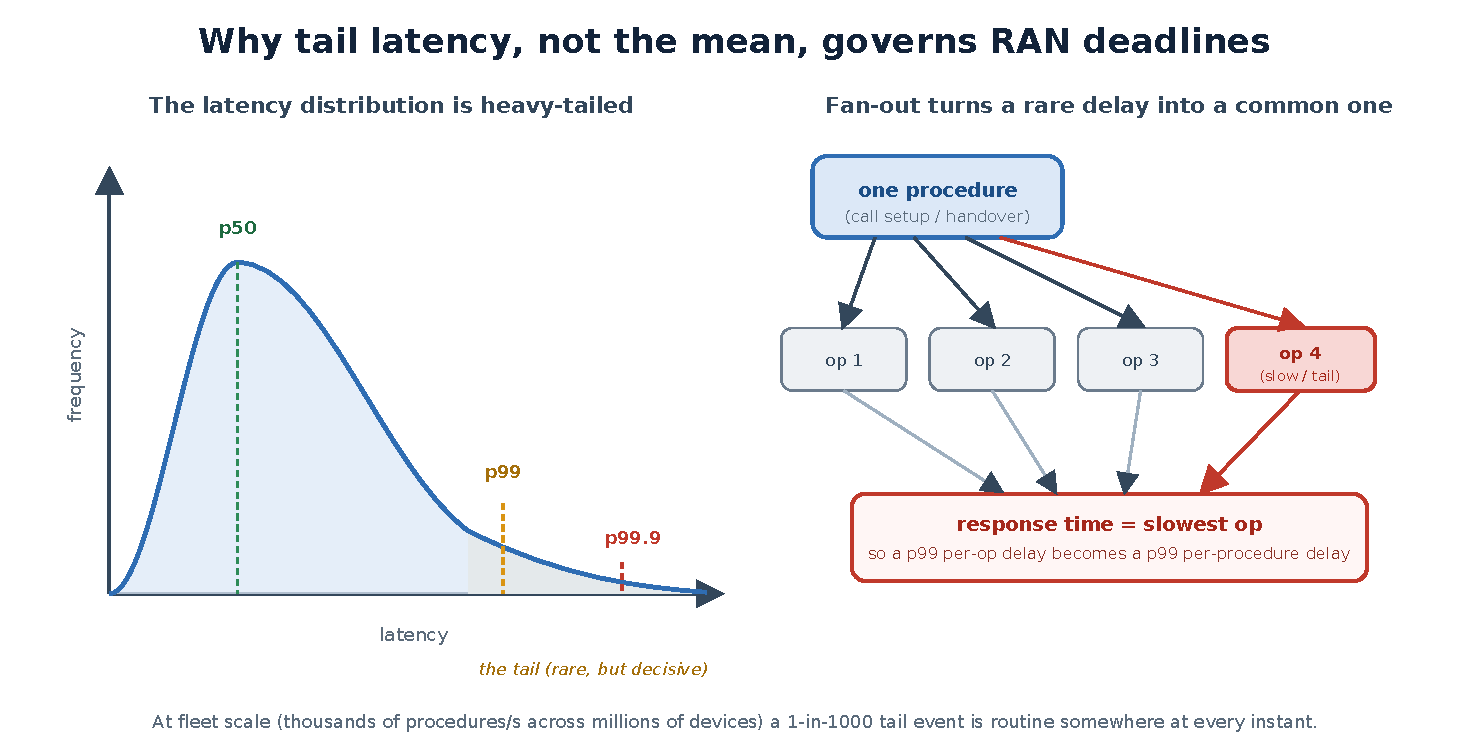
\includegraphics[width=0.78\linewidth]{diagrams/pdf/11_tail_latency_concept.pdf}
\caption[Vì sao đuôi, không phải trung bình, quyết định hạn chót RAN]{Vì sao đuôi, không phải trung bình, quyết định hạn chót RAN. Bên trái, hầu hết thao tác
kết thúc nhanh và một số ít lâu hơn nhiều, nên p99 và p99.9 nằm xa bên phải trung vị. Bên
phải, một thủ tục như thiết lập cuộc gọi chạy nhiều thao tác và chỉ kết thúc khi thao tác
chậm nhất xong, nên trễ chạm một thao tác trong một trăm lần chạm tới phần lớn hơn nhiều của
các thủ tục. Ở quy mô đội tàu, trễ một trong nghìn lần đang xảy ra ở đâu đó mọi
khoảnh khắc.\label{fig:tailconcept}}
\end{figure}

Hệ thống thời gian thực thường được phân cấp theo hệ quả của việc trễ hạn: trong thời gian
thực \emph{cứng} một lần trễ là thất bại, trong thời gian thực \emph{firm} kết quả muộn vô
dụng nhưng không thảm hoạ, và trong thời gian thực \emph{mềm} một lần trễ chỉ làm giảm chất
lượng. Mặt điều khiển RAN nên được xem là thời gian thực mềm đến firm: một phản hồi báo hiệu
trễ thỉnh thoảng làm giảm dịch vụ chứ không gây nguy hiểm, nhưng ở quy mô đội tàu và dưới cơn
bão báo hiệu các suy giảm đó tích lũy thành vấn đề tin cậy toàn mạng. Điều này càng nặng bởi
hành vi hàng đợi: khi tải đưa vào tiến gần công suất phục vụ, trễ hàng đợi tăng mạnh và đuôi
độ trễ bùng nổ gần bão hoà. Mô tả hệ thống do đó cần đẩy tải không chỉ ở mức danh nghĩa mà
\emph{vào quá tải}, đó là lý do phần đánh giá trong luận văn này quét tải lên và vượt điểm
bão hoà.

Đo độ trễ đuôi đúng bản thân nó là cạm bẫy. Một bộ sinh tải vòng kín ngây thơ chờ mỗi phản hồi
trước khi phát yêu cầu tiếp theo mắc \emph{coordinated omission}: khi hệ thống đứng, bộ sinh
cũng đứng theo và đơn giản không ghi các yêu cầu lẽ ra đã tới trong lúc đứng, che có hệ thống
chính xác cái đuôi mà nó phải lộ ra. Hình~\ref{fig:coord} đối chiếu hai mô hình bộ sinh.
Phân biệt bên dưới là mô hình hoá, không phải chi tiết hiện thực. Trong hệ kín một yêu cầu mới
chỉ kích hoạt khi yêu cầu trước hoàn thành, trong khi hệ mở các lần đến độc lập với hoàn thành,
và hai mô hình cho hành vi thời gian phản hồi khác hệ thống trên cùng quy trình phục vụ, với
mô hình kín báo cáo con số thấp hơn~\cite{schroeder2006openclosed}. Đo lường đúng do đó cần mô
hình vòng mở với lịch dự định, hiệu chỉnh coordinated omission, histogram độ trễ độ phân giải
cao giữ độ chi tiết qua nhiều bậc độ lớn, và báo cáo thống kê chặt với lần chạy lặp và khoảng
tin cậy thay vì ước lượng điểm
đơn~\cite{georges2007rigorous}. Các kỹ thuật này được áp dụng ở
Chương~\ref{chapter:eval}.

\begin{figure}[ht]
\centering
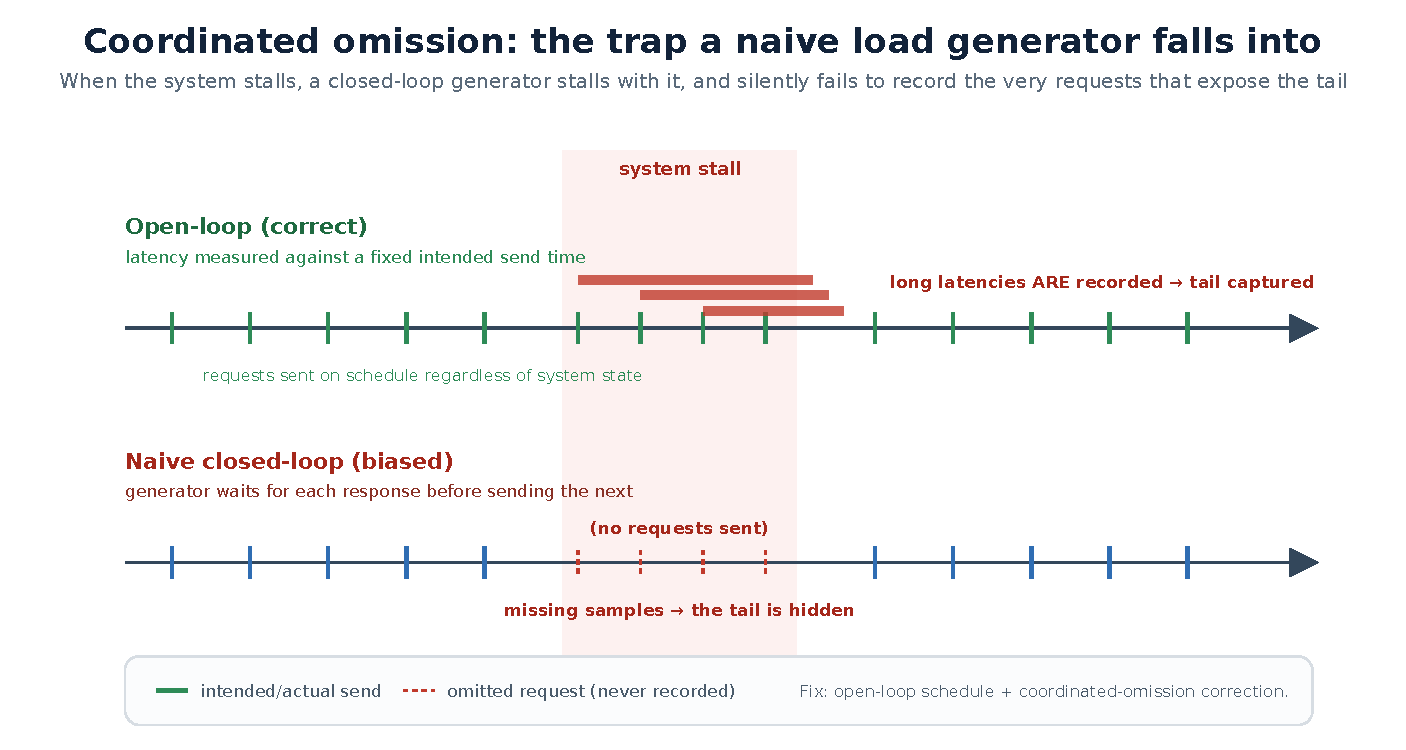
\includegraphics[width=0.78\linewidth]{diagrams/pdf/16_coordinated_omission.pdf}
\caption[Coordinated omission dưới tải vòng mở và vòng kín]{Coordinated omission. Bộ sinh vòng mở phía trên gửi theo lịch cố định ngay cả khi hệ thống
đứng, và tính thời gian mỗi yêu cầu từ lúc đến hạn, nên yêu cầu bị kẹt được ghi với toàn bộ
trễ và đuôi hiện ra. Bộ sinh vòng kín phía dưới chỉ gửi yêu cầu tiếp theo sau khi phản hồi
trước tới. Khi hệ thống đứng nó cũng ngừng gửi, nên các yêu cầu chậm nhất không bao giờ được
phát và không bao giờ được đo, và đuôi biến mất khỏi dữ
liệu.\label{fig:coord}}
\end{figure}

\section{C++ cho hệ thống nhạy độ trễ}\label{sec:cpplatency}
C++ là ngôn ngữ mặc định cho phần mềm mặt điều khiển RAN vì lý do chính đáng. Nó mang trừu
tượng không chi phí, kiểm soát trực tiếp bố cục và cấp phát bộ nhớ, hủy xác định qua idiom
Resource Acquisition Is Initialization (RAII), và trình biên dịch, thư viện cùng công cụ phân
tích trưởng thành, tất cả không có bộ thu gom rác có thể chèn khoảng dừng khó đoán. C++ hiện
đại (C++11 trở đi) thêm con trỏ thông minh (\texttt{std::unique\_ptr}, \texttt{std::shared\_ptr})
tự động hoá sở hữu, ngữ nghĩa move tránh sao chép thừa, và mô hình bộ nhớ chính thức với
\texttt{std::atomic} cho tương tranh có khóa và không khóa. Các tính năng này cho phép viết mã
hệ thống nhanh và, với kỷ luật, tương đối an toàn.

Khó khăn là trình biên dịch không thực thi an toàn này. Lập trình viên mới thực thi. RAII và
con trỏ thông minh giảm lỗi vòng đời mà không loại bỏ hết. Con trỏ hoặc tham chiếu thô có thể
sống lâu hơn đối tượng trỏ tới, biến đổi container có thể vô hiệu iterator, đối tượng có thể
bị dùng sau khi đã move, và không gì trong hệ kiểu ngăn đối tượng mutable được chia sẻ và ghi
bởi nhiều luồng cùng lúc. Kết quả là danh mục lỗi quen thuộc, use-after-free, double-free, tràn
bộ đệm, tranh chấp dữ liệu, deadlock và vô hiệu iterator, dễ đưa vào và tốn kém để tìm ở quy
mô viễn thông. Lỗi hỏng bộ nhớ loại này là vấn đề bảo mật dai dẳng hàng thập kỷ, và các giảm
thiểu triển khai vẫn chỉ là phòng thủ một
phần~\cite{szekeres2013sok}. Mức độ phổ biến được ghi nhận rõ trong công nghiệp. Vấn đề an toàn
bộ nhớ chiếm khoảng 70\,\% lỗ hổng bảo mật Microsoft
báo cáo~\cite{msrc2019memory}, và Google báo cáo giảm mạnh lỗ hổng loại này khi ngôn ngữ an
toàn bộ nhớ được áp dụng trên Android, xuống dưới một phần năm tổng lỗ hổng nền tảng đó vào
năm 2025~\cite{google2022android,vanderstoep2025android}. Danh mục cụ thể này được phát triển
chi tiết ở Chương~\ref{chapter:context} và là cơ sở cho nghiên cứu tiêm lỗi ở
Chương~\ref{chapter:eval}.

Thực hành C++ giảm thiểu các lỗi này bằng công cụ thay vì đảm bảo ngôn ngữ, và công cụ vốn
dĩ chỉ một phần. Bộ dò lỗi động như AddressSanitizer (ASan), ThreadSanitizer (TSan) và
UndefinedBehaviorSanitizer phát hiện nhiều lỗi, nhưng chỉ trên đường mã mà kiểm thử cụ thể
thực sự chạy với đầu vào đúng, và chúng đặt chi phí chạy và bộ nhớ khiến chúng không phù hợp
sản xuất. TSan đặc biệt chỉ báo cáo tranh chấp dữ liệu xảy ra trong một lần chạy, nên tranh
chấp chỉ lộ dưới xen kẽ hiếm có thể lọt. Bộ phát hiện deadlock của nó thừa hưởng giới hạn đó
từ kỹ thuật nó hiện thực, suy luận tiềm năng deadlock từ đồ thị khóa của một trace
đơn~\cite{bensalem2005deadlock}, và nó được phát hành như thành phần thử nghiệm chỉ bao họ
mutex POSIX~\cite{tsandeadlock}. Phân tích tĩnh giúp nhưng mắc false negative và không lý
giải toàn chương trình. Phát hiện do đó là nỗ lực tốt nhất và sau sự kiện, đúng tình huống mà
ngôn ngữ có đảm bảo lúc biên dịch nhằm thay đổi.

Điều đó mô tả C++ như có thể triển khai hôm nay, và ngôn ngữ không đứng yên. Từ năm 2023 ủy
ban tiêu chuẩn theo đuổi \emph{profiles}: tập quy tắc đặt tên bao phủ an toàn kiểu, biên, vòng
đời và số học mà triển khai tuân thủ phải thực thi ở mọi nơi được
bật~\cite{sutter2025profiles}. Hướng đó được chọn thay vì \emph{Safe C++}, đề xuất tập con an
toàn với kiểm tra mượn và thư viện chuẩn riêng, tức mô hình Rust diễn đạt trong
C++~\cite{baxter2024safecpp}. Phép so sánh ở đây vẫn giữ hiệu lực. Profiles chưa được chuẩn
hoá, và tháng 1 năm 2026 chính tác giả vẫn kêu gọi hiện thực và coi thiết kế các profile ban
đầu là việc còn phải
làm~\cite{vandevoorde2026profiles}. Profile tương tranh, cái liên quan các lớp lỗi được liệt kê
ở Chương~\ref{chapter:context}, được đặt sau tập ban đầu và không nằm trong đó: ``cần định
nghĩa và hiện thực thêm profile, đặc biệt một profile
tương tranh''~\cite{vandevoorde2026profiles}. Quy tắc chỉ thực thi khi bật cũng là thứ khác
với thuộc tính hệ kiểu mang vô điều kiện, nhất là khi thực thi là kiểm tra chạy chứ không phải
từ chối biên dịch. Các bản hiện thực so sánh ở đây do đó được xây theo C++23 như đã đặc tả và
phát hành, và Mục~\ref{sec:threats} ghi điều đó ghim phép so sánh vào đâu.

\section{Mô hình sở hữu và an toàn của Rust}
Rust thực thi an toàn bộ nhớ và không tranh chấp dữ liệu lúc biên dịch qua mô hình sở hữu và
mượn~\cite{klabnik2023rust}, và đi kèm công cụ hiện đại trong Cargo cùng kiểm thử tích hợp. Hệ
kiểu cấm tĩnh biến đổi trạng thái chia sẻ và giam các ngoại lệ không tránh khỏi vào mã
\texttt{unsafe} giữ sau API an toàn~\cite{jung2021safe}.

Các đảm bảo này dựa trên hơn khẳng định. Tính đúng đắn của mảnh an toàn của ngôn ngữ, gồm vai
trò \texttt{unsafe} như lối thoát được đánh dấu rõ, đã được thiết lập chính thức bởi dự án
RustBelt~\cite{jung2018rustbelt}, và kỷ luật alias mà ngay cả mã \texttt{unsafe} phải tuân theo
đã được cho ngữ nghĩa vận hành
chính xác~\cite{jung2020stacked}. Bằng chứng thực nghiệm ủng hộ mô hình trong thực tế: trong
mã nguồn thật \texttt{unsafe} được dùng tiết kiệm và cục
bộ~\cite{qin2020rust,astrauskas2020unsafe}, và nghiên cứu mọi CVE an toàn bộ nhớ Rust tìm thấy
mỗi CVE trừ một lỗi trình biên dịch đều liên quan mã
\texttt{unsafe}~\cite{xu2021rustcve}. Lưu ý là không an toàn lan qua phụ thuộc. Ít hơn một phần
ba thư viện dùng \texttt{unsafe} trực tiếp, nhưng phần lớn hơn nhiều không thể kiểm tra tĩnh
đầy đủ vì nó ẩn đâu đó trong chuỗi
gọi~\cite{evans2020rust}, đó là lập luận thêm để giữ lõi an toàn quan trọng của phân hệ không
cần \texttt{unsafe}, như luận văn này làm.

Một thuộc tính quan trọng nhất trong bối cảnh nhạy độ trễ. An toàn này đến từ hệ kiểu và bộ
kiểm tra mượn, không từ công cụ chạy, và được dự định là \emph{không chi phí}. Nghiên cứu hệ
thống lập luận Rust đạt an toàn không chi phí thu gom rác hay kiểm tra chạy, và còn cho phép
kỹ thuật hiệu quả khó trong
C~\cite{balasubramanian2017rust}. Liệu tuyên bố không chi phí có đúng với khối lượng mặt điều
khiển viễn thông chính là thuộc tính mà luận văn này đánh giá.

Cụ thể, bộ kiểm tra mượn từ chối lúc biên dịch chính use-after-free phác thảo ở phần giới
thiệu: chương trình giải phóng ngữ cảnh trong khi tham chiếu tới nó vẫn còn sống thì không
build. Hình~\ref{fig:borrowuaf} đặt lỗi đó ở dạng Quản lý Ngữ cảnh UE cạnh bản C++, biên dịch
và chỉ bị bắt, nếu có, lúc chạy.

\begin{figure}[ht]
\centering
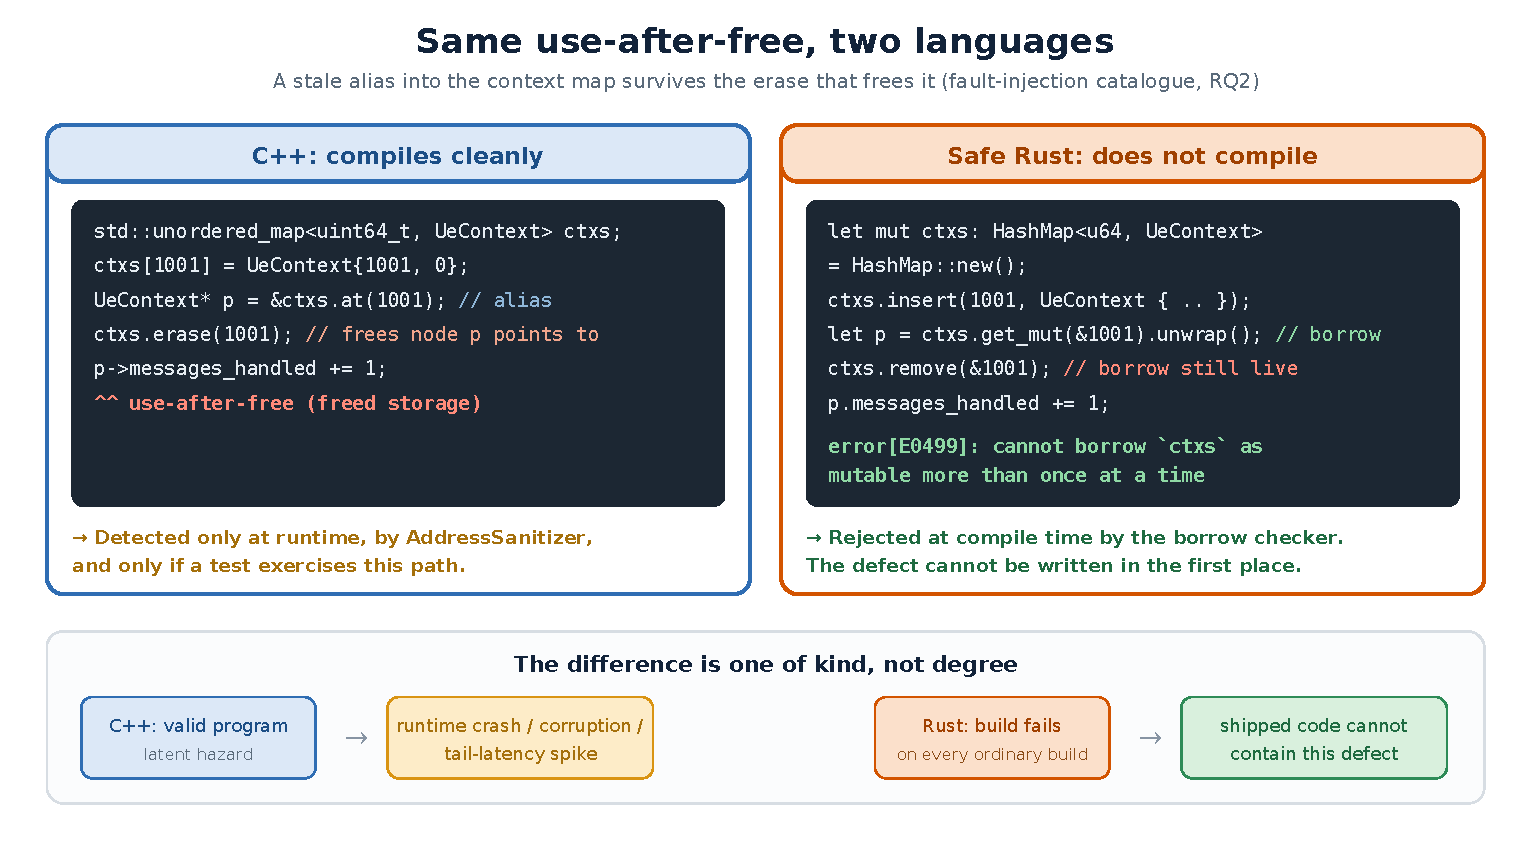
\includegraphics[width=0.78\linewidth]{diagrams/pdf/08_borrow_checker_uaf.pdf}
\caption[Cùng use-after-free trong C++ và Rust an toàn]{Cùng lỗi use-after-free trong C++ và Rust an toàn. Alias cũ vào bản đồ ngữ cảnh sống
sót sau \texttt{erase}/\texttt{remove} giải phóng nó: trong C++ mã này biên dịch và chỉ bị
bắt lúc chạy (và chỉ dưới AddressSanitizer, trên đường mà kiểm thử chạy), trong khi Rust an
toàn bộ kiểm tra mượn từ chối lúc biên dịch (\texttt{E0499}), nên lỗi không thể viết ra. Khác
biệt là về loại, không phải mức độ.\label{fig:borrowuaf}}
\end{figure}

Cùng kỷ luật mở rộng sang tương tranh. Rust mã hoá an toàn luồng trong hệ kiểu qua marker trait
\texttt{Send} và \texttt{Sync}: giá trị chỉ qua ranh giới luồng nếu kiểu là \texttt{Send}, và
chỉ chia sẻ bằng tham chiếu qua luồng nếu là \texttt{Sync}. Chia sẻ giá trị cho phép biến đổi
không đồng bộ do đó là lỗi biên dịch, không phải tranh chấp tiềm ẩn. Đây là thuộc tính Rust
quảng bá là ``fearless concurrency.'' Xử lý lỗi cũng tường minh: thao tác có thể thất bại trả
về giá trị \texttt{Result} mà người gọi phải xử lý, thay vì ném ngoại lệ làm unwind qua luồng
điều khiển ẩn. Cả chi phí lẫn luồng điều khiển của đường thất bại do đó vẫn nhìn thấy được,
đó là lợi thế trong mã nhạy độ trễ nơi bất ngờ ở đuôi mới quan trọng.

Rust không phải ngôn ngữ an toàn bộ nhớ duy nhất, và lý do phép so sánh ở đây vẽ với C++ thay
vì với runtime có quản lý thuộc cùng mô hình này. Java, C\# và Go đạt an toàn bộ nhớ qua runtime
và thu gom rác, đánh đổi xuất sắc cho nhiều phần mềm và kém cho mặt điều khiển nhạy độ trễ đuôi:
khoảng dừng thu gom là nguồn độ trễ đuôi được công nhận trong hệ thống
lớn~\cite{dean2013tail}, và runtime có quản lý từ bỏ kiểm soát bố cục bộ nhớ và lập lịch mà
miền này dựa vào. C, ở cực kia, không an toàn bộ nhớ như C++ trong khi ít trừu tượng hơn để
xây hệ thống lớn. Rust là ngôn ngữ được hỗ trợ rộng đầu tiên kết hợp an toàn bộ nhớ và luồng
lúc biên dịch với không có bộ thu gom rác và thông lượng cùng bộ nhớ cạnh C và
C++~\cite{balasubramanian2017rust,jung2021safe,bugden2022rust}. Đó là lý do ngôn ngữ có quản lý
nằm ngoài phạm vi và lý do phép so sánh có ý nghĩa cho phần mềm mặt điều khiển RAN là C++ với
Rust.

Bảng~\ref{tab:langmodel} đặt cơ chế hai ngôn ngữ cạnh nhau. Phân biệt nó xây quanh không phải
mối nguy mỗi ngôn ngữ gọi tên gì, vì cả hai gọi tên gần giống nhau, mà \emph{khi nào} và \emph{bởi
cái gì} mỗi thứ bị loại trừ, và hai hàng cuối đánh dấu nơi câu trả lời không còn là ``bởi
trình biên dịch'' với cả hai.

\begin{table}[H]
\centering
\small
\caption[Cách mỗi ngôn ngữ thực thi các thuộc tính được đo]{Cách mỗi ngôn ngữ thực thi các thuộc tính mà luận văn này đo. Các hàng trên quy
tắc là nơi hai ngôn ngữ khác về loại chứ không chỉ mức độ: trình biên dịch từ chối chương trình
loại trừ lỗi khỏi mọi lần thực thi, trong khi bộ dò lỗi chỉ loại trừ khỏi các lần thực thi mà
kiểm thử có công cụ tình cờ chạy. Các hàng dưới quy tắc là ranh giới phát triển ở
Chương~\ref{chapter:context} và đo ở Chương~\ref{chapter:eval}, nơi không ngôn ngữ nào có đảm
bảo tĩnh.\label{tab:langmodel}}
\renewcommand{\arraystretch}{1.2}
\begin{tabular}{@{}R{0.20\linewidth} R{0.36\linewidth} R{0.36\linewidth}@{}}
\hline\hline
Khía cạnh & C++ hiện đại & Rust \\
\hline
Vòng đời đối tượng & RAII và con trỏ thông minh, áp dụng theo quy ước. Con trỏ hoặc tham chiếu thô có thể sống lâu hơn đối tượng trỏ tới & Sở hữu: mỗi giá trị có một chủ sở hữu và bị giải phóng đúng một lần \\
Alias & Không hạn chế: bất kỳ số alias mutable nào cũng có thể cùng tồn tại & Mượn: hoặc một tham chiếu mutable hoặc nhiều tham chiếu chia sẻ, không bao giờ cả hai \\
Biên & Không kiểm tra trên \texttt{operator[]}, chỉ kiểm tra qua \texttt{at()} & Kiểm tra mặc định, bỏ qua nơi chỉ số chứng minh được trong phạm vi \\
An toàn luồng & Không diễn đạt trong hệ kiểu: chia sẻ đối tượng mutable qua luồng vẫn biên dịch & Marker trait \texttt{Send} và \texttt{Sync}. Chia sẻ không đồng bộ là lỗi kiểu \\
Báo hiệu lỗi & Ngoại lệ hoặc mã lỗi: đường thất bại có thể vô hình tại điểm gọi & Giá trị \texttt{Result} người gọi phải xử lý. Đường thất bại tường minh \\
Lối thoát & Toàn bộ ngôn ngữ & Khối \texttt{unsafe}, có giới hạn và đếm được cơ học \\
Giai đoạn phát hiện & Chạy, dưới bộ dò lỗi đúng, trên đường kiểm thử chạy & Biên dịch, trên mọi build thường, bất kể độ phủ kiểm thử \\
\hline
Thứ tự khóa & Không kiểm tra & Không kiểm tra \\
Tính nguyên tử của thao tác ghép & Không kiểm tra & Không kiểm tra \\
\hline
\end{tabular}
\end{table}

\section{Mô hình tương tranh cho phần mềm mặt điều khiển}
Cách cấu trúc tương tranh định hình cả tính đúng đắn lẫn độ trễ đuôi. Mô hình chi phối là
tương tranh \emph{bộ nhớ chia sẻ}, trong đó luồng biến đổi trạng thái chung được bảo vệ bởi
mutex và atomic. Nó linh hoạt, nhưng là nguồn tranh chấp, deadlock, tranh chấp khóa và đảo
ngược ưu tiên, và trường hợp xấu nhất khó giới hạn. Phương án thay thế là tương tranh
\emph{truyền thông} hoặc \emph{không chia sẻ}, trong đó trạng thái được phân vùng để mỗi phần
do một luồng sở hữu và mọi tương tác qua thông điệp, như mô hình actor. Nó đổi linh hoạt lấy
khả năng mở rộng và lý luận đơn giản hơn nhiều, và ánh xạ tự nhiên lên phân vùng theo UE, vì
trạng thái mỗi UE phần lớn độc lập. Lựa chọn cũng dịch chuyển đại lượng đo ở đây: cấu trúc
một luồng mỗi lõi tự thay đổi độ trễ đuôi ứng
dụng~\cite{enberg2019threadpercore}, nên mô hình được giữ cố định giữa hai bản hiện thực thay
vì giao cho idiom mỗi ngôn ngữ. Hình~\ref{fig:concmodels} đối chiếu hai mô hình.

\begin{figure}[ht]
\centering
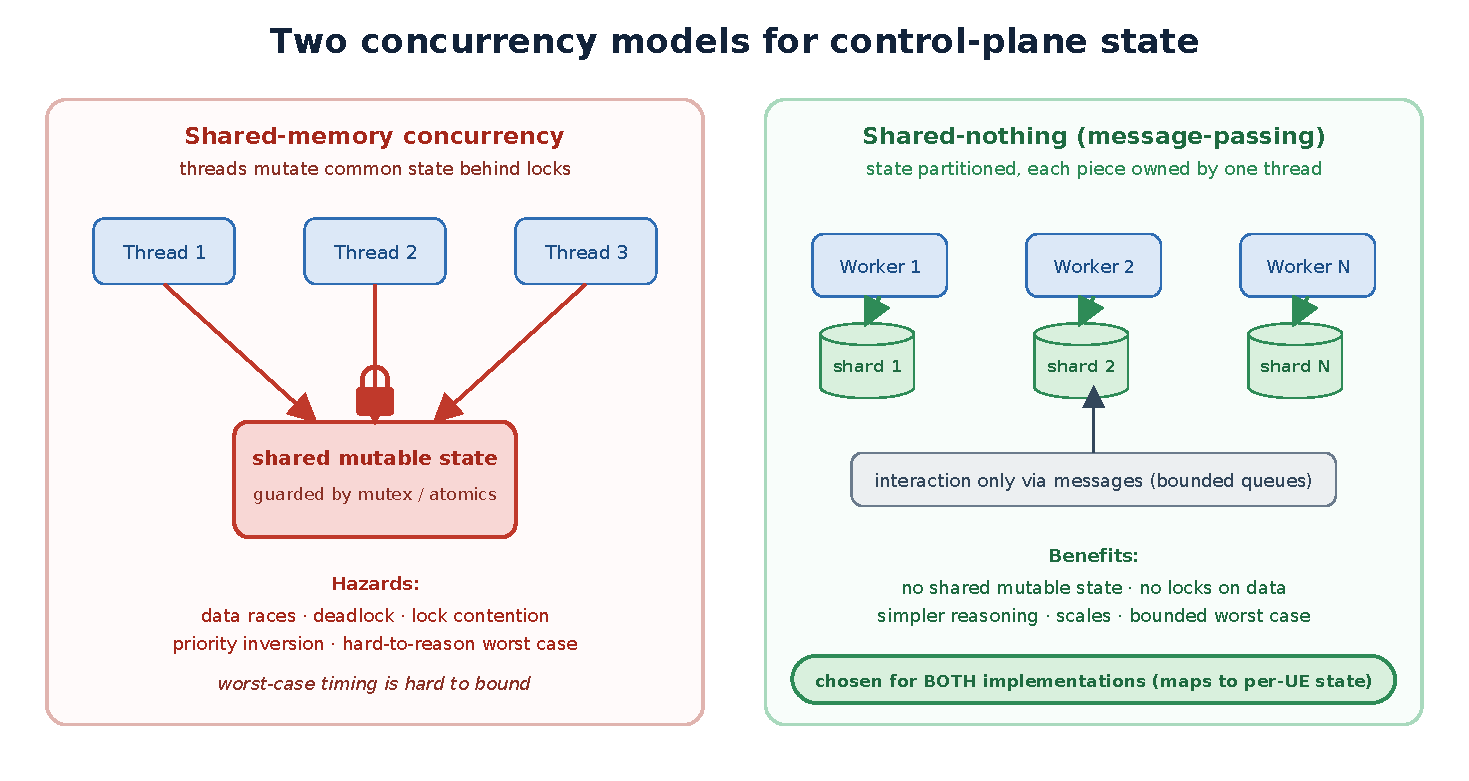
\includegraphics[width=0.78\linewidth]{diagrams/pdf/12_concurrency_models.pdf}
\caption[Hai mô hình tương tranh cho trạng thái mặt điều khiển]{Hai mô hình tương tranh cho trạng thái mặt điều khiển. Tương tranh bộ nhớ chia sẻ (trái)
cho luồng biến đổi trạng thái chung sau khóa và là nguồn tranh chấp dữ liệu, deadlock và tranh
chấp khóa, với trường hợp xấu nhất khó giới hạn. Truyền thông không chia sẻ (phải) phân vùng
trạng thái để mỗi shard do một worker sở hữu và mọi tương tác qua hàng đợi có giới hạn, loại
khóa trên dữ liệu ngữ cảnh và ánh xạ lên phân vùng theo UE. Đây là mô hình hai bản hiện thực
áp dụng.\label{fig:concmodels}}
\end{figure}

Cấu trúc thứ ba, runtime bất đồng bộ trên bộ lập lịch work-stealing, là idiom trong cả hai
ngôn ngữ và không được dùng trong cả hai. Hành vi thời gian của nó thuộc runtime, không thuộc
ngôn ngữ chứa nó: nghiên cứu thời gian thực về Rust bất đồng bộ tìm một ứng dụng đáp ứng hoặc
trễ hạn tùy runtime và ánh xạ ưu tiên luồng, và cấu hình đáp ứng hạn không phải cấu hình
work-stealing
thông thường~\cite{skoudlil2025asyncrust}. Áp dụng runtime như vậy sẽ nhập biến thiên mà nghiên
cứu này tồn tại để loại trừ, và Mục~\ref{sec:relatedwork} quay lại phép so sánh mà nó không bị
loại trừ.

Hàng đợi giữa nhà sản xuất và người tiêu thụ là lựa chọn thứ hai, độc lập. Hàng đợi không giới
hạn che quá tải và để độ trễ cùng bộ nhớ tăng không giới hạn. Hàng đợi \emph{có giới hạn}, dù
chặn để backpressure hay loại bỏ, giới hạn bộ nhớ trường hợp xấu nhất và làm quá tải nhìn thấy
được, điều độ trễ đuôi dự đoán được đòi hỏi. Cả hai lựa chọn cố định kiến trúc mà hai bản hiện
thực dùng ở Chương~\ref{chapter:design}: thiết kế không chia sẻ, một luồng mỗi shard, trong đó
trạng thái UE chia thành các lát độc lập gọi là \emph{shard}, mỗi lát do đúng một luồng worker
sở hữu, nên không hai luồng chạm cùng ngữ cảnh. Yêu cầu tới shard qua hàng đợi đa nhà sản xuất,
một người tiêu thụ có giới hạn chặn khi đầy.

\section{Khả năng tương tác giữa C++ và Rust}\label{sec:interop}
Áp dụng ngôn ngữ mới trong hệ thống lớn sẵn có buộc phải tăng dần: thành phần Rust phải cùng
tồn tại và được gọi từ mã nguồn C++ đáng kể. Mẫu số chung cho việc đó là giao diện nhị phân
ứng dụng C (ABI). Rust có thể lộ hàm với liên kết \texttt{extern "C"} và đưa ra \emph{handle
mờ} tới đối tượng do Rust sở hữu, mà C++ gọi qua header C. Công cụ tự động hoá một phần:
\texttt{bindgen} (binding Rust từ header C), \texttt{cbindgen} (header C từ Rust), và crate
\texttt{cxx} (cầu hai chiều an toàn hơn). Tương tác không miễn phí. Vượt ranh giới bước ra ngoài
ngôn ngữ được kiểm tra, nên đường ghép phải chứa mã \texttt{unsafe}, giá trị phức tạp hơn đơn
giản nhất cần marshalling, và giao diện ngoại phải được thiết kế có chủ đích. Kích thước đường
ghép, \texttt{unsafe} nó tập trung, và chi phí vượt ranh giới mỗi lần gọi là đại lượng RQ4 đo
ở Chương~\ref{chapter:eval}.

Một phân biệt giới hạn những gì các đo lường đó có thể thiết lập. Tập trung \texttt{unsafe} ở
đường ghép nói trình biên dịch kiểm tra gì, không nói gì có thể xảy ra lúc chạy. Thành phần Rust
liên kết vào host C++ chia một không gian địa chỉ với nó, nên lỗi phía C++ có thể hỏng dữ liệu
do Rust sở hữu dù bao nhiêu phía Rust bộ kiểm tra mượn đã xác minh. Điều này đã được chứng minh
thực nghiệm, và biện pháp đề xuất cô lập hai heap trong phần cứng hoặc runtime thay vì tin kỷ
luật giao
diện~\cite{rivera2021galeed,kirth2022pkrusafe}. Các lớp lỗi đặc thù ranh giới Rust/C được liệt
kê tách khỏi lỗi của từng
ngôn ngữ~\cite{li2022crosslang}, và chính bộ sinh binding cũng mang
lỗi~\cite{cai2026interop}. Hệ quả được nêu một lần ở đây và được tôn trọng xuyên suốt: lõi không
cần \texttt{unsafe} có nghĩa lỗi của chính lõi bị loại lúc biên dịch, và không có nghĩa lõi
được bảo vệ khỏi host.

Điều gần đây thay đổi là tầm với của công cụ, không phải đảm bảo. Bộ kiểm tra mô hình không
trạng thái cho Rust giờ khám phá không gian trạng thái chương trình cùng phụ thuộc ngoại, đưa
tranh chấp dữ liệu phát sinh từ tương tác hai ngôn ngữ vào tầm một bộ kiểm tra dù chúng nằm
ngoài những gì bộ kiểm tra mượn
thấy~\cite{pearce2026rustmc}. Khả năng đó tới sau khi nguyên mẫu đo ở đây được xây, và
Chương~\ref{chapter:conclusions} ghi nó là bước tiếp theo cho đường ghép.

\section{Khoảng trống nghiên cứu}\label{sec:gap}
Các mục trước dựng khoảng trống. Mặt điều khiển RAN là miền thời gian thực mềm đến firm, tương
tranh cao, nơi hành vi đuôi khi quá tải, không phải thông lượng trung bình, quyết định chất
lượng mạng giao. C++ cung cấp kiểm soát và hiệu năng miền đòi hỏi, nhưng giao cả lớp lỗi bộ nhớ
và tương tranh cho phát hiện nỗ lực tốt nhất sau sự kiện. Rust hứa ngăn các lớp đó lúc biên
dịch không tốn chi phí chạy, và đưa ra lộ trình áp dụng tăng dần đáng tin qua ABI C.

Miền không phải chưa được nghiên cứu, và khối lượng công trước dễ bị đánh giá thấp vì gần như
không có trong chỉ mục. Ít nhất năm luận văn thạc sĩ do nhà cung cấp lưu trữ, tất cả tại
Ericsson, đã so sánh ngôn ngữ ứng viên cho phần mềm RAN và viễn thông. Một cân chi phí chạy với
hiệu quả phát triển giữa C++, Rust và Go~\cite{karlback2021ran}. Một hỏi Rust có thể thay C
trong quản lý nút RAN~\cite{olsson2023ranmgmt}. Một xây bộ xử lý gói một luồng mỗi lõi trên
Rust bất đồng bộ và đo với ứng dụng DPDK nó sao
chép~\cite{olsson2023asyncpackets}. Một đo trung vị và độ trễ phân vị thứ 99 cho thủ tục mặt
điều khiển qua năm framework lập trình
bất đồng bộ~\cite{arvidsson2025async}. Cuối cùng xây bản C++ và Rust khớp của trình dịch ASN.1
và so sánh thống kê~\cite{emberg2023asn1}. Cả năm đều liên quan trực tiếp, và hai báo cáo khác
biệt bất lợi cho Rust.

Ba trong số đó thay đổi ngôn ngữ cùng runtime và mô hình tương tranh, nên khác biệt đo được
không thể quy cho ngôn ngữ thay vì framework xây trên
nó~\cite{karlback2021ran,olsson2023asyncpackets,arvidsson2025async}. Cỡ hiệu ứng chạm hệ số năm,
đó là dấu hiệu phần lớn đo lường thuộc runtime. Hai còn lại giữ thiết kế gần cố định hơn nhưng
báo cáo thời gian thực thi và bộ nhỉ đỉnh thay vì hành vi đuôi dưới tải tăng~\cite{olsson2023ranmgmt,emberg2023asn1},
và gần nhất, Emberg và Wadsten, đo biến đổi không trạng thái thay vì phân hệ có trạng thái,
tương tranh. Hình~\ref{fig:gapmap} đặt các nghiên cứu lân cận so với các thuộc tính câu trả lời
có kiểm soát cần, và mẫu nó cho thấy mỗi nghiên cứu giữ một số và không nghiên cứu nào giữ
hết.

Sự tập trung bằng chứng đó cũng là một phần khoảng trống. Cả năm nghiên cứu đến từ một nhà cung
cấp, và kết luận của chúng chưa bao giờ được thử với phần mềm, mục tiêu hay quy ước của tổ chức
khác, nên điều biết về câu hỏi này là những gì framework của một công ty báo cáo về nó. Hồ sơ
công bố phía kia trống hơn: không có nghiên cứu Rust trong các ấn phẩm được lập chỉ mục của
nhà cung cấp chủ trì công trình này, và lập trường bạn đồng nghiệm gần nhất từ phía đó lập luận
cho việc làm cho sanitisation lỗi bộ nhớ thực tế thay vì thay nó bằng đảm bảo lúc biên
dịch~\cite{gjomemo2016mesc}, đó là chiến lược luận văn này đối chứng. Mục~\ref{sec:relatedwork}
so sánh năm nghiên cứu với nghiên cứu này trực tiếp.

\begin{figure}[ht]
\centering
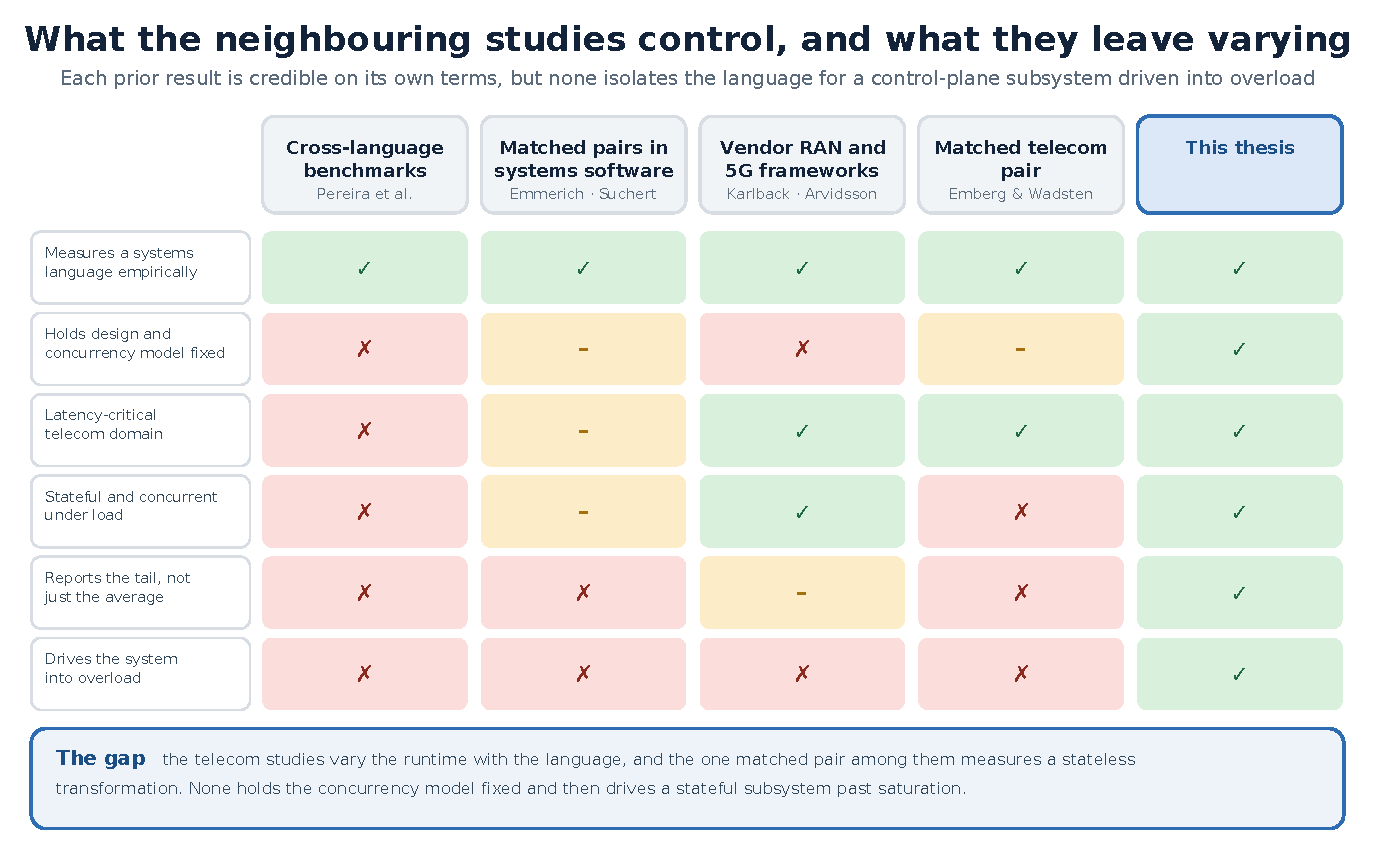
\includegraphics[width=0.78\linewidth]{diagrams/pdf/29_research_gap.pdf}
\caption[Điều các nghiên cứu lân cận kiểm soát và để thay đổi]{Điều các nghiên cứu lân cận kiểm soát và để thay đổi. Mỗi hàng là thuộc tính mà câu
trả lời có kiểm soát cho câu hỏi nghiên cứu cần. Mỗi cột là một nghiên cứu. Các so sánh chéo
ngôn ngữ đo đúng loại đối tượng nhưng sai chế độ, báo cáo trung bình trên khối lượng đa mục
đích. Cặp khớp trong phần mềm hệ thống giữ thiết kế cố định, nhưng ngoài miền này và dưới bão
hoà. Các nghiên cứu framework RAN và 5G của nhà cung cấp chạm đúng miền, và một trong số đó báo
cáo đuôi, nhưng trong tất cả ngôn ngữ thay đổi cùng runtime và mô hình tương tranh. Cặp viễn
thông khớp duy nhất, Emberg và Wadsten, kiểm soát thiết kế nhưng đo biến đổi không trạng thái.
Giữ thiết kế và mô hình tương tranh cố định cho phân hệ có trạng thái, tương tranh rồi đẩy qua
bão hoà là điều luận văn này thêm vào. Đóng góp là kiểm soát, không phải kỹ thuật đo mới.\label{fig:gapmap}}
\end{figure}

Vì vậy điều còn thiếu trong tài liệu là bằng chứng \emph{trực tiếp, có kiểm soát} cho phân hệ
mặt điều khiển đại diện: liệu Rust có thực sự giữ độ trễ đuôi và khả năng dự đoán khi quá tải
so với C++ hiện đại \emph{khi mô hình tương tranh, thuật toán và cấu trúc dữ liệu được giữ
cố định}, chính xác lớp lỗi nào nó loại bỏ và giai đoạn nào phần còn lại bị bắt, mô hình an toàn
tốn bao nhiêu về thông lượng và tài nguyên, và áp dụng tăng dần tốn bao nhiêu trong thực tế.
Lấp khoảng trống này là mục đích của bốn câu hỏi nghiên cứu. Chương tiếp theo neo chúng vào
phân hệ cụ thể, lớp lỗi và thuộc tính thời gian liên quan, và
Chương~\ref{chapter:methodology} nêu phương pháp luận để theo đuổi chúng.

\chapter{Bối cảnh bài toán: Quản lý Ngữ cảnh UE và tính dự đoán được\label{chapter:context}}
\chaptermark{Bối cảnh bài toán}

\section{Phân hệ Quản lý Ngữ cảnh UE}\label{sec:uecm}
Phân hệ được nghiên cứu là một dịch vụ Quản lý Ngữ cảnh UE. Dịch vụ này được mô hình hoá theo
một miền dịch vụ gNB-CU-CP thực tế của Nokia, sở hữu vòng đời ngữ cảnh UE, thực thi thủ tục
RRC~\cite{3gpp38331}, và di động/bàn giao, tức các chức năng mà kiến trúc 3GPP giao cho phần
mặt điều khiển của một gNB phân tách (Mục~\ref{sec:ranarch}).

Hình~\ref{fig:fsm} cho thấy máy trạng thái vòng đời ngữ cảnh UE mà cả hai bản hiện thực mã hoá
giống hệt nhau. Máy trạng thái này chính là thứ mà khối lượng công việc hỗn hợp ở
Mục~\ref{sec:workload} đưa mỗi UE đi qua.

\begin{figure}[ht]
\centering
\begin{tikzpicture}[
    ->, >=Stealth, node distance=3.2cm, font=\small,
    every state/.style={draw, minimum size=1.5cm, fill=blue!6, thick},
    every edge/.style={draw, thick}
  ]
  \node[state, initial, initial text=\scriptsize create] (idle) {Idle};
  \node[state, right=of idle] (conn) {Connected};
  \node[state, right=of conn] (reconf) {Reconf.};
  \node[state, below=1.9cm of conn, fill=gray!10] (rel) {Released};

  \path (idle)  edge node[above,font=\scriptsize]{setup} (conn)
        (conn)  edge[bend left=18] node[above,font=\scriptsize]{begin} (reconf)
        (reconf) edge[bend left=18] node[below,font=\scriptsize]{complete / abort} (conn)
        (conn)  edge node[right,font=\scriptsize,pos=0.45]{release} (rel)
        (idle)  edge[bend right=32] node[below,font=\scriptsize,pos=0.6]{release} (rel);
  \path (conn) edge[loop above] node[font=\scriptsize]{signal / add\_drb} (conn);
\end{tikzpicture}
\caption[Máy trạng thái vòng đời ngữ cảnh UE]{Máy trạng thái vòng đời ngữ cảnh UE. \texttt{create} cấp phát một ngữ cảnh ở
\texttt{Idle} và \texttt{setup} kết nối nó. \texttt{signal} và \texttt{add\_drb} được xử lý tại
chỗ khi ở \texttt{Connected}. Một tái cấu hình hoặc bàn giao đi qua \texttt{Reconfiguring} rồi
trở lại khi \texttt{complete} hoặc \texttt{abort}, còn \texttt{release} tháo dỡ ngữ cảnh. Thao
tác không hợp lệ với trạng thái hiện tại trả về \texttt{OpError} thay vì đổi trạng thái.\label{fig:fsm}}
\end{figure}

\paragraph{Vì sao chọn phân hệ này.}
UECM phù hợp làm đối tượng nghiên cứu vì vừa đại diện vừa đủ nhỏ để kiểm soát. Đây là chức năng
lớp~3 RAN cốt lõi, và mang các thuộc tính khiến mã mặt điều khiển sản xuất khó xử lý: trạng thái
có thể thay đổi theo từng UE, vòng đời thao tác chặt chẽ, mức độ đồng thời cao giữa các UE, cùng
mục tiêu độ trễ và độ tin cậy mà hệ thống 5G đặt ra cho thủ tục mặt điều
khiển~\cite{3gpp38913,3gpp22261}. Kết luận về cách một ngôn ngữ xử lý các thuộc tính đó do đó
chuyển được sang các dịch vụ mặt điều khiển có trạng thái và đồng thời khác. Phân hệ cũng đủ
nhỏ để đặc tả chính xác, hiện thực trung thực bằng hai ngôn ngữ, và suy luận trọn vẹn, tức điều
kiện tiên quyết để so sánh có kiểm thử tương đương trở nên khả thi. Một phân hệ lớn hơn sẽ đổi
lấy tính ngoại hiệu bằng tính nội hiệu mà một so sánh ngôn ngữ công bằng phụ thuộc vào. UECM
nằm ở điểm cả hai vẫn trong tầm với.

\paragraph{Tập thao tác.}
Giao diện mà nghiên cứu khai thác cố ý nhỏ và theo hướng vòng đời. Nó có thể tạo và giải phóng
một ngữ cảnh, thiết lập kết nối (\texttt{Idle}$\rightarrow$\texttt{Connected}), xử lý một thông
điệp báo hiệu trong phiên, thêm một data radio bearer, bắt đầu, hoàn tất hoặc huỷ một tái cấu
hình hoặc bàn giao, và tra cứu trạng thái ngữ cảnh dưới tải đồng thời. Mỗi thao tác được định
nghĩa cho mọi trạng thái của máy ở Hình~\ref{fig:fsm}: thao tác bất hợp pháp ở trạng thái hiện
tại trả về lỗi có kiểu và giữ nguyên ngữ cảnh, thay vì ném ngoại lệ hoặc làm hỏng trạng thái.
Tập thao tác kín và có kiểu này là điều cho phép cùng một bộ vectơ kiểm thử và cùng khối lượng
công việc dẫn cả hai bản hiện thực theo các đường đi giống hệt nhau (Mục~\ref{sec:parity}).

\section{Các lớp lỗi an toàn bộ nhớ và đồng thời}\label{sec:defects}
Các lỗi ảnh hưởng tới mã mặt điều khiển C++ loại này chia thành hai họ. Họ \emph{an toàn bộ
nhớ} liên quan tới vòng đời và biên của đối tượng: \emph{use-after-free} truy cập vùng nhớ đã
được giải phóng, \emph{double-free} giải phóng cùng một vùng hai lần, và \emph{buffer overflow}
đọc hoặc ghi vượt cuối vùng cấp phát. Họ \emph{đồng thời} liên quan tới truy cập không đồng bộ
hoặc sai thứ tự từ nhiều luồng: \emph{data race} là một cặp truy cập không đồng bộ vào cùng vị
trí mà ít nhất một bên là ghi, \emph{deadlock} là chờ khoá vòng, còn \emph{iterator invalidation}
là dùng iterator hoặc tham chiếu vào container sau khi một thay đổi đã di chuyển hoặc giải phóng
vùng nhớ bên dưới. Điểm chung là trong C++ chúng đều \emph{im lặng}: trình biên dịch chấp nhận
từng lớp, và trên các đường đi mà kiểm thử thông thường tình cờ chạm tới, chúng có thể trông
như hoạt động đúng, chỉ lộ ra sau dưới dạng hỏng dữ liệu, sập chương trình, hoặc đột biến độ trễ
không dự đoán được. Đây là cùng các lớp hỏng bộ nhớ mà hàng thập kỷ nghiên cứu bảo mật vẫn khó
kìm hãm trong C và C++~\cite{szekeres2013sok}.

Mỗi lớp có một hiện thân tự nhiên trong Quản lý Ngữ cảnh UE, đó là lý do phân hệ phù hợp để
nghiên cứu chúng:

\begin{itemize}
  \item \textbf{Use-after-free.} Một thông điệp báo hiệu giữ con trỏ thô hoặc tham chiếu tới
        ngữ cảnh UE mà một \texttt{release} đồng thời đã xoá khỏi bản đồ ngữ cảnh. Bộ xử lý
        đang bay khi đó giải tham chiếu vùng nhớ đã giải phóng.
  \item \textbf{Double-free.} Đường \texttt{release} chạy hai lần cho cùng một UE, ví dụ vì
        \texttt{release} được truyền lại không được làm bất biến, giải phóng tài nguyên sở hữu
        của ngữ cảnh lần thứ hai.
  \item \textbf{Iterator invalidation.} Mã lặp danh sách data radio bearer của ngữ cảnh trong khi
        thêm hoặc gỡ bearer, nên iterator trỏ vào vùng nhớ mà container đã tái cấp phát.
  \item \textbf{Data race.} Hai worker cập nhật cùng một trường ngữ cảnh, bộ đếm hoạt động hoặc
        cờ trạng thái, mà không đồng bộ hoá, nên các truy cập tranh chấp.
  \item \textbf{Unguarded shared mutation.} Một ngữ cảnh được chia sẻ bằng tham chiếu giữa các
        luồng và bị thay đổi mà không có khoá hay kỷ luật khác, một race mà nguyên nhân gốc là
        không có quy tắc sở hữu cho trạng thái dùng chung.
  \item \textbf{Use-after-move.} Thủ tục nhận di chuyển ngữ cảnh vừa dựng vào kho và rồi trả lời
        yêu cầu từ biến cục bộ vừa bị move khỏi, nên phản hồi mang danh tính rỗng. Lớp này được
        giữ vì công cụ C++ \emph{không} nói gì về nó. Không có gì bị hỏng và không có hành vi
        không xác định, vì đối tượng đã move vẫn ở trạng thái hợp lệ nhưng không xác định, nên
        lỗi không có triệu chứng lúc chạy để sanitiser bắt.
  \item \textbf{Thread-unsafe handle shared across workers.} Tay cầm ngữ cảnh đếm tham chiếu mà
        bộ đếm không nguyên tử, thói quen đường nóng chọn khi khối điều khiển nguyên tử của con
        trỏ chia sẻ tốn hơn lợi ích, được truyền cho hai shard worker. Ràng buộc khiến tay cầm
        đúng được viết trong comment, vì C++ không có cách diễn đạt gắn kết luồng trong kiểu.
\end{itemize}

Bảy lớp này nằm gọn trong các bảo đảm mà Rust tuyên bố, nên chúng là thử nghiệm tự nhiên xem
tuyên bố đó có đứng không. Tuy nhiên chỉ kiểm thử chúng sẽ khắc sẵn câu trả lời mong đợi vào
lựa chọn ca kiểm thử, nên thêm bảy lớp nữa được đưa vào nghiên cứu vì lý do ngược lại, tức có cơ
sở kỳ vọng Rust an toàn \emph{không} ngăn được chúng:

\begin{itemize}
  \item \textbf{Lock-order deadlock.} Một bàn giao khoá ngữ cảnh UE nguồn rồi đích, trong khi
        bàn giao đồng thời chiều ngược khoá đích rồi nguồn, và hai bên chờ nhau vô hạn. Không có
        gì vi phạm vòng đời đối tượng hay aliasing. Lỗi nằm ở thứ tự lấy khoá.
  \item \textbf{Lost update.} Hai worker tăng bộ đếm hoạt động của ngữ cảnh qua read-modify-write
        tách thành hai vùng tới hạn riêng. Mỗi truy cập riêng lẻ đều đồng bộ đúng, nên đây là
        \emph{race condition} chứ không phải \emph{data race}: vi phạm nguyên tử nằm ở tổ hợp
        thao tác, không phải ở bản thân truy cập bộ nhớ, và nó làm hỏng giá trị im lặng thay vì
        sập chương trình.
  \item \textbf{Leak through a reference cycle.} Một ngữ cảnh và đối tác bàn giao giữ tham chiếu
        sở hữu lẫn nhau, nên không bộ đếm nào về không và không bên nào bị huỷ. Đếm tham chiếu
        không thu gom chu trình trong cả hai ngôn ngữ, và rò rỉ là an toàn trong Rust theo thiết
        kế tường minh. Đây là phát biểu ranh giới rõ nhất trong danh mục, vì cả hai ngôn ngữ
        thất bại giống nhau.
  \item \textbf{Integer overflow in a release build.} Tính bước TEID của bearer vượt độ rộng
        kiểu. Trong C++ tràn số có dấu là \emph{không xác định}, nên chương trình không có
        nghĩa. Trong Rust nó \emph{được định nghĩa} là quấn vòng, vì hồ sơ \texttt{opt-level~=~2}
        mà nghiên cứu so sánh tắt \texttt{overflow-checks}, nên chương trình có nghĩa và nghĩa
        đó sai. Mẫu không giả định: CVE-2026-64467 trong \texttt{rust\_binder} là lỗi bước cùng
        hình dạng.
  \item \textbf{Worker failure blast radius.} Một shard worker thất bại giữa chừng thủ tục. Mô hình
        đồng thời ở Mục~\ref{sec:concurrency} biến một shard thành miền lỗi theo cấu trúc, và
        không hệ kiểu nào của hai ngôn ngữ buộc nó hành xử như vậy: trong C++ ngoại lệ thoát khỏi
        callable của luồng chấm dứt cả tiến trình, còn trong Rust panic giam trong luồng nhưng
        độc trạng thái nó giữ, nên thiệt hại lan theo dữ liệu. Trực tiếp liên quan tới luận điểm
        tính sẵn sàng cấp nhà mạng, và không gì trong hai hệ kiểu giải quyết.
  \item \textbf{Double-free across the seam.} Máy chủ C++ giữ tay cầm mờ tới ngữ cảnh Rust và
        giải phóng hai lần, tức \texttt{release} truyền lại của lớp double-free ở trên, giờ diễn
        đạt theo cách ranh giới hàm ngoại bắt buộc. Rust an toàn từ chối giải phóng kép vì sở
        hữu theo dõi giá trị. Một đường nối không giữ được điều đó, vì đưa con trỏ thô cho caller
        C chính là thao tác chấm dứt kiến thức của trình biên dịch về nó. Lớp do đó xuất hiện
        hai phía ranh giới, là phát biểu sắc nhất về bản chất ranh giới.
  \item \textbf{Forgotten lock guard.} Thiết lập bearer lấy khoá ngữ cảnh và lỗi kiểm tra khiến
        hàm trả về mà không nhả khoá, nên worker kế tiếp chạm ngữ cảnh đó chờ vô hạn. Rust loại
        dạng thường gặp của lỗi này, vì guard nhả khi bị drop và không có unlock viết tay để bỏ
        qua. Nó không loại bỏ lỗi, vì guard là một giá trị và rò rỉ giá trị là an toàn. Nơi chu
        trình tham chiếu rò bộ nhớ, đây rò chính ngữ cảnh.
\end{itemize}

Cùng nhau mười bốn lớp này tạo danh mục được tiêm ở Chương~\ref{chapter:eval}, và sự tách hai
nhóm là điều cho phép nghiên cứu báo cáo một ranh giới thay vì một phán quyết. Buffer overflow
được mô tả ở trên cho đầy đủ nhưng không được tiêm, vì không bản hiện thực nào làm số học con trỏ
thô trên kho ngữ cảnh, nên một ca tiêm sẽ là cấu trúc giả tạo chứ không phải lỗi hợp lý trong
phân hệ này. Bảng~\ref{tab:defectmap} gom danh mục với kết quả kỳ vọng của từng ca \emph{trước}
khi nghiên cứu chạy, đúng dạng mà runner ghi nhận: một kỳ vọng viết trước có thể bị vi phạm theo
cả hai chiều và được báo là sai lệch, còn kỳ vọng hình thành sau sự kiện thì không thể.

\begin{table}[H]
\centering
\small
\caption[Danh mục tiêm và hiện thân trong UECM]{Danh mục lỗi tiêm: mỗi lớp theo hình thức hợp lý trong Quản lý Ngữ cảnh UE, và
kết quả ghi nhận trước nghiên cứu. Cột cuối là dự đoán chứ không phải kết quả. Bảng~\ref{tab:taxonomy}
báo cáo điều đã đo, và runner lỗi đánh dấu sai khác theo cả hai chiều thay vì hấp thụ vào kết
luận. Buffer overflow được liệt kê cho đầy đủ và không tiêm: không bản hiện thực nào làm số học
con trỏ trên kho ngữ cảnh.\label{tab:defectmap}}
\footnotesize
\renewcommand{\arraystretch}{0.95}
\begin{tabular}{@{}R{0.19\linewidth} R{0.40\linewidth} R{0.14\linewidth} R{0.16\linewidth}@{}}
\hline\hline
Lớp lỗi & Hiện thân trong Quản lý Ngữ cảnh UE & Cách thất bại & Kỳ vọng trong Rust an toàn \\
\hline
\multicolumn{4}{@{}l}{\emph{Họ an toàn bộ nhớ: vòng đời và biên đối tượng}} \\
Use-after-free & Bộ xử lý báo hiệu đang bay giải tham chiếu ngữ cảnh mà \texttt{release} đồng thời đã xoá khỏi bản đồ & Hỏng dữ liệu hoặc sập & Ngăn chặn \\
Double-free & \texttt{release} truyền lại không bất biến, nên đường giải phóng giải phóng tài nguyên ngữ cảnh lần hai & Hỏng dữ liệu hoặc sập & Ngăn chặn \\
Use-after-move & Thủ tục nhận trả lời từ ngữ cảnh vừa move vào kho & Danh tính rỗng im lặng & Ngăn chặn \\
Buffer overflow & Không có hiện thân hợp lý: kho ngữ cảnh chỉ qua API container & n/a & Không tiêm \\
\hline
\multicolumn{4}{@{}l}{\emph{Họ đồng thời: truy cập không đồng bộ hoặc sai thứ tự}} \\
Iterator invalidation & Bearer được thêm trong khi đang lặp danh sách data radio bearer của ngữ cảnh & Hỏng dữ liệu hoặc sập & Ngăn chặn \\
Data race & Hai worker cập nhật cùng trường ngữ cảnh, bộ đếm hoặc cờ trạng thái, không đồng bộ & Giá trị xé hoặc mất & Ngăn chặn \\
Unguarded shared mutation & Ngữ cảnh chia sẻ giữa luồng và bị thay đổi không có quy tắc sở hữu & Giá trị xé hoặc mất & Ngăn chặn \\
Thread-unsafe handle shared & Tay cầm ngữ cảnh có bộ đếm không nguyên tử được truyền cho hai shard worker & Bộ đếm hỏng & Ngăn chặn \\
\hline
\multicolumn{4}{@{}l}{\emph{Nhóm ranh giới: đưa vào vì Rust an toàn được kỳ vọng \emph{không} ngăn chúng}} \\
Lock-order deadlock & Hai bàn giao đối chiều khoá nguồn-rồi-đích và đích-rồi-nguồn & Treo & Không ngăn \\
Lost update & Read-modify-write của bộ đếm tách qua hai vùng tới hạn, mỗi truy cập đồng bộ nhưng tổ hợp không nguyên tử & Giá trị sai im lặng & Không ngăn \\
Reference-cycle leak & Ngữ cảnh và đối tác bàn giao giữ tham chiếu sở hữu lẫn nhau, nên không bộ đếm nào về không & Tăng trưởng không giới hạn & Không ngăn \\
Integer overflow (release build) & Tính bước TEID của bearer vượt độ rộng kiểu & Giá trị sai im lặng & Không ngăn \\
Worker-failure blast radius & Một shard worker thất bại giữa thủ tục khi đang giữ trạng thái shard & Sự cố vượt một shard & Không ngăn \\
Double-free across the seam & Máy chủ C++ giải phóng tay cầm mờ tới ngữ cảnh Rust hai lần & Hỏng dữ liệu hoặc sập & Không ngăn \\
Forgotten lock guard & Thiết lập bearer trả về khi kiểm tra thất bại mà không nhả khoá ngữ cảnh & Treo & Không ngăn \\
\hline
\end{tabular}
\end{table}

\section{Độ trễ đuôi và tính dự đoán được trong RAN}
Mục~\ref{sec:predictability} đã nêu vì sao đuôi chứ không phải trung vị chi phối hệ nhạy độ trễ,
và đo đúng đòi hỏi gì. Điều mục đó để ở mức chung, mục này làm cụ thể, vì hai thuộc tính của bối
cảnh RAN biến ưu tiên phương pháp thành chỉ số chi phối.

Hai thuộc tính đó là fan-out và quy mô, minh hoạ ở Hình~\ref{fig:tailconcept}. Một hành động
người dùng thấy, thiết lập cuộc gọi hoặc bàn giao, trở thành nhiều thao tác mặt điều khiển phụ
thuộc mà thành phần chậm nhất chặn hoàn tất, và một trạm bận đẩy hàng nghìn thủ tục như vậy mỗi
giây trên hàng triệu thiết bị kết nối. Gộp lại, p99.9 của một thao tác Quản lý Ngữ cảnh UE không
phải nét lạ ở rìa phân phối. Đó là tốc độ thủ tục suy giảm mà mạng duy trì liên tục.

Quy mô mà các phân vị đó quan trọng không phải giả định. Một nghiên cứu đo trên RAN 5G phân tách
đo thủ tục UE Context Setup từ CU-CP tới DU qua F1-C, và thiết lập ngữ cảnh bearer từ CU-CP tới
CU-UP qua E1, dưới các sơ đồ bảo vệ giao diện khác nhau, và thấy lựa chọn đáng hàng trăm micro
giây: trên F1-C, IPsec thêm cỡ $120\,\mu$s trung bình cho thiết lập ngữ cảnh UE, so với khoảng
$430\,\mu$s cho DTLS~\cite{michaelides2026ranlatency}. Chi phí cỡ đó được coi là đáng kể đúng với
họ thủ tục mà luận văn tái hiện thực, điều đặt các thao tác này vào chế độ mà hàng chục micro giây
là đại lượng kỹ thuật chứ không phải nhiễu.

Nghiên cứu do đó đặc trưng hoá toàn bộ phân phối độ trễ, tập trung vào các phân vị cao (p99 và
p99.9) và giá trị cực đại, cùng cách chúng suy giảm khi tải đưa vào tiến tới rồi vượt bão hoà
(Chương~\ref{chapter:eval}). Dừng ở tải danh định sẽ bỏ lỡ chế độ quyết định chất lượng dịch vụ,
vì độ trễ xếp hàng tăng siêu tuyến gần công suất. Đó cũng là chế độ mà khác biệt giữa hai bản
hiện thực của một thiết kế, nếu có, còn chỗ để lộ ra.

\begin{figure}[ht]
\centering
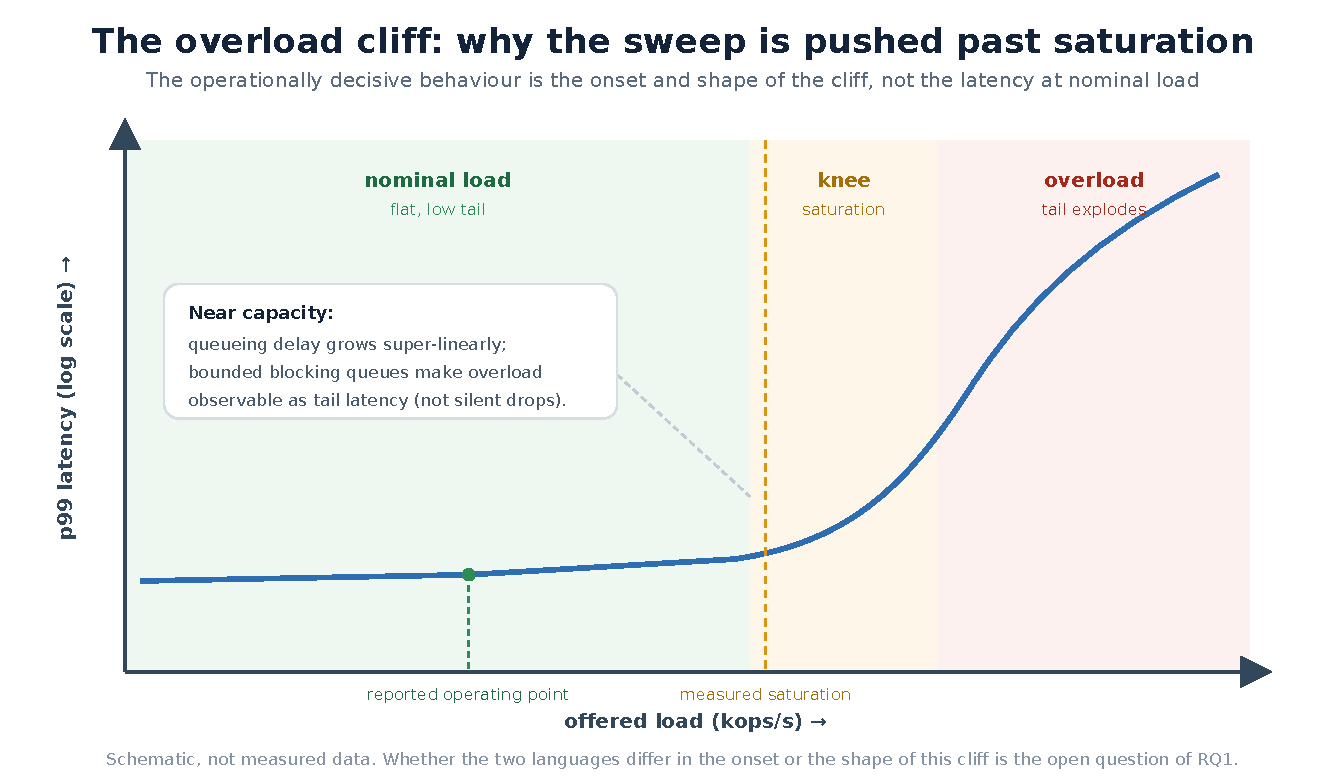
\includegraphics[width=0.70\linewidth]{diagrams/pdf/15_overload_cliff.pdf}
\caption[Vách quá tải]{Vách quá tải. Độ trễ đuôi thấp và phẳng khi tải đưa vào dưới công suất phục vụ, rồi
leo dốc mạnh khi hệ thống bị đẩy qua bão hoà và yêu cầu xếp hàng sau các hàng đợi chặn có giới
hạn. Hành vi quyết định vận hành là chỗ và hình dạng vách này bắt đầu, đó là lý do quét tải được
đẩy qua điểm bão hoà thay vì dừng ở tải danh định. Hình là sơ đồ hiện tượng chứ không phải đồ
thị dữ liệu nghiên cứu: liệu hai ngôn ngữ có khác ở chỗ vách bắt đầu hay độ dốc leo chính là điều
RQ1 hỏi, và Mục~\ref{sec:perfresults} báo cáo máy phát triển không phân giải được.\label{fig:cliff}}
\end{figure}

\chapter{Phương pháp nghiên cứu\label{chapter:methodology}}

Chương trước nêu nghiên cứu phải đạt gì. Chương này nêu cách đạt. Nó trình bày chiến lược
nghiên cứu tổng thể, phương pháp chọn cho từng câu hỏi nghiên cứu và vì sao phù hợp, các kiểm
soát giúp so sánh ngôn ngữ công bằng, xử lý thống kê các phép đo, cùng các cam kết tái lập và đạo
đức mà công trình tuân theo.

\section{Hướng tiếp cận nghiên cứu}\label{sec:approach}
Nghiên cứu mang tính thực nghiệm với yếu tố kiến tạo (khoa học thiết kế). Hiện vật là một cặp
bản hiện thực tương đương chức năng của phân hệ, một bằng C++ và một bằng Rust, cùng khung đo
hiệu năng. Cả hai được xây từ một đặc tả cố định duy nhất rồi đánh giá dưới thí nghiệm có kiểm
soát. Bằng chứng được tam giác hoá qua ba phương pháp. Đo hiệu năng dưới quét tải trả lời RQ1 và
RQ3, nghiên cứu tiêm lỗi có kiểm soát trả lời RQ2, và nghiên cứu tình huống di trú FFI, một
phần đo một phần định tính, trả lời RQ4. Ba phương pháp độc lập. Một điểm yếu ở một trong số
chúng, ví dụ độ nhạy môi trường của đo độ trễ đuôi, do đó không lan sang toàn bộ kết luận. Mỗi
phép đo báo cáo phương sai qua nhiều lần chạy lặp, và Mục~\ref{sec:controls} nêu các kiểm soát
giữ ngôn ngữ là biến duy nhất.

Thiết kế đó bám theo hình dạng các câu hỏi. Mỗi câu hỏi hỏi một kết quả (độ trễ đuôi, lỗi được
ngăn, dùng tài nguyên, chi phí di trú) phụ thuộc vào một biến, ngôn ngữ hiện thực. Ngôn ngữ vì
thế phải là khác biệt có hệ thống duy nhất giữa hai đối tượng thử. Điều này loại trừ dạng so
sánh ngôn ngữ phổ biến nhất trong tài liệu, nơi hai chương trình viết độc lập được đo và khoảng
cách quy cho ngôn ngữ. Khoảng cách đó còn mang thiết kế, thư viện và kỹ năng tác giả.

Xây cả hai phía từ một đặc tả loại bỏ nhiễu loạn đó. So sánh khi đó là giữa hai mã hoá của cùng
thiết kế, và hiện vật vừa là đóng góp vừa là dụng cụ đo nó. Ở nơi câu hỏi trả lời được bằng số,
xử lý là định lượng. Ở nơi không thể, như loại bảo đảm trong RQ2 và nỗ lực thiết kế API trong
RQ4, xử lý là định tính nhưng vẫn có hệ thống.

Khoảng trống mà thiết kế này nhắm tới (Mục~\ref{sec:gap}) chỉ tốt bằng tìm kiếm đã tìm nó, nên
tìm kiếm đó được lưu hồ sơ. Phụ lục~\ref{appendix:search} nêu cơ sở dữ liệu, tổ hợp thuật ngữ,
chuỗi trích dẫn và quy tắc lọc. Hai phát hiện của nó liên quan thiết kế chứ không chỉ thư mục tài
liệu.

Các luận văn do nhà cung cấp gần nhất nghiên cứu này (Mục~\ref{sec:relatedwork}) không có trong
cơ sở dữ liệu trích dẫn. Chuỗi trích dẫn do đó không chạm tới chúng, và chúng phải được tìm bằng
cách tra trực tiếp kho lưu trữ của cơ sở. Cùng các tìm kiếm đó cũng chứng minh sự vắng mặt phía
kia: không có luận văn Phần Lan về Rust trong bối cảnh truy nhập vô tuyến hoặc viễn thông, và
không có ấn phẩm được lập chỉ mục nhắc Rust từ nhà cung cấp chủ trì công trình. Tài liệu chuyên
ngành về câu hỏi ngôn ngữ do đó là tiếng Thụy Điển và do Ericsson lưu trữ, và liệu có chuyển
sang đây vẫn chưa được thử. Các luận văn đó là văn bản xám, nên được trích như bằng chứng về
điều một nhà cung cấp đã thử và thấy, không như kết quả đã bình duyệt.

Tìm kiếm không trả về nghiên cứu nào, có lập chỉ mục hay xám, đo hành vi độ trễ đuôi của hai bản
hiện thực Rust và C++ cùng một phân hệ mặt điều khiển có trạng thái, đồng thời, dưới quá tải.

Bảng~\ref{tab:design} ánh xạ mỗi câu hỏi nghiên cứu tới phương pháp, hiện vật, dữ liệu và chỉ số
trả lời nó. Cả bốn chuỗi cùng kết thúc ở một chỗ: Mục~\ref{sec:rqdiscussion} phán đoán từng câu
hỏi và Mục~\ref{sec:hypotheses} xử lý giả thuyết của nó. RQ1 và RQ3 dùng chung H1, diễn đạt để
bao cả tương đương hiệu năng theo nghĩa độ trễ và tài nguyên. Cách diễn đạt đó hóa ra là điểm yếu
chính của giả thuyết. RQ2 không nhạy môi trường, và RQ4 cũng vậy trừ một trục: thời gian biên
dịch là phép đo thời gian như mọi phép đo khác, nên được đọc như tỉ số giữa hai chuỗi công cụ đo
luân phiên trên một máy. RQ1 và RQ3 phụ thuộc máy đo và được báo cáo theo những gì máy đó chịu
được (Mục~\ref{sec:testbed}).

\begin{table}[H]
\centering
\caption[Thiết kế nghiên cứu: cách trả lời từng câu hỏi]{Thiết kế nghiên cứu: cách trả lời từng câu hỏi nghiên cứu. Mỗi câu hỏi gắn với một
phương pháp cụ thể, một hiện vật công bố, dữ liệu nó tạo ra, và chỉ số mà kết luận dựa vào. RQ1
và RQ3 mang hai phương pháp thay vì một: quét đo vòng khứ hồi mà một triển khai sẽ trải, còn phân
rã thành phần đo phần mà ngôn ngữ chịu trách nhiệm. Mục~\ref{sec:methodperf} nêu vì sao một cái
không thay được cái kia. RQ1 và RQ3 được kiểm với H1, RQ2 với H2, và RQ4 với H3.\label{tab:design}}
\renewcommand{\arraystretch}{1.25}
\begin{tabular}{@{}p{0.06\linewidth} p{0.24\linewidth} p{0.24\linewidth} p{0.32\linewidth}@{}}
\hline\hline
RQ & Phương pháp & Hiện vật / dữ liệu & Chỉ số chính \\
\hline
RQ1 & Quét tải tới quá tải, lặp xen kẽ & Khung đo, histogram độ trễ &
trung vị, độ trễ đuôi p99/p99.9, và cực đại so với tải đưa vào \\
RQ3 & Cùng quét, thu tài nguyên & Mẫu \texttt{getrusage} mỗi lần chạy &
RSS đỉnh, mức dùng CPU, thông lượng \\
RQ1, RQ3 & Phân rã thành phần: gọi lõi trực tiếp, rồi qua dịch vụ &
Cặp microbenchmark khớp, lặp xen kẽ &
chi phí mỗi thao tác tách thao tác và bàn giao giữa luồng \\
RQ2 & Tiêm lỗi có kiểm soát & Danh mục lỗi, ASan/TSan/UBSan, \texttt{rustc},
nhật ký Loom/Shuttle và Miri &
phân loại lớp lỗi (biên dịch / lúc chạy / không phát hiện) \\
RQ4 & Nguyên mẫu di trú FFI & Máy chủ C++ $+$ đường nối C-ABI Rust &
kích thước đường nối, phạm vi \texttt{unsafe}, chi phí tương tác mỗi lần gọi \\
\hline
\end{tabular}
\end{table}

\section{Phương pháp cho bốn câu hỏi nghiên cứu}
Bảng~\ref{tab:design} ghép mỗi câu hỏi với một phương pháp.

\subsection{Đo hiệu năng dưới quét tải (RQ1, RQ3)}\label{sec:methodperf}
RQ1 và RQ3 được trả lời bằng cách lái cả hai bản hiện thực với cùng một khối lượng công việc
tổng hợp xác định qua một quét tải đưa vào, từ tải nhẹ qua bão hoà tới quá tải. Hai quyết định
thiết kế làm phép đo đáng tin. Bộ sinh tải theo lịch \emph{vòng hở}: mỗi yêu cầu có thời điểm gửi
dự định cố định, và độ trễ được đo so với thời điểm đó chứ không so với lúc nhận. Điều đó sửa
coordinated omission như Chương~\ref{chapter:background} định nghĩa. Quét được đẩy qua bão hoà
cố ý, vì vách quá tải chỉ xuất hiện khi tải đưa vào vượt công suất phục vụ (Mục~\ref{sec:predictability}).
Độ trễ đi vào histogram dải động cao cấu hình giống hệt hai phía, và dùng tài nguyên (RSS cư
trú đỉnh, mức dùng CPU, thông lượng) được lấy mẫu qua hệ điều hành.

\paragraph{Đo cả thành phần lẫn vòng khứ hồi.}
Một vòng khứ hồi gói hai loại chi phí khác nhau. Một là thao tác ngôn ngữ chạy trong một luồng:
tra băm, bảo vệ máy trạng thái, cập nhật trường, tất cả do trình biên dịch sinh. Kia là bàn
giao quanh nó giữa các luồng: xếp hàng, đánh thức futex, chuyển ngữ cảnh, hoàn tất, không thuộc
ngôn ngữ. Chỉ phần đầu có thể khác giữa C++ và Rust, và không phép đo end-to-end nào tách chúng.

Phương pháp vì thế làm việc ở hai mức. Bộ xử lý thao tác được gọi trực tiếp, không có hàng đợi
trên đường đi, rồi qua dịch vụ đa luồng đầy đủ. Hiệu hai mức là bàn giao. Cả hai mức là trung
bình theo lô trên vòng lặp dài chứ không phải trung vị mỗi lần gọi, vì đọc đồng hồ tốn hàng chục
nano giây, cùng bậc với bản thân thao tác, và dấu thời gian mỗi lần gọi sẽ đo dụng cụ. Hai ngôn
ngữ xen kẽ qua các lần lặp và so sánh bằng cùng kiểm định ghép cặp chính xác như quét, nên hai
mức khác nhau ở điều đo chứ không ở cách phân tích.

Báo cáo cả hai tách hai câu hỏi mà các câu hỏi nghiên cứu ban đầu không phân biệt rõ: triển khai
hình dạng này sẽ trải gì, và ngôn ngữ đang làm gì. Mục~\ref{sec:budget} thấy hai mức cách nhau
hơn hai bậc độ lớn. Sự phân biệt do đó quyết định liệu kết quả có diễn giải được không. Mức thứ
hai được thêm sau vòng đầu chiến dịch, và Mục~\ref{sec:threats} ghi nhận sửa đổi đó.

\paragraph{Cô lập các nguyên thủ đồng bộ tranh chấp.}
So sánh quá tải ở Mục~\ref{sec:overload} quy khoảng cách cho hai mục forced-idiom nơi thư viện
chuẩn lệch nhau. Chúng là hàng đợi chặn có giới hạn và tay cầm hoàn tất một lần. Quy kết đó được
lập luận từ hình dạng phép đo dịch vụ đầy đủ, nên một microbenchmark khớp thứ ba lái hai nguyên
thủ đó một mình, không có công việc \texttt{ShardCore} trên đường đi, dưới cùng lặp xen kẽ và
kiểm định ghép cặp. Mục~\ref{sec:contention} nêu cấu hình và báo cáo liệu nguyên thủ cô lập có
tái tạo thứ tự mà dịch vụ đầy đủ cho thấy.

\subsection{Tiêm lỗi có kiểm soát (RQ2)}\label{sec:methodfaults}
RQ2 hỏi ngôn ngữ ngăn lớp lỗi nào. Đo mã không lỗi không trả lời được: vắng mặt lỗi trong kiểm
thử đậu không nói gì về việc ngôn ngữ có bắt được lỗi hay không. Phương pháp vì thế đối kháng,
theo thực hành đã thành lập của tiêm lỗi phần mềm, nơi lỗi được đưa vào cố ý để xem hệ thống
hành xử thế nào khi có lỗi~\cite{natella2016fault}.

Một danh mục các lỗi C++ đại diện được viết \emph{cố ý}, rút từ các lớp ảnh hưởng phân hệ này
(Chương~\ref{chapter:context}). Mỗi mục là chương trình nhỏ tự chứa mang hương miền: con trỏ cũ
vào bản đồ ngữ cảnh, giải phóng kép, thay đổi khi lặp, cập nhật dùng chung không đồng bộ. Mỗi mục
được biên dịch và chạy dưới AddressSanitizer, ThreadSanitizer và UndefinedBehaviorSanitizer, ghi
công cụ nào phát hiện, nếu có, và ở giai đoạn nào.

Cùng cấu trúc rồi được viết bằng Rust an toàn và biên dịch. Kết quả trình biên dịch được ghi, và
nếu biên dịch được thì hành vi chương trình cũng vậy. Các lớp ranh giới không cho trình biên dịch
gì để nói, nên phía Rust còn đi tới hai model checker, Loom và Shuttle, và với lớp nằm trong khối
\texttt{unsafe} tới trình thông dịch Miri. Chúng trả lời nửa ``ở giai đoạn nào và với chi phí gì''
của RQ2 cho các lớp đó, và mỗi cái được ghép với đối chứng trong đó lỗi đã sửa, để tìm lỗi và
báo cáo mọi thứ không trở thành cùng một quan sát.

Việc ThreadSanitizer báo đảo thứ tự khoá phụ thuộc lịch trình, nên một lần chạy sẽ ghi đúng kết
quả máy tình cờ cho. Runner chạy ca đó mười hai lần và báo tỉ lệ, để phát hiện gián đoạn không bị
nhầm là phát hiện đáng tin.

\paragraph{Vì sao phía C++ chỉ dùng sanitiser.}
Không có trình phân tích tĩnh nào chạy trên danh mục C++, và đó là quyết định. RQ2 không hỏi công
cụ nào tìm nhiều lỗi nhất. Nó hỏi ở \emph{giai đoạn} nào, và với lực gì, mỗi ngôn ngữ loại trừ
lỗi, và ba kết quả của phân loại (từ chối lúc biên dịch, phát hiện lúc chạy, bỏ sót im lặng) là
các hạng mục câu hỏi cần. Một lượt tùy chọn không thuộc hạng nào: cảnh báo mà bản dựng có thể cấu
hình bỏ qua là đối tượng khác với biên dịch không thể thành công, và khác biệt đó là điều phương
pháp đo.

Chi phí là phía C++ hẹp hơn điều tốt nhất một dự án C++ có thể làm, vì trình phân tích cấu hình
tốt có thể chạm các ca an toàn bộ nhớ nội thủ tục nhỏ, dù không chạm các ca đồng thời. Nghiên cứu
vì thế báo cáo công cụ đã chạy, thực hành dựa sanitiser ở Mục~\ref{sec:cpplatency}, chứ không phải
trần của công cụ C++.

Lỗi tiêm được giữ cố định trong khi ngôn ngữ thay đổi, nên mọi khác biệt kết quả đến từ bảo đảm
ngôn ngữ chứ không từ lỗi cụ thể. Phương pháp thiết lập \emph{loại} bảo vệ mỗi ngôn ngữ cung cấp,
không phải một con số hiệu năng.

Một quyết định thiết kế quyết định liệu phân loại đáng tin. Danh mục chỉ rút từ các lớp ngôn ngữ
đã biết là ngăn được có thể xác nhận giả thuyết nhưng không bao giờ làm lung lay nó, và sẽ mô tả
lựa chọn ca của tác giả nhiều như mô tả ngôn ngữ. Danh mục vì thế xây hai nhóm: các lớp trong
bảo đảm đã nêu của Rust, và các lớp ngay ngoài nó, nơi sở hữu và kỷ luật \texttt{Send}/\texttt{Sync}
không bảo vệ. Mỗi ca mang kỳ vọng ghi nhận và runner báo vi phạm theo cả hai chiều, nên kết quả
bất ngờ nổi lên như sai lệch thay vì bị hấp thụ vào tường thuật. Điều này đổi lấy một ranh giới
chứ không phải điểm số: nghiên cứu có thể nêu lớp nào ngôn ngữ loại bỏ và lớp tương đương nào còn
lại, đó là điều quyết định di trú cần.

\subsection{Nghiên cứu tình huống di trú giao diện hàm ngoại (RQ4)}\label{sec:methodffi}
RQ4 liên quan chi phí thực tế khi áp dụng Rust trong hệ C++ sẵn có, vừa là câu hỏi kỹ thuật vừa
là câu hỏi kỹ sư. Nó được trả lời bằng nguyên mẫu xây theo hướng di trú thực tế: máy chủ C++ gọi
thành phần Rust qua giao diện nhị phân ứng dụng C. Ba đại lượng được đo trên đó. \emph{Kích
thước} đường nối đếm điểm vào, dòng mã và phụ thuộc. \emph{Phạm vi} \texttt{unsafe} ghi nơi rời
ngôn ngữ được kiểm tra và liệu lõi an toàn có bị ảnh hưởng. \emph{Chi phí mỗi lần gọi} là giá
vượt ranh giới, đo so với cùng thao tác gọi bản địa để so sánh cô lập phần đường nối thêm vào.
Hai đại lượng đầu đọc từ mã, đại lượng thứ ba là cặp microbenchmark khớp. Ghép chúng tách chi phí
thời gian chạy của tương tác khỏi chi phí thật, nằm ở thiết kế API và học hỏi của con người.

Tương tác là một trong ba thuật ngữ RQ4 nêu, và nguyên mẫu chỉ trả lời nó một mình. Ba đại lượng
nữa bao hai thuật ngữ còn lại, chọn vì kỹ sư biên dịch chạm tới chúng trước mọi thứ đường nối có
thể cho thấy. \emph{Thời gian biên dịch} được đo sạch và tăng dần, cho thư viện lõi một mình và
cho mọi mục tiêu mặc định, với cùng số job và lặp xen kẽ hai phía để tải một máy rơi đều lên hai
chuỗi công cụ. \emph{Dấu chân tĩnh} được đo trên runner conformance, tệp thực thi duy nhất cả
hai ngôn ngữ dựng từ cùng đặc tả, và ở cả hai chính sách liên kết thay vì mặc định mỗi chuỗi công
cụ, vì hai mặc định khác nhau ở việc có liên kết thư viện chuẩn hay không và một cặp số đơn sẽ báo
lựa chọn đó như khác biệt ngôn ngữ. \emph{Bề mặt bên thứ ba} đếm crate bắc cầu mỗi cấu hình giải
quyết và các điểm \texttt{unsafe} bên trong, làm cho tuyên bố không phụ thuộc ở Mục~\ref{sec:idioms}
có thể kiểm. Đại lượng đầu nhạy máy chủ, hai kia thì không.

\section{Công bằng như chiến lược biến kiểm soát}\label{sec:controls}
Mỗi câu hỏi nghiên cứu quy một khác biệt cho ngôn ngữ, nên tính hợp lệ phụ thuộc giữ mọi thứ khác
bằng nhau. Công bằng vì thế là kiểm soát trung tâm của nghiên cứu, thực thi ở nhiều mức.

\emph{Đặc tả} được cố định trước khi viết mã. Nó khóa API công khai, máy trạng thái, cấu trúc
dữ liệu và chiến lược thuật toán của chúng, cùng mô hình sharding và đồng thời (Mục~\ref{sec:fairness}).
\emph{Nền thời gian chạy} được cân bằng bằng cách liên kết cùng bộ cấp phát hai phía và khớp mức
tối ưu hoá bản dựng gần nhất mà hai chuỗi công cụ cho phép. \emph{Khối lượng công việc} đến từ
một driver cấu trúc giống nhau giữa các ngôn ngữ, với một seed và quần UE hoạt động cho trước,
lái cả hai bản hiện thực qua cùng chuỗi thao tác. Mọi khác biệt độ trễ do đó phản ánh cách mỗi
ngôn ngữ thực thi cùng công việc, không phải khác công việc.

Ở nơi hai ngôn ngữ thật sự không diễn đạt được cùng cấu trúc, độ lệch được ghi trong nhật ký
forced-idiom. Điều còn không kiểm soát được, chủ yếu bất đối xứng kỹ năng một tác giả, được
thừa nhận là mối đe doạ tính hợp lệ (Chương~\ref{chapter:discussion}) và không được tuyên bố là
đã loại bỏ.

Bảng~\ref{tab:controls} nêu chiến lược theo từng biến, và cột thứ ba quan trọng nhất. Thí
nghiệm có kiểm soát đáng tin theo mức nó kế toán trung thực những gì không kiểm soát được. Ba
hàng ghi phần dư chứ không phải sửa sạch: ngôn ngữ không luôn diễn đạt được cùng cấu trúc, chúng
không ship cùng bố cục băm, và một người viết cả hai bản hiện thực. Nhật ký forced-idiom xử lý
điều đầu, và hàng cuối đặt tên biến duy nhất không còn kiểm soát nào.

\begin{table}[H]
\centering
\small
\caption[Chiến lược biến kiểm soát]{Chiến lược biến kiểm soát: điều được giữ cố định để ngôn ngữ vẫn là khác biệt có hệ thống
duy nhất, và điều mỗi kiểm soát không chạm tới. Cột thứ ba không phải danh sách sơ suất mà là
tự kể giới hạn của nghiên cứu. Mỗi mục được nối lại như mối đe doạ tính hợp lệ ở
Mục~\ref{sec:threats}. Chỉ hàng cuối đặt tên biến không có kiểm soát nào.\label{tab:controls}}
\footnotesize
\renewcommand{\arraystretch}{1.15}
\begin{tabular}{@{}R{0.16\linewidth} R{0.44\linewidth} R{0.32\linewidth}@{}}
\hline\hline
Biến & Cách giữ cố định & Điều kiểm soát không chạm tới \\
\hline
Thiết kế & Một đặc tả, cố định trước khi viết mã, khóa API công khai, máy trạng thái, cấu trúc dữ liệu và chiến lược thuật toán, cùng cách chia trạng thái thành shard (\S\ref{sec:fairness}) & Ở nơi hai ngôn ngữ không diễn đạt được cùng cấu trúc, độ lệch được ghi chứ không gỡ (Bảng~\ref{tab:idioms}) \\
Mô hình đồng thời & Một luồng mỗi shard qua hàng đợi MPSC chặn có giới hạn hai phía, không runtime bất đồng bộ ở phía nào & Không còn điểm mở \\
Băm & SplitMix64 cho chọn shard và FNV-1a trong shard, ghim giống nhau, để hasher mặc định của thư viện chuẩn không thành lợi thế tình cờ & Container vẫn là bản đồ băm riêng mỗi ngôn ngữ, và hai bên khác bố cục (\S\ref{sec:budget}) \\
Bộ cấp phát & Cùng \texttt{jemalloc} liên kết hai phía, với bản dựng bộ cấp phát hệ thống giữ làm đối chứng mỗi phía & Không còn điểm mở \\
Tối ưu hoá & \texttt{-O2} đối \texttt{opt-level~=~2} & Tương đương danh nghĩa không phải sinh mã giống hệt \\
Khối lượng công việc & Một driver xác định. Với seed và quần UE hoạt động cho trước cả hai bản hiện thực thực thi cùng chuỗi thao tác, kiểm bằng đếm theo loại & Tổng hợp và biện minh bằng đặc tả chứ không phát lại từ lưu lượng sản xuất \\
Dụng cụ đo & Cùng thuật toán và cấu hình histogram HDR, cùng lịch vòng hở, cùng kỷ luật lặp và xen kẽ & Không còn điểm mở \\
Hành vi & Bộ kiểm thử conformance trung tính ngôn ngữ với bản ghi chuẩn được diff từng thao tác (\S\ref{sec:parity}) & Tương đương giới hạn hành vi, không phải hiệu năng \\
\hline
Tác giả & Không kiểm soát & Một người viết cả hai bản hiện thực và không thành thạo như nhau cả hai ngôn ngữ \\
\hline
\end{tabular}
\end{table}

\section{Xử lý thống kê các phép đo}\label{sec:stats}
Các phép đo hiệu năng không xác định, nên số một lần chạy được tránh xuyên suốt. Mỗi cấu hình
(ngôn ngữ $\times$ bộ cấp phát $\times$ mức tải) được đo qua nhiều lần lặp độc lập, và bốn biến
thể được \emph{xen kẽ} trong mỗi lần lặp để trôi chậm, nhiệt và hoạt động nền làm nhiễu đều nhau
thay vì lệch một phía. Kết quả được tóm bằng trung vị với khoảng tin cậy bootstrap $95\%$
không tham số~\cite{efron1993bootstrap} thay vì trung bình với độ lệch chuẩn, vì phân phối độ
trễ đuôi nặng và lệch và khoảng không tham số trên trung vị không giả định chuẩn. Cách này bám
hướng dẫn đã thành lập về đánh giá hiệu năng có thống kê chặt, cảnh báo báo cáo một số duy mời
kết luận mà biến thiên giữa các lần chạy không ủng hộ~\cite{georges2007rigorous}. Các phân vị đuôi
(p99, p99.9, p99.99) đọc từ histogram HDR, có gom nhóm logarit giữ ba chữ số có nghĩa trên toàn
dải để các phân vị cao không bị lượng tử hoá mất. Khoảng được báo đầy đủ, không phải nửa độ rộng
đối xứng, vì khoảng bootstrap trên trung vị của mẫu đuôi nặng lệch rõ và nửa độ rộng đủ che biên
trên sẽ đặt biên dưới dưới không.

Hai đại lượng này cần ghi chú riêng, vì mức sâu vào đuôi mà một chiến dịch nhìn thấy là thuộc tính
của số thao tác đã ghi. Ở tải đại diện một lần chạy hoàn tất cỡ $170$~nghìn thao tác đo, nên
p99.99 của nó dựa trên khoảng mười bảy quan sát: p99.99 mỗi lần chạy bị nhiễu lấy mẫu chi phối
ngay cả trên máy hoàn toàn yên. Đọc đuôi xa vì thế đòi lưu toàn bộ nội dung bucket HDR mỗi lần
chạy cạnh các phân vị tóm tắt, để các lần lặp có thể được \emph{gộp} thành một phân phối vài
triệu thao tác trước. Khung làm vậy hiện nay, và thiết kế tách gộp và lấy trung bình, vì chúng
là hai thống kê khác nhau. Một số gộp sẽ lấy thao tác làm đơn vị phân tích và phân giải đuôi xa,
với chi phí không mang khoảng giữa các lần lặp, trong khi các số trung vị-của-lần-lặp báo cáo
kèm khoảng giữ lần lặp làm đơn vị và vẫn là cơ sở duy nhất cho so sánh ghép cặp. Jitter cũng sẽ
được đo trực tiếp thay vì suy từ phân phối độ trễ, như hiệu trị tuyệt đối giữa độ trễ liên tiếp
trong một producer. Đó là đại lượng biến thiên độ trễ gói của RFC~3393~\cite{rfc3393}, và khớp
cách luận văn dùng thuật ngữ: biến thiên từ thao tác này sang thao tác kế, không phải độ trải của
cả phân phối. Cả hai không được báo cáo ở Chương~\ref{chapter:eval}, vì chiến dịch phân tích ở đó
trước khi có dụng cụ đo (Mục~\ref{sec:perfresults}).

Dù vậy p99.99 hay jitter cũng không vào họ kiểm định ghép cặp mô tả dưới đây. Điều đó bám cùng
quy tắc với phần còn lại của thiết kế chứ không phải hệ quả của dữ liệu thiếu: cả hai tính từ
đúng các thao tác mà nhiễu giao thoa chạm tới, tức lớp thống kê mà ghép cặp không cứu được, nên
khoảng ghép cặp trên chúng không thể đọc như hiệu ứng ngôn ngữ. Chúng thuộc cột mô tả, và họ
kiểm định giữ cỡ mà thiết kế cam kết.

Chỉ khoảng ước lượng thì là cơ sở yếu cho so sánh. Hai khoảng có thể chồng trong khi một biến thể
dẫn ở mọi lần lặp, và chúng có thể tách trên khác biệt không tái lập. Nghiên cứu vì thế cũng
kiểm định trực tiếp so sánh, và thiết kế xen kẽ là điều làm điều đó khả thi: vì bốn biến thể
được đo liền nhau trong mỗi lần lặp, các lần chạy tạo thiết kế khớp mà nhiễu chung của một khối
triệt tiêu trong hiệu ghép cặp. Ngôn ngữ được so với ngôn ngữ với bộ cấp phát giữ cố định, dùng
kiểm định hoán vị ghép cặp hai phía chính xác trên hiệu theo lần lặp. Giả thuyết không là mỗi cặp
chỉ khác nhiễu giữa các lần chạy, dưới đó dấu mỗi hiệu ghép cặp có thể hoán đổi. Với số lần lặp
dùng ở đây mọi một trong $2^{n}$ gán dấu được liệt kê thay vì lấy mẫu, nên $p$-value thu được là
chính xác và, như bootstrap, không giả định gì về hình dạng phân phối. Vì cùng so sánh được làm
cho nhiều chỉ số và cả hai bộ cấp phát, họ kiểm định được hiệu chỉnh bằng thủ tục Holm bước
xuống~\cite{holm1979simple}, kiểm soát tỉ lệ lỗi họ mà không giả định độc lập giữa các kiểm định.

Hai quyết định về cách đọc họ đó được đưa ra ở đây chứ không sau kết quả, vì một trong hai có thể
bị chọn cho hợp dữ liệu nếu không.

Quyết định thứ nhất là so sánh nào vào họ, và câu trả lời phụ thuộc điểm vận hành chứ không phụ
thuộc chỉ số. Dưới bão hoà mọi biến thể hoàn tất công việc nhanh bằng tốc độ được đưa vào, nên
thông lượng đạt được ở đó bị ghim vào tải đưa vào theo cấu trúc và không thể biểu đạt hiệu ứng
ngôn ngữ dù ngôn ngữ làm gì. Nó được báo cáo kèm khoảng thay vì được kiểm. Trên bão hoà lập luận
đảo ngược, vì điều mỗi biến thể vẫn duy trì không bị ghim vào gì và trở thành đại lượng duy nhất
có thể tách chúng, nên một điểm vận hành thứ hai được cố định trong vùng quá tải và thông lượng
duy trì cùng mức dùng CPU được kiểm ở đó (Mục~\ref{sec:overload}). Hai cam kết đi kèm. So sánh
quá tải gia nhập cùng họ Holm thay vì tạo họ thứ hai, để chia hai điểm vận hành không bị đọc như
tách chọn sau khi đã biết $p$-value. Và không phân vị độ trễ nào được kiểm trên bão hoà, vì
producer không theo kịp lịch dự định cố định sẽ tụt lại tích luỹ, khiến các phân vị ở đó là cận
dưới chứ không phải ước lượng. Phụ lục~\ref{appendix:stats} nêu lập luận sau cả hai.

Quyết định thứ hai là kết luận gì khi khoảng và $p$-value mâu thuẫn. Ở số lần lặp vừa phải chúng
thường sẽ: khoảng ghép cặp có thể nằm hoàn toàn một phía không trong khi $p$-value đã hiệu chỉnh
vẫn xa mọi ngưỡng thông dụng. Tin dụng cụ nào không phải lựa chọn tự do, và không phụ thuộc chỉ số
có hấp dẫn hay không. Nó phụ thuộc liệu ghép cặp có gỡ nhiễu mà phép đo đó chịu hay không. Ghép
cặp triệt tiêu mọi thứ một khối xen kẽ chia sẻ. Nó không triệt tiêu nhiễu rơi vào một lần chạy
của cặp mà không rơi vào lần kia. Tóm tắt mức lần chạy như RSS đỉnh không bị lay bởi vài thao tác
bị lên lịch lại, và thống kê bậc trung tâm như trung vị của hàng chục nghìn mẫu mỗi thao tác cũng
vậy. Với những đại lượng đó, hiệu ghép cặp giữ dấu qua các lần lặp là khác biệt trong phần mềm.
Phân vị cao là trường hợp ngược: p99 và p99.9 tính từ đúng các thao tác bị quấy, nên khoảng loại
trừ không có thể vừa khớp một lần chạy của cặp không may mắn vừa khớp hiệu ứng thật. Bảng~\ref{tab:significance}
vì thế được chia khối theo phân biệt đó, và khoảng ở khối thứ hai không được đọc như phát hiện dù
cách không bao nhiêu so với không. Áp quy tắc cho khối thuận lợi và lặng bỏ khối kia là đúng lỗi
mà cam kết trước này tồn tại để ngăn.

Độ phân giải mà thiết kế đạt được bị giới hạn bởi số lần lặp, và được nêu rõ chứ không để ngầm.
Với \NRepeats{} lần lặp và \NTests{} so sánh, sàn hai phía chính xác của kiểm định là
$\MinAttainableP$, và $\CorrectedFloor$ sau hiệu chỉnh, nên null báo ở đây phản ánh dữ liệu chứ
không phải số học. Trích cả hai là cách để độc giả phân biệt kết quả null và kết quả không phân
giải được. Chọn số lần lặp để sàn đã hiệu chỉnh nằm dưới $5\%$ thông dụng vì thế là phần giao thức
đo, cùng với ghim đồng hồ và cô lập lõi (Mục~\ref{sec:testbed}). Phụ lục~\ref{appendix:stats} suy
ra hai sàn.

\section{Tái lập và hiện vật nghiên cứu}\label{sec:repro}
Nghiên cứu được thiết kế để bên thứ ba tái tạo kết quả mà không cần mã độc quyền của Nokia. Ba
điều làm điều đó khả thi. Các bản hiện thực được lái hoàn toàn bởi đặc tả công khai đã cố định.
Khung đo, danh mục lỗi và runner của nó, cùng nguyên mẫu FFI được công bố cùng luận văn. Và mọi
hình và bảng trong phần đánh giá do một script duy nhất tạo trực tiếp từ nhật ký đo thô, nên
chạy lại chiến dịch trên máy khác tái tạo hiện vật nguyên văn.

Môi trường thực thi được ghi tự động cạnh mỗi tập kết quả: kiểu CPU, kernel, phiên bản trình
biên dịch và chuỗi công cụ, cùng cài đặt tần số và lập lịch của testbed. Điều kiện của một phép
đo vì thế đi cùng dữ liệu. Điều đó quan trọng cho một phân biệt cụ thể. Tách kết quả nhạy môi
trường (quét hiệu năng) khỏi kết quả không nhạy (kiểm thử tương đương, tiêm lỗi, và cấu trúc FFI)
là điều cho phép luận văn nêu, theo từng kết quả, độc giả đang nhìn loại nào. Không gì trên đường
đi đòi mã nguồn độc quyền, đó là điều làm tái lập bên thứ ba khả thi chứ không chỉ được phép.

\chapter{Thiết kế và Triển khai\label{chapter:design}}

\section{Đặc tả dùng chung: chuẩn công bằng}
\label{sec:fairness}
Trước khi viết bất kỳ mã nào, một đặc tả đã được đóng băng, và không phần nào trong đó gọi tên một ngôn ngữ.
Đặc tả cố định API công khai, máy trạng thái UE, cấu trúc dữ liệu và thuật toán đứng sau chúng
(bản đồ băm phân mảnh theo mã định danh UE, ví dụ), mức chi tiết của khóa và
phân mảnh, và mô hình đồng thời. Cả hai triển khai tuân theo đặc tả. Điều đó giữ cho
so sánh là so sánh hai ngôn ngữ, chứ không phải hai thiết kế hay hai mức kỹ năng. Đặc tả
là một sản phẩm độc lập, và là biện pháp kiểm soát chính chống
thiên lệch triển khai.

\section{Mô hình khái niệm và thiết kế đồng thời}\label{sec:concurrency}
Hai triển khai được xây dựng theo đặc tả dùng chung, và chúng làm cùng một việc: một
bản C++ hiện đại (C++23, STL, RAII, luồng chuẩn) và một bản Rust (bộ công cụ ổn định,
mô hình bộ nhớ dựa trên ownership, đồng thời an toàn). Cả hai dùng một mô hình đồng thời, mô tả là
\emph{không chia sẻ, một luồng cho mỗi shard}, cách mà RAN L3 thực tế chia trạng thái UE. Mô hình async và
mô hình dựa trên luồng không bao giờ được trộn, và đó là có chủ ý.

Không gian mã định danh UE được chia thành $N_{\text{shards}}$ shard, và mỗi shard thuộc về
đúng một luồng worker. Tám là mặc định. Chiến dịch đo ghim bảy thay vì, để
mỗi worker và mỗi producer sở hữu một trong các lõi được ghim, như
Mục~\ref{sec:testbed} ghi lại. Chỉ worker sở hữu đọc hoặc thay đổi ngữ cảnh của shard mình.
Worker do đó không chia sẻ trạng thái có thể thay đổi, và dữ liệu ngữ cảnh không cần khóa. Caller (các
luồng bộ tạo tải) không chạm trực tiếp vào trạng thái ngữ cảnh. Chúng gửi thông điệp yêu cầu vào
hàng đợi MPSC có giới hạn của một shard, rồi chờ trên tay cầm hoàn tất dùng một lần
mà worker ghi kết quả vào. Hàng đợi là \emph{có giới hạn và
chặn}. Khi hàng đợi của một shard đầy, gửi yêu cầu bị chặn cho đến khi có chỗ trống. Đó là điều
tạo ra độ trễ xếp hàng thực tế khi quá tải, và cũng là điều làm độ trễ đuôi
quan sát được, vì chính sách bỏ yêu cầu thay vì chặn sẽ che giấu
quá tải. Yêu cầu tới cùng một shard chạy nghiêm ngặt theo thứ tự vào trước ra trước.

Cấu trúc này cho so sánh đồng thời an toàn có thứ để đo. Cơ chế
được thử nghiệm là hàng đợi, bàn giao hoàn tất, và chuyển ownership của mỗi yêu cầu, chứ không phải
xung đột khóa. Một phần trạng thái có thể thay đổi được chia sẻ được phép: một bộ đếm nguyên tử ghi
số thứ tự hoạt động theo ngữ cảnh. Nó chỉ là ghi sổ, và không nhánh luồng điều khiển
phụ thuộc giá trị của nó. Độ trễ được đo trên toàn đường đi, từ thời điểm gửi dự kiến đến hoàn tất,
nên nó bao gồm độ trễ xếp hàng khi có tải và bao phủ cùng một vòng qua luồng trên cả hai
bên. Mục~\ref{sec:budget} sau đây tách số liệu thành phần ngôn ngữ thực thi và
phần hệ điều hành đảm nhiệm. Hình~\ref{fig:arch} cho thấy luồng dữ liệu, và
Hình~\ref{fig:reqlifecycle} truy vết một thao tác qua đó theo trình tự.

\begin{figure}[ht]
\centering
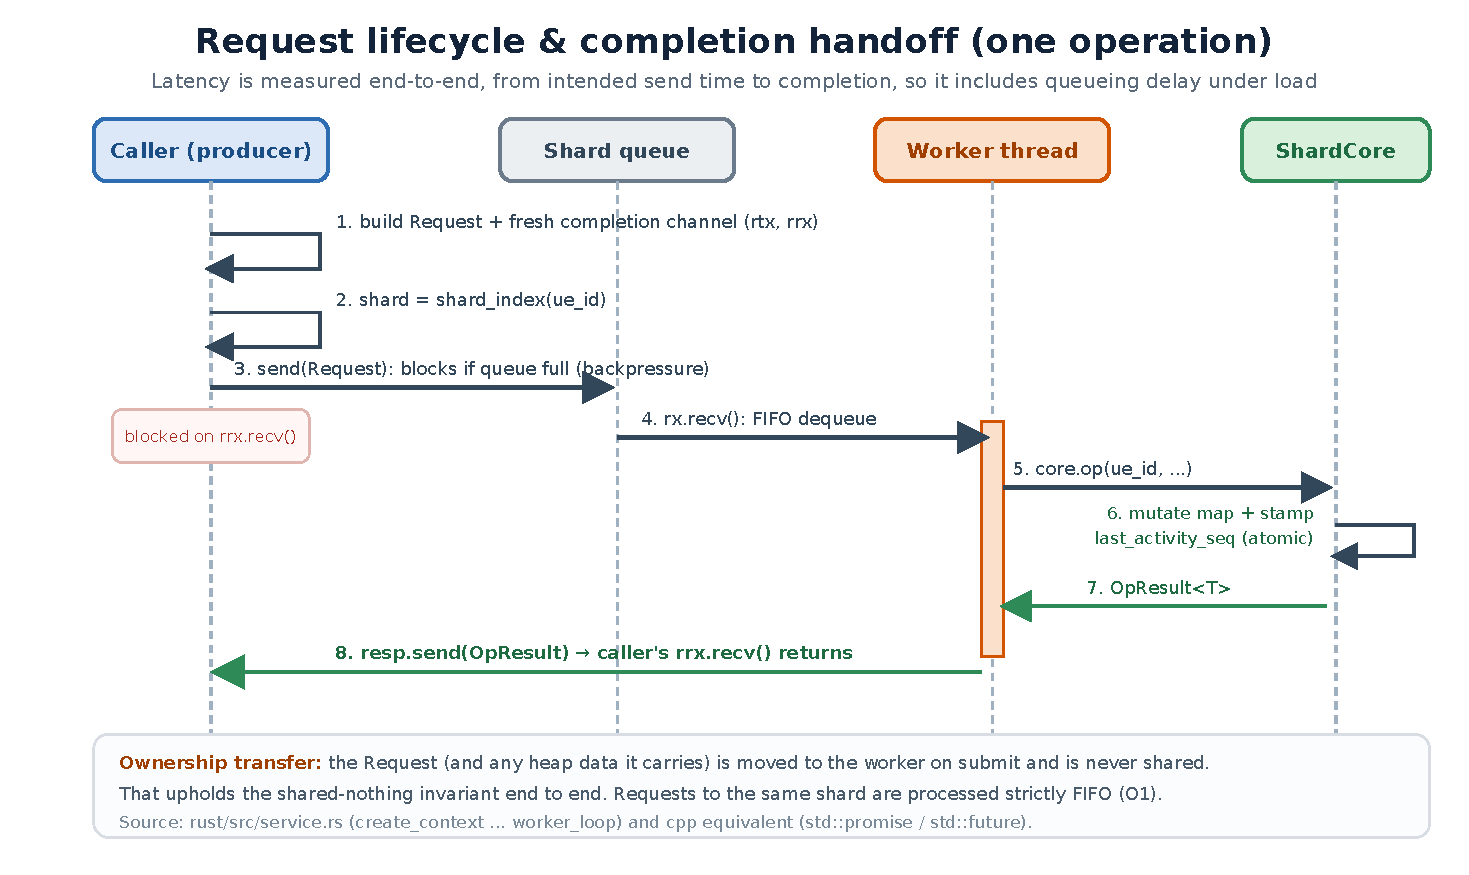
\includegraphics[width=0.78\linewidth]{diagrams/pdf/04_request_lifecycle_sequence.pdf}
\caption[Đường đi end-to-end của một thao tác]{Đường đi end-to-end của một thao tác và bàn giao hoàn tất. Caller xây dựng
một yêu cầu với tay cầm hoàn tất dùng một lần, định tuyến theo \texttt{shard\_index(ue\_id)} tới
hàng đợi có giới hạn của shard sở hữu (chặn nếu đầy), và chờ. Worker duy nhất của shard
dequeue theo thứ tự FIFO, thực thi thao tác trên store chỉ mình sở hữu, và ghi
kết quả trở lại tay cầm hoàn tất. Ownership của yêu cầu được chuyển cho worker khi
gửi và không bao giờ chia sẻ. Độ trễ được đo trên toàn đường đi.\label{fig:reqlifecycle}}
\end{figure}

\begin{figure}[ht]
\centering
\begin{tikzpicture}[
    font=\small,
    prod/.style={draw, rounded corners, minimum width=2.0cm, minimum height=0.66cm, fill=blue!8},
    queue/.style={draw, minimum width=2.5cm, minimum height=0.66cm, fill=gray!12},
    worker/.style={draw, rounded corners, minimum width=2.1cm, minimum height=0.66cm, fill=red!8},
    store/.style={draw, cylinder, shape border rotate=90, aspect=0.25, minimum width=1.5cm, minimum height=0.85cm, fill=green!8},
    lane/.style={draw, dotted, rounded corners, inner sep=7pt},
    >={Stealth[length=2.4mm]}
  ]
  % producers, grouped in one box to avoid a tangle of crossing arrows
  \node[prod] (p1) at (0,1.3)  {Producer 1};
  \node[prod] (p2) at (0,0.0)  {Producer 2};
  \node[prod] (p3) at (0,-1.3) {Producer $m$};
  \begin{scope}[on background layer]
    \node[draw, dashed, rounded corners, fill=blue!3, fit=(p1)(p2)(p3), inner sep=6pt] (pg) {};
  \end{scope}
  \node[font=\scriptsize] at (0,-2.15) {bộ tạo tải};

  % two representative shard lanes; spacing leaves room for the inline edge labels
  \node[queue] (q1) at (5.2,1.3)   {hàng đợi MPSC};
  \node[worker](w1) at (8.9,1.3)   {Worker 1};
  \node[store] (s1) at (12.0,1.3)  {Shard 1};
  \node[queue] (qn) at (5.2,-1.3)  {hàng đợi MPSC};
  \node[worker](wn) at (8.9,-1.3)  {Worker $N$};
  \node[store] (sn) at (12.0,-1.3) {Shard $N$};
  \begin{scope}[on background layer]
    \node[lane, fit=(q1)(s1)] (lane1) {};
    \node[lane, fit=(qn)(sn)] (lanen) {};
  \end{scope}
  \node[font=\scriptsize] at (8.35,2.35) {luồng sở hữu shard: không trạng thái chia sẻ, không khóa};

  % submit: producer group -> each shard queue, routed by hash
  \node[font=\scriptsize, align=center, fill=white, inner sep=2pt] at (2.85,0) {định tuyến theo\\ hash(\texttt{ue\_id})};
  \draw[->] (pg.east) -- (q1.west) node[midway, above, sloped, font=\scriptsize]{gửi};
  \draw[->] (pg.east) -- (qn.west) node[midway, below, sloped, font=\scriptsize]{gửi};

  % within-lane flow
  \draw[->]  (q1) -- node[above, font=\scriptsize]{FIFO} (w1);
  \draw[->]  (qn) -- node[above, font=\scriptsize]{FIFO} (wn);
  \draw[<->] (w1) -- node[above, font=\scriptsize]{sở hữu} (s1);
  \draw[<->] (wn) -- node[above, font=\scriptsize]{sở hữu} (sn);

  % one-shot completion: clean orthogonal return path below everything
  \draw[->, dashed, rounded corners=4pt]
      (wn.south) -- ++(0,-0.75) -- (1.4,-2.9) -- ($(pg.south east)+(-0.4,0)$);
  \node[font=\scriptsize] at (5.9,-3.05) {hoàn tất một lần (kết quả $\rightarrow$ producer đang chờ)};
\end{tikzpicture}
\caption[Kiến trúc không chia sẻ, một luồng cho mỗi shard]{Kiến trúc không chia sẻ, một luồng cho mỗi shard. Producer gửi thông điệp yêu cầu tới
hàng đợi MPSC có giới hạn, chặn của một shard (chọn bằng hash ghim của \texttt{ue\_id}) và chờ
trên tay cầm hoàn tất dùng một lần. Mỗi shard chỉ được đọc và ghi bởi đúng một luồng worker,
nên không có khóa trên trạng thái ngữ cảnh. Chặn khi hàng đợi đầy là điều làm quá tải
quan sát được như độ trễ đuôi.\label{fig:arch}}
\end{figure}

\section{Lựa chọn kiến trúc và ngăn xếp công nghệ}
Bên C++ dùng CMake với Ninja, thư viện chuẩn, và \texttt{std::thread}. Bên
Rust dùng Cargo và bộ công cụ ổn định. Cả hai liên kết cùng một bộ cấp phát bộ nhớ, điều đó giữ
so sánh về hai ngôn ngữ chứ không phải hai bộ cấp phát: C++ liên kết
\texttt{jemalloc} của hệ thống, và Rust cài một bộ cấp phát toàn cục \texttt{jemalloc} (từ
\texttt{tikv-jemallocator}). Mỗi bên cũng giữ một bản build với bộ cấp phát hệ thống làm đối chứng.
Độ trễ đi qua cùng thuật toán histogram HDR (HDR)~\cite{tene_hdrhistogram} trên cả hai bên, cấu hình giống nhau (phạm vi
$[1\,\text{ns}, 3.6\,\text{s}]$, ba chữ số có nghĩa). Rust dùng crate
\texttt{hdrhistogram} chuẩn. C++ dùng bản port header-only của cùng thuật toán gom nhóm,
được kiểm tra với phân phối đã biết. Tối ưu build được khớp gần nhất mà hai
bộ công cụ cho phép, nên profile release của Rust được ghim ở \texttt{opt-level~=~2} so với
build C++ \texttt{-O2}.

\section{Chi tiết triển khai}\label{sec:impldetails}
\label{sec:impl}
Cả hai triển khai tuân theo đặc tả đóng băng từng trường, và cả hai đủ nhỏ
để đọc từ đầu đến cuối. Lõi C++ là $\CppRawLines$ dòng trên tám header và hai
translation unit. Lõi Rust là $\RustRawLines$ dòng trên tám module. Bỏ dòng trống
và comment còn $\CppNloc$ và $\RustNloc$. Cả hai số mô tả build mà
chiến dịch thực sự đo. Một flag build bật hai thăm dò gán như Mục~\ref{sec:idioms}, và các khối điều kiện chọn chúng được bỏ khỏi số liệu,
vì đếm chúng sẽ mô tả không phải build được so sánh cũng không phải thăm dò.

Bản Rust do đó lớn hơn, $\RawRise\%$ theo dòng thô và
$\NlocRise\%$ theo dòng mã. Điều đó nên nằm trong văn bản chứ không phải chú thích cuối trang, vì hai lý do.
Số dòng là một trong các proxy chất lượng phần mềm mà nghiên cứu này đặt ra để thu thập. Và
khác biệt không phải dư thừa ngẫu nhiên: nó là kết quả ròng của nhiều điểm bắt buộc kéo theo chiều
ngược nhau, mà Mục~\ref{sec:idioms} phân tích từng file. Phần còn lại của mục này
đi từ mô hình dữ liệu ra cơ chế đồng thời, và báo cáo chi phí mỗi
phân kỳ buộc theo ngôn ngữ khi nó xuất hiện.

\subsection{Ngữ cảnh UE và máy trạng thái}\label{sec:uecontext}
Mỗi ngữ cảnh UE lưu mã định danh, trạng thái vòng đời (enumeration bốn giá trị
\texttt{Idle}, \texttt{Connected}, \texttt{Reconfiguring}, \texttt{Released}), cell phục vụ,
mã giao dịch RRC, một ngữ cảnh bảo mật giả 32 byte, danh sách động tối đa tám data
radio bearer, và hai bộ đếm (số thông điệp xử lý và số thứ tự hoạt động). Danh sách data
radio bearer cố ý là container có thể mở rộng (\texttt{std::vector} / \texttt{Vec})
chứ không phải mảng cố định, để nghiên cứu bộ cấp phát (RQ3) quan sát cấp phát
thực tế theo ngữ cảnh. Đọc trả về bản sao bất biến (\texttt{UeContextView}) sao chép ra từ
worker, không phải tham chiếu vào trạng thái shard đang sống. Điều đó giữ cam kết không chia sẻ
và giữ hai triển khai giống nghĩa hoàn toàn.
Hình~\ref{fig:datamodel} cho thấy bản ghi và đường đọc đầy đủ.

Khai báo trường giống hệt không tạo ra object giống hệt. Đo trên
máy đánh giá, \texttt{UeContext} chiếm $\CppUeCtxBytes$~byte trong C++ và chỉ
$\RustUeCtxBytes$~byte trong Rust.
Chính sách bố cục giải thích toàn bộ. C++ đảm bảo member dữ liệu không tĩnh nằm
theo thứ tự khai báo, nên enumeration một byte \texttt{state} giữa
mã định danh tám byte và cell id bốn byte buộc $\CppUeCtxStatePad$~byte padding, và
khóa bảo mật 32 byte, kết thúc ở offset $\CppUeCtxKeyEnd$, buộc thêm $\CppUeCtxKeyPad$ trước vector bearer căn tám byte. Rust không có chú thích \texttt{\#[repr(C)]} ở đây, nên có thể sắp xếp lại
trường, và nó làm vậy. Nó gom các scalar nhỏ và cả hai lỗ hổng biến mất.

Đặc tả không cố xóa khác biệt đó, và lý do cần nói rõ.
Ghim bố cục Rust bằng \texttt{\#[repr(C)]} sẽ phạt Rust chỉ vì tuân thủ
quy tắc padding của C++. Sắp xếp lại khai báo C++ thủ công sẽ là tối ưu mà
đặc tả không yêu cầu bên nào. Khoảng cách do đó được ghi là hiệu ứng cấp ngôn ngữ và
sau đó được giới hạn. Với $\SweepUes$ UE hoạt động mà sweep dùng, khoảng $\UeCtxGapBytes$ byte
tương đương khoảng $\UeCtxGapTotalKB$~kB. RSS được đo bằng megabyte, nên điều này
không ảnh hưởng so sánh RQ3.

\begin{figure}[ht]
\centering
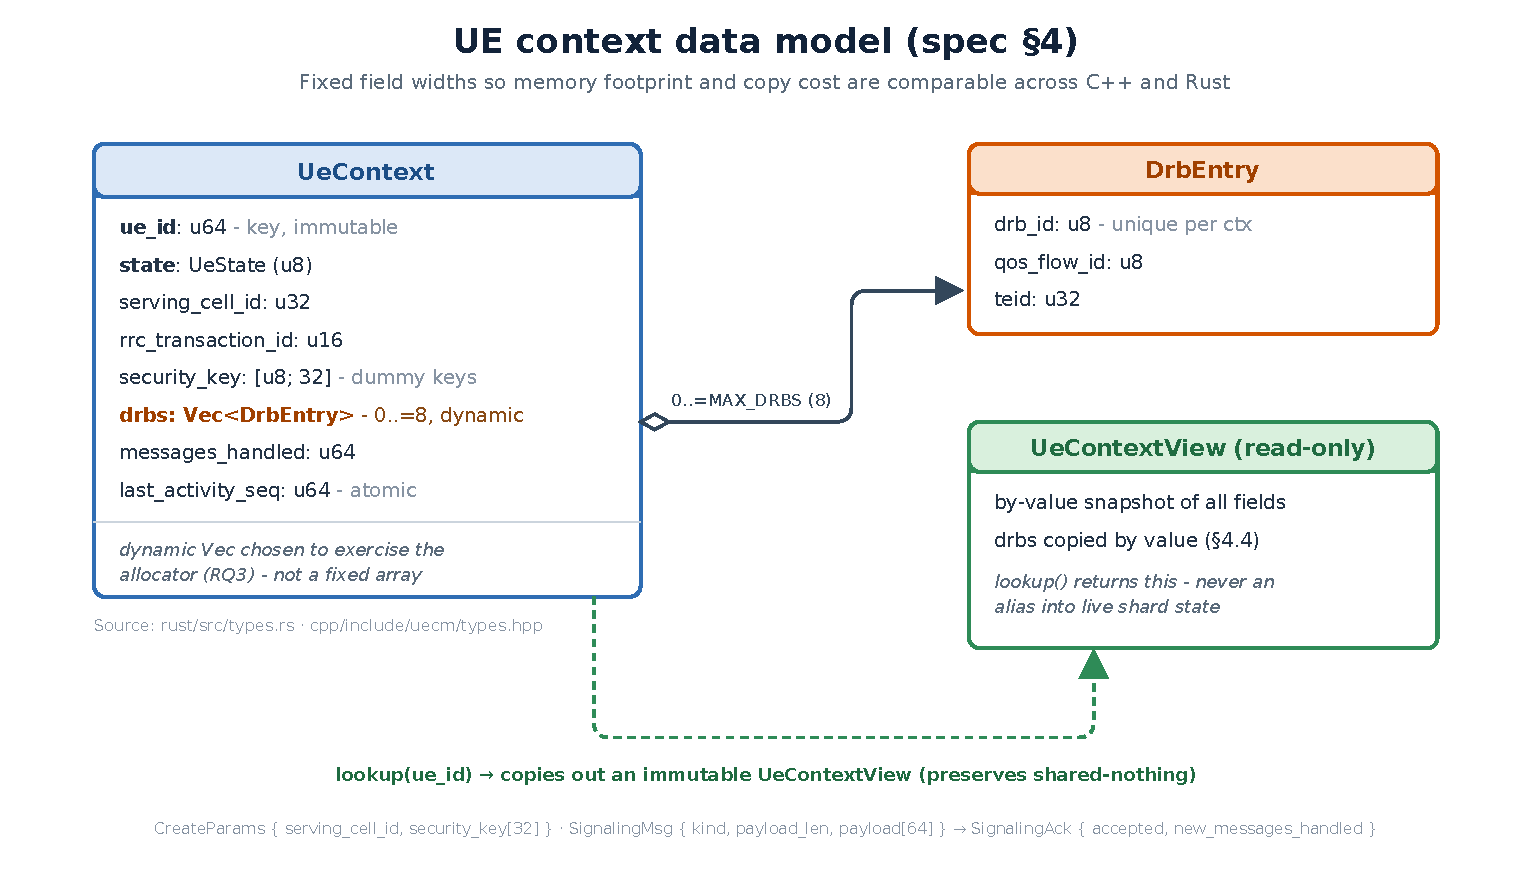
\includegraphics[width=0.72\linewidth]{diagrams/pdf/05_data_model.pdf}
\caption[Mô hình dữ liệu ngữ cảnh UE dùng chung]{Mô hình dữ liệu ngữ cảnh UE dùng chung cho cả hai triển khai. Chiều rộng trường được cố định để
dấu chân bộ nhớ và chi phí sao chép có thể so sánh giữa ngôn ngữ. Danh sách data-radio-bearer là
\texttt{Vec}/\texttt{std::vector} động có chủ ý, để kích hoạt bộ cấp phát cho RQ3.
\texttt{lookup} trả về \texttt{UeContextView} bất biến sao chép theo giá trị chứ không phải
alias vào trạng thái shard đang sống, giữ cam kết không chia sẻ.\label{fig:datamodel}}
\end{figure}

Bản ghi được điều khiển bởi vòng đời của Hình~\ref{fig:fsm}. Mỗi thao tác là một
chuyển trạng thái có bảo vệ, và Bảng~\ref{tab:transitions} cho bảng triển khai đầy đủ.
Hai tính chất giữ ở mọi nơi, và chúng là điều làm hai triển khai có thể so sánh từng
thao tác. Thứ nhất, mỗi thao tác kiểm tra trước khi thay đổi bất cứ gì. Chuỗi bảo vệ xác thực
mã định danh, tìm ngữ cảnh, kiểm tra trạng thái, và trả \texttt{OpError} khớp
trước khi chạm trường nào. Thao tác bị từ chối do đó để ngữ cảnh
bit-identical với trước đó. Thứ hai, không thao tác nào có thể thành công một phần, vì mỗi thao tác chỉ
thực hiện tối đa một đột biến sau bảo vệ cuối.

Hai hành vi cần nói rõ, vì bảng che chúng. Trạng thái
\texttt{Released} thực sự không được lưu. \texttt{release\_context} xóa entry
khỏi map shard hoàn toàn, nên \texttt{Released} chỉ là nhãn đi qua trong
đặc tả chứ không phải giá trị triển khai có thể bị bắt khi nghỉ. Lần
release thứ hai do đó trả \texttt{NotFound} chứ không phải \texttt{InvalidState}.
Trường hợp khác là \texttt{abort\_reconfigure}. Nó khôi phục \emph{trạng thái} về
\texttt{Connected}, nhưng không khôi phục serving cell mà \texttt{begin\_reconfigure}
đã ghi đè bằng mục tiêu handover. Đó là đơn giản hóa có chủ ý, vì mô hình không
lưu cell trước handover để rollback. Vẫn là cam kết ngữ nghĩa chứ không phải sơ suất,
và cả hai triển khai làm giống nhau, điều bộ parity của
Mục~\ref{sec:parity} kiểm tra.

\begin{table}[H]
\centering
\small
\caption[Bảng chuyển trạng thái triển khai]{Bảng chuyển trạng thái triển khai, giống hệt ở cả hai ngôn ngữ. Mọi thao tác
còn trả \texttt{InvalidArgument} cho \texttt{ue\_id} bằng không, và thao tác bị từ chối
để ngữ cảnh không thay đổi. \texttt{Released} không bao giờ được lưu: release xóa
entry.\label{tab:transitions}}
\begin{tabular}{@{}l l l R{0.31\linewidth}@{}}
\hline\hline
Thao tác & Trạng thái yêu cầu & Trạng thái kết quả & Lỗi \\
\hline
\texttt{create\_context}       & ngữ cảnh không có   & \texttt{Idle}          & \texttt{AlreadyExists}, \texttt{CapacityExceeded} \\
\texttt{setup\_connection}     & \texttt{Idle}          & \texttt{Connected}     & \texttt{NotFound}, \texttt{InvalidState} \\
\texttt{handle\_signalling}     & \texttt{Connected}     & \texttt{Connected}     & \texttt{NotFound}, \texttt{InvalidState} \\
\texttt{add\_drb}              & \texttt{Connected}     & \texttt{Connected}     & \texttt{NotFound}, \texttt{InvalidState}, \texttt{CapacityExceeded}, \texttt{AlreadyExists} \\
\texttt{begin\_reconfigure}    & \texttt{Connected}     & \texttt{Reconfiguring} & \texttt{NotFound}, \texttt{InvalidState} \\
\texttt{complete\_reconfigure} & \texttt{Reconfiguring} & \texttt{Connected}     & \texttt{NotFound}, \texttt{InvalidState} \\
\texttt{abort\_reconfigure}    & \texttt{Reconfiguring} & \texttt{Connected}     & \texttt{NotFound}, \texttt{InvalidState} \\
\texttt{release\_context}      & mọi trạng thái sống   & entry bị xóa           & \texttt{NotFound} \\
\texttt{lookup}                & mọi trạng thái sống   & không thay đổi              & \texttt{NotFound} \\
\hline
\end{tabular}
\end{table}

\subsection{Phân mảnh, store và hàng đợi có giới hạn}
Cả hai bên ghim hashing, để hasher của thư viện chuẩn không trở thành lợi thế
ngôn ngữ ngẫu nhiên. Gán shard chạy \texttt{ue\_id} qua finalizer SplitMix64,
ba vòng xor-shift và nhân với hằng
\texttt{0xBF58476D1CE4E5B9} và \texttt{0x94D049BB133111EB}, rồi giảm modulo số
shard. Finalizer quan trọng vì workload vẽ mã định danh tuần tự, và modulo
thuần sẽ ánh xạ chúng lên shard theo mẫu lặp cố định. Xáo trộn mã định danh trước
làm tải đều mỗi shard ở cả hai ngôn ngữ theo cấu trúc, không phải may mắn.

Container mỗi shard là hash map chuẩn của mỗi ngôn ngữ (\texttt{std::unordered\_map} /
\texttt{std::collections::HashMap}), nhưng hasher mặc định bị bỏ qua. Chúng khác quá nhiều
để giữ nguyên. \texttt{std::hash<uint64\_t>} của C++ thường là hàm identity, trong khi
\texttt{SipHash-1-3} mặc định của Rust mạnh về mật mã và tương ứng chậm hơn.
Giữ cả hai sẽ đo lựa chọn thư viện chuẩn, không phải ngôn ngữ. Cả hai map do đó
được key qua hash FNV-1a 64 bit ghim trên tám byte little-endian của
mã định danh, và một test kiểm tra \texttt{BuildHasher} của Rust tạo digest bit-identical
với \texttt{fnv1a\_64} tham chiếu.

Cả hai map reserve capacity ban đầu $4\,096$ entry khi khởi động để đo ổn định
không bị nhiễu bởi rehash. Cấu hình còn lại cũng chia sẻ:
mặc định tám shard, giới hạn hàng đợi
$1\,024$ yêu cầu mỗi shard, tối đa tám bearer và payload signalling 64 byte mỗi
ngữ cảnh, và giới hạn $200\,000$ ngữ cảnh mỗi shard. Chỉ số shard được thay từ
mặc định, và chỉ bởi chiến dịch, ghim để khớp lõi được cấp.

Hàng đợi chặn có giới hạn là nơi hai thư viện chuẩn phân kỳ rõ nhất. Rust
cung cấp nguyên thủy đặc tả yêu cầu. \texttt{sync\_channel(capacity)} là
kênh MPSC có giới hạn mà \texttt{send} chặn khi hàng đợi đầy và \texttt{recv} chặn khi rỗng, đúng
backpressure cần thiết trong một lời gọi. Thư viện chuẩn C++, tới C++23, không có
hàng đợi chặn có giới hạn. Cùng ngữ nghĩa do đó được ghép thủ công từ
\texttt{mutex}, hai \texttt{condition\_variable} và \texttt{std::queue}, trong class $45$
dòng.

Điểm so sánh không phải C++ viết kém. Nó ngắn, dùng
dạng predicate của \texttt{wait} để xử lý wakeup giả đúng, và
thả khóa trước khi notify. Điểm là nó tồn tại. Mỗi dòng
là nơi lỗi đồng thời có thể lọt vào. Và lập luận đúng đắn cho nó phụ thuộc
tác giả, không phải compiler hay thư viện: hai condition variable không bị nhầm,
predicate khớp notification, không mất wakeup. Đây là
cùng bất đối xứng mà nghiên cứu tiêm lỗi Chương~\ref{chapter:eval} đo, xuất hiện ở đây
trong mã thường không có lỗi cố ý thay vì trong bug được đặt vào.

\subsection{Yêu cầu, phản hồi và vòng đời dịch vụ}\label{sec:tagged}
\label{sec:request}
Kiểu thông điệp qua hàng đợi là phân kỳ buộc thứ hai. Rust mô hình
yêu cầu là \texttt{enum} với một variant cho mỗi
thao tác. Mỗi variant mang đúng tham số của nó cộng tham số \texttt{Sender}
theo đúng kiểu kết quả của thao tác đó. C++ không có enumeration mang payload
theo idiom chuẩn dùng ở đây, nên yêu cầu là struct có tag. Nó giữ
discriminant \texttt{OpKind} cùng \emph{mọi} trường tham số mà bất kỳ thao tác nào có thể cần,
ghép với một \texttt{std::promise}. Kiểu giá trị của promise do đó phải là
\texttt{std::variant} trên cả bốn kiểu kết quả có thể.

Điều này có ba hệ quả đo được. Thứ nhất là kích thước. \texttt{Request} là $\CppRequestBytes$~byte
trong C++ so với $\RustRequestBytes$ trong Rust, vì struct C++ luôn mang tham số create, thông điệp signalling
$\SignalingMsgBytes$ byte, entry bearer, và tham số reconfiguration, dù
thao tác đang chạy có dùng hay không. Enum Rust được size theo variant lớn nhất
riêng. Với mặc định tám shard giữ tối đa $1\,024$ yêu cầu mỗi shard, occupancy đầy nghĩa là khoảng $\CppQueueResidentMB$~MB
lưu trữ yêu cầu trong hàng đợi so với $\RustQueueResidentMB$~MB. Hệ quả thứ hai là chi phí sao chép
trả trên mỗi gửi, vì trường không dùng được khởi tạo mặc định và move cùng
trường dùng.

Thứ ba quan trọng nhất cho luận điểm luận văn, và là khoảng trống an toàn kiểu.
Caller C++ phải khôi phục kết quả có kiểu từ variant bằng
\texttt{std::get<OpResult<T>>}, ném \texttt{std::bad\_variant\_access} nếu worker
ghi alternative caller không mong đợi. Exception đó không thể xảy ra trong
mã hiện tại, vì mỗi \texttt{OpKind} được xử lý bởi đúng một nhánh và nhánh đó
lưu alternative khớp. Nhưng invariant đứng sau nó được duy trì bằng đọc hai
file, không phải compiler. Rust thiết lập cùng invariant theo cấu trúc. Sender nhúng
trong mỗi variant đã có kiểu, nên không có union phản hồi, không cần unwrap, và không
dispatch runtime trên đường trả.

Khởi động dịch vụ cấp phát shard, spawn một luồng worker mỗi shard, và giao
worker sở hữu duy nhất store của mình. Đường yêu cầu sau đó là đường Mục~\ref{sec:concurrency} mô tả. Shutdown là nửa tinh tế hơn. Nó phải dừng
worker bị chặn trên hàng đợi rỗng mà không bỏ yêu cầu còn
đang chạy. Cả hai triển khai giải bằng sentinel \texttt{Stop} in-band.
Một yêu cầu \texttt{Stop} được đẩy vào hàng đợi mỗi shard, và vì hàng đợi nghiêm ngặt
FIFO, mọi yêu cầu đã xếp trước nó chạy hoàn tất trước khi worker
thấy sentinel và trả về. Không cần flag đóng riêng, timeout, hay API drain,
và không tay cầm hoàn tất bị bỏ chưa fulfill. Luồng worker sau đó được join, nên shutdown
chỉ trả về khi mọi shard thực sự dừng.

Cả hai ngôn ngữ gắn điều này với hủy object, và cơ chế là một trong vài chỗ
hai bên gần giống hệt: destructor C++ gọi \texttt{shutdown()}, và
triển khai \texttt{Drop} của Rust làm tương tự, nên dịch vụ ra khỏi phạm vi không thể để
luồng detached. Cả hai chống gọi đôi bằng flag \texttt{running},
làm shutdown idempotent.

Khoảng giữa hai lời gọi là điều kiện tiên quyết cho mọi thao tác, và được viết
một lần. Thao tác gửi trước \texttt{start()} hoặc sau \texttt{shutdown()} là lỗi caller
chứ không phải điều kiện runtime, nên được báo ngoài band và không mở rộng tập
\texttt{OpError} đóng của Mục~\ref{sec:parity}. C++ ném \texttt{std::logic\_error} và Rust
panic. Nói rõ không phải hình thức. Đặc tả cấm lời gọi từ
đầu, không triển khai nào kiểm tra, và trong khoảng trống đó hai ngôn ngữ không thất bại giống nhau.
Sự kiện được báo cùng kết quả an toàn Mục~\ref{sec:safetyresults}, vì
lỗi trong mã viết để đúng mang bằng chứng mà lỗi tiêm không thể.

Một mảnh kỷ luật ownership nữa giữ invariant không chia sẻ từ đầu đến cuối. Yêu cầu
được move vào hàng đợi chứ không sao chép, và mang tay cầm hoàn tất, nên
producer và worker không bao giờ cùng giữ tham chiếu dùng được tới cùng yêu cầu. C++ buộc
bằng làm \texttt{Request} chỉ move, tính chất tự động từ
\texttt{std::promise} chỉ move bên trong. Trong Rust nó theo move semantics thường, và
compiler từ chối mọi cố dùng yêu cầu sau khi gửi. Trạng thái có thể thay đổi chia sẻ duy nhất
trong cả hai triển khai là bộ đếm hoạt động nguyên tử. C++ giữ bằng tham chiếu, Rust là
\texttt{Arc<AtomicU64>} clone, và cả hai tăng bằng ordering relaxed vì không
nhánh theo giá trị.

\subsection{Điểm bắt buộc theo ngôn ngữ và chi phí hai lõi}
\label{sec:idioms}
Khi hai ngôn ngữ phải phân kỳ để đáp ứng cùng yêu cầu, phân kỳ được
ghi trong log điểm bắt buộc của đặc tả để được cân nhắc chứ không
lẫn vào kết quả. Bảng~\ref{tab:idioms} gom log đầy đủ, và
các mục trước đã định lượng hai mục có hệ quả đo được.

\begin{table}[H]
\centering
\small
\caption[Log điểm bắt buộc theo ngôn ngữ]{Log điểm bắt buộc: mọi điểm hai triển khai phân kỳ để
đáp ứng cùng yêu cầu đặc tả, với hệ quả đo được nếu có.\label{tab:idioms}}
\begin{tabular}{@{}R{0.20\linewidth} R{0.36\linewidth} R{0.36\linewidth}@{}}
\hline\hline
Vấn đề & C++ & Rust \\
\hline
Kiểu kết quả & \texttt{std::expected<T, OpError>} & \texttt{Result<T, OpError>} \\
Yêu cầu & struct có tag: discriminant cộng mọi trường tham số ($\CppRequestBytes$\,B) & \texttt{enum}, một variant mỗi thao tác, chỉ mang tham số riêng ($\RustRequestBytes$\,B) \\
Phản hồi & \texttt{std::variant} của bốn kiểu kết quả, caller unwrap bằng \texttt{std::get} & không cần: mỗi variant mang sender của kiểu kết quả riêng \\
Hàng đợi có giới hạn & \texttt{mutex} viết tay cộng hai \texttt{condition\_variable} ($\CppBoundedQueueLines$ dòng) & \texttt{sync\_channel(capacity)} \\
Hoàn tất & \texttt{std::promise} / \texttt{std::future} & \texttt{mpsc::channel()} mới mỗi yêu cầu \\
Map mỗi shard & \texttt{std::unordered\_map} với functor \texttt{FnvHash} & \texttt{HashMap} với \texttt{FnvBuildHasher} \\
Bộ đếm hoạt động & \texttt{std::atomic<uint64\_t>} giữ bằng tham chiếu & \texttt{Arc<AtomicU64>} clone vào mỗi worker \\
Tháo dỡ & destructor gọi \texttt{shutdown()} & \texttt{Drop} gọi \texttt{shutdown()} \\
Mức tối ưu & \texttt{-O2} & \texttt{opt-level = 2} \\
\hline
\end{tabular}
\end{table}

Log cũng giải thích khác biệt số dòng ở đầu mục này, và
nói nhiều hơn số ròng, vì đóng góp không cùng chiều.
Bảng~\ref{tab:loc} chia khoảng $\LocGap$ dòng theo vấn đề. Rust
\emph{ngắn hơn} nhiều ở đúng một chỗ, hàng đợi có giới hạn, nơi không cần mã
so với $\CppBoundedQueueLines$ dòng C++. Nó dài hơn gần như mọi nơi khác, và
ba mục chiếm phần lớn phần dư.

Lớn nhất là module dịch vụ, vì lý do trên. Vì phản hồi C++ là một
\texttt{variant}, mọi thao tác công khai mười đi qua một helper \texttt{submit}
chia sẻ, và mỗi wrapper có kiểu co còn hai hoặc ba dòng. Sender có kiểu theo variant của Rust
không cho phép helper tương tự không dùng generic, nên mỗi thao tác lặp cùng chuỗi:
tạo kênh hoàn tất, dựng variant, gửi, nhận. Mục tiếp cho thấy trade-off rõ nhất, và là hashing. C++ đáp ứng
yêu cầu hasher của \texttt{std::unordered\_map} bằng functor năm dòng bọc
\texttt{fnv1a\_64}. Rust phải cung cấp toàn bộ apparatus trait, mỗi dòng
boilerplate, và đổi lại là hasher dispatch tĩnh, kiểm tra kiểu thay vì
callable theo hình thường. Mục thứ ba là cây module và danh sách re-export công khai,
việc C++ có miễn từ cấu trúc header.

Không phần nào là lỗi của bên nào, và không xuất hiện trong số liệu hiệu năng.
Đó là loại chi phí kỹ thuật mà log điểm bắt buộc tồn tại để phơi bày. Rust tiêu dòng nguồn
cho machinery trait và lặp tại call site, và đổi lại là cam kết
compiler có thể kiểm tra. Sau đó nó thu hồi phần lớn chi tiêu ở chỗ thư viện chuẩn
cung cấp nguyên thủy mà C++ không có.

Đếm dòng chỉ trả lời nửa câu hỏi reviewer của codebase sẽ hỏi,
vì nó co một dòng boilerplate và một dòng nhánh là cùng loại.
Bảng~\ref{tab:complexity} do đó thêm độ phức tạp cyclomatic, đo bằng
\texttt{lizard}~\cite{lizard} trên cả hai lõi. Một công cụ áp dụng cho cả hai ngôn ngữ làm
số liệu có thể so sánh, vì nó dùng cùng định nghĩa điểm quyết định mỗi bên.
Công cụ riêng mỗi ngôn ngữ sẽ đếm hơi khác. Hai đo lường sau đó
đi ngược chiều. Rust dài $\NlocRise\%$ hơn C++ theo dòng mã, nhưng
tổng cyclomatic complexity thấp $\CcnTotalDrop\%$, $\RustCcnTotal$ so với
$\CppCcnTotal$, trải trên hơi nhiều hàm ($\RustFuncs$ so với $\CppFuncs$). Cả hai
lõi đều không đòi hỏi theo ngưỡng thường, và cả hai có median complexity
mỗi hàm bằng một, nên số hàm ở đỉnh mang tổng hợp.

Đỉnh là nơi khác biệt nằm, và truy ngược phân kỳ đã mô tả,
không phải thứ rải mỏng. Hàm phức tạp nhất trong lõi C++ là
$\CppCcnMaxFn$ ở $\CppCcnMax$, hơn gấp đôi đối tác Rust $\RustCcnMax$. Nó
switch trên discriminant \texttt{OpKind} rồi lưu alternative khớp vào
\texttt{variant} phản hồi. Thiết kế struct có tag Mục~\ref{sec:tagged} do đó
gom toàn bộ dispatch và lập luận đúng đắn đi kèm vào một hàm nhiều nhánh.
Sender có kiểu theo variant của Rust loại bỏ dispatch đường trả hoàn toàn, nên
worker Rust không có gì tương đương unwrap. Trade-off sắc hơn số dòng
gợi ý. Dòng thêm Rust đổi lại bằng nhánh ở chỗ
nhánh khó review nhất. Và invariant \texttt{std::bad\_variant\_access} mà
Mục~\ref{sec:tagged} mô tả là duy trì bằng đọc hai file nằm trong
đúng hàm mà đo lường này đánh dấu.

\begin{table}[H]
\centering
\small
\caption[Proxy kích thước và cyclomatic complexity cho hai lõi]{Proxy kích thước và cyclomatic complexity cho hai lõi, đo bằng
\texttt{lizard}~\cite{lizard} áp dụng giống nhau cho cả hai ngôn ngữ. Driver benchmark, test,
runner conformance, seam FFI, và khối điều kiện thăm dò của
Mục~\ref{sec:idioms} bị loại. Chỉ mã so sánh mà hợp đồng parity ràng buộc được
đếm. Complexity là một cộng số điểm quyết định trong hàm. Số dòng là
NLOC theo \texttt{lizard}, cũng loại dòng chỉ có brace và preprocessor. Đó là
cùng đo lường trích ở đầu
Mục~\ref{sec:impldetails}.\label{tab:complexity}}
\begin{tabular}{@{}l r r@{}}
\hline\hline
Đo lường & C++ & Rust \\
\hline
Files & 10 & 8 \\
Functions & 37 & 42 \\
Lines of code (blank and comment lines excluded) & 517 & 621 \\
Total branching complexity & 95 & 83 \\
Mean complexity per function & 2.6 & 2.0 \\
Median complexity per function & 1 & 1 \\
Most complex function & 13 (\texttt{worker\_loop}) & 6 (\texttt{add\_drb})
\\
\hline
\end{tabular}
\end{table}

\begin{table}[H]
\centering
\small
\caption[Nguồn gốc khác biệt số dòng giữa hai lõi]{Nguồn gốc khoảng $\LocGap$ dòng giữa hai lõi, theo vấn đề (dòng thô,
bao comment. Số C++ gộp header và translation unit. Khối điều kiện thăm dò loại như
Mục~\ref{sec:impldetails}). Rust chỉ ngắn hơn
ở chỗ thư viện chuẩn cung cấp nguyên thủy C++ thiếu.\label{tab:loc}}
\begin{tabular}{@{}R{0.38\linewidth} r r r@{}}
\hline\hline
Vấn đề & C++ & Rust & $\Delta$ \\
\hline
Service (queues, workers, API) & $234$ & $291$ & $+57$ \\
Hashing (functor vs.\ trait pair) & $37$ & $70$ & $+33$ \\
Module tree and re-exports & $0$ & $26$ & $+26$ \\
Message types & $48$ & $67$ & $+19$ \\
Data model & $73$ & $85$ & $+12$ \\
Configuration & $18$ & $29$ & $+11$ \\
Shard core (state machine) & $182$ & $188$ & $+6$ \\
Error model & $32$ & $26$ & $-6$ \\
Bounded queue & $51$ & $0$ & $-51$
\\
\hline
Tổng                             & $\CppRawLines$ & $\RustRawLines$ & $+\LocGap$ \\
\hline
\end{tabular}
\end{table}

Một tính chất của lõi Rust không phải chi phí, và nó kết mục này vì là thứ
các chi phí trên mua được. Thư viện Rust chứa \emph{không} mã \texttt{unsafe}, và
được kiểm tra cơ học trên crate. Safe Rust do đó đảm bảo không data race cho lõi này ở
thời điểm biên dịch, qua trait \texttt{Send} và \texttt{Sync}. Store shard được một
worker sở hữu và không chia sẻ, kiểu yêu cầu được move qua ranh giới luồng, và
phần trạng thái thực sự chia sẻ là bộ đếm hoạt động nguyên tử. Không phần nào cần
sanitiser runtime để thiết lập, và không phần nào cần coverage test để giữ. Triển khai C++
không làm quản lý bộ nhớ thủ công ngoài container STL và không khóa tường minh
ngoài class hàng đợi, và được kiểm tra không data race dưới ThreadSanitizer.

Hai câu không phải cùng loại bằng chứng, và khác biệt đó là
luận điểm an toàn trung tâm của luận văn ở dạng nhỏ. Tính chất Rust là định lý về chương trình,
compiler giải quyết trên mọi build thường và bao mọi thực thi. Tính chất C++
là quan sát về các thực thi binary có instrument tình cờ chạy,
và phải được thiết lập lại sau mọi thay đổi, trên build hầu hết dự án không
chạy mặc định. Định lượng hai loại cam kết cách xa nhau là
mục đích nghiên cứu tiêm lỗi Chương~\ref{chapter:eval}.

\section{API công khai và ngữ nghĩa thao tác}
Cả hai triển khai expose cùng API nhỏ, theo vòng đời, theo đặc tả dùng chung,
nên bề mặt caller thấy giống hệt ngoài quy ước tên của mỗi ngôn ngữ.
Dịch vụ được tạo với số shard cố định và giới hạn hàng đợi mỗi shard.
Caller sau đó gọi thao tác ngữ cảnh, mỗi thao tác theo \texttt{ue\_id} mục tiêu: create,
setup, handle-signalling, add-bearer, reconfigure begin/complete/abort, release, và tra
trạng thái. Mỗi thao tác là \emph{total} và \emph{typed}. Nó trả giá trị thành công hoặc
\texttt{OpError} có kiểu từ enumeration đóng năm giá trị (\texttt{NotFound},
\texttt{AlreadyExists}, \texttt{InvalidState}, \texttt{CapacityExceeded} và
\texttt{InvalidArgument}). Thao tác bất hợp với trạng thái hiện tại của ngữ cảnh (Hình~\ref{fig:fsm}) trả lỗi khớp và để ngữ cảnh
không đổi. Nó không đột biến ngữ cảnh, và không báo thất bại ngoài band.

Lựa chọn quan trọng cho công bằng cũng như đúng đắn. Không triển khai nào dùng
exception hay mã lỗi làm kênh luồng điều khiển ẩn, nên chi phí và luồng điều khiển của
đường thất bại hiển nhiên và giống hệt hai bên. Điều đó cũng nghĩa là cùng vector conformance
(Mục~\ref{sec:parity}) có thể khẳng định đồng ý từng thao tác cả giá trị trả và
trạng thái kết quả.

\section{Kiểm tra tương đồng}
\label{sec:parity}
Toàn bộ so sánh dựa trên hai bản chức năng giống hệt, nên parity
được kiểm tra chứ không giả định. Bộ conformance trung lập ngôn ngữ viết vector test là
chuỗi thao tác với kết quả mong đợi và tóm tắt trạng thái sau. Runner
mỗi ngôn ngữ thực thi vector và xuất transcript một định dạng cố định, và
hai transcript được diff để đồng ý từng thao tác. Bộ có seed bao phủ toàn mô hình lỗi,
đường reconfiguration begin/complete/abort, data-radio-bearer đầy và tràn, và
tính quyết định gán shard. Cả hai triển khai hiện pass và đồng ý. Workload benchmark
thêm tín hiệu parity thứ hai, độc lập với thứ nhất. Với seed và quần UE hoạt động cho trước,
số đếm theo loại thao tác của workload mixed được kiểm tra giống hệt giữa
ngôn ngữ, xác nhận cả hai triển khai được điều khiển qua cùng đường mã.

Hai điều giới hạn điều đó thiết lập, và cả hai được trả lời chứ không nhượng bộ. Cross-diff hai triển khai không phân biệt ``cả hai đúng'' với ``cả hai sai
cùng cách'', và đó là chế độ thất bại mà đặc tả dùng chung và một tác giả làm
dễ nhất. Kết quả mong đợi trong vector viết tay cũng đến từ
đặc tả qua người viết triển khai. Triển khai thứ ba của
cùng đặc tả viết làm oracle độc lập. Nó viết bằng Python,
không chia sẻ mã với ngôn ngữ nào, và phải tái tạo mọi $\ConfHandOps$ kỳ vọng
suy ra tay trước khi được tạo kỳ vọng riêng. Sau đó nó tạo chuỗi thao tác ngẫu nhiên
dưới nhiều profile: vòng đời thực tế, chuỗi adversarial
nặng về chuyển trạng thái bất hợp, chuỗi ở giới hạn capacity, và chuỗi
stress gán shard. Mô hình tính mọi kết quả mong đợi. Chiến dịch
khoảng $\ConfGenOps$ thao tác tạo không có phân kỳ. Hai
triển khai đồng ý với nhau, và với cách đọc độc lập đặc tả, trên
chuỗi không ai chọn. Generator có seed và quyết định, nên mọi phân kỳ tương lai là
hồi quy tái lập vĩnh viễn chứ không phải giai thoại.

Ba kiểm tra nữa giới hạn bộ theo hướng khác. Ma trận chuyển trạng thái của đặc tả
được duyệt đầy đủ chứ không mẫu: mỗi thao tác áp lên ngữ cảnh ở
mọi trạng thái nó có thể chiếm. Mỗi trường hợp khẳng định lỗi chính xác, trạng thái kết quả khi thành công, và
không thay đổi trường khi thất bại, kể cả thứ tự ưu tiên lỗi đặc tả
để không thứ tự. Triển khai C++ sau đó chạy dưới AddressSanitizer, ThreadSanitizer
và UndefinedBehaviorSanitizer trên toàn bộ, và không báo gì. Điều đó quan trọng cho
công bằng. Safe Rust mang không data race và an toàn bộ nhớ theo cấu trúc, nên không
chạy sanitiser thì nhánh C++ tương đương sẽ dựa trên chưa thất bại thay vì
đã được kiểm tra. Miri, chạy trên bộ máy trạng thái Rust, cũng không báo
hành vi không định nghĩa. Thứ ba, phạm vi bộ được đo chứ không khẳng định, vì
kết quả âm từ sanitiser chỉ rộng bằng mã đã chạy. Coverage dòng của
thư viện C++ là $\CppLineCov\%$ và thư viện Rust $\RustLineCov\%$, và processor thao tác lõi
và facade dịch vụ của cả hai triển khai được bao phủ đầy đủ. Hai số không
so sánh nghiêm ngặt, vì \texttt{gcov} và \texttt{llvm-cov} không phân giải dòng thực thi giống nhau.
Trên vùng chi tiết hơn \texttt{llvm-cov} đếm, số Rust là $\RustRegionCov\%$.
Mỗi số giới hạn luận điểm về triển khai của nó.

\chapter{Thiết lập thực nghiệm và Đánh giá\label{chapter:eval}}

\section{Cấu hình testbed\label{sec:testbed}}
Hai môi trường thực thi phải được phân biệt, vì luận văn cố ý báo cáo
kết quả với hai mức sức nặng bằng chứng khác nhau, và phân biệt hoàn toàn phụ thuộc nơi
chúng được tạo ra.

\paragraph{Môi trường đã dùng.}
Mọi kết quả hiệu năng báo cáo trong chương này được đo trên một máy chủ dual-socket
chuyên dụng: hai bộ xử lý Xeon E5-2680~v4, $16$ vCPU trên một núm NUMA trình bày một luồng
mỗi lõi, chạy Rocky Linux~8.10 với \texttt{g++~15.1.1} và \texttt{rustc~1.97}. Benchmark
được ghim tới lõi $2$--$15$, để mỗi worker và mỗi producer sở hữu một lõi và
không tranh với hệ điều hành. Bảng~\ref{tab:testbed} liệt kê máy chủ so với
protocol mô tả dưới đây. Mỗi lần chạy ghi bản ghi môi trường riêng (mô hình CPU và topology, kernel, phiên bản compiler và toolchain, và
cài đặt tần số, turbo, và multithreading) cùng dữ liệu đo, nên điều kiện
của một phép đo đi cùng nó.

Một tính chất của máy này phải nói thẳng, vì nó giới hạn mọi luận điểm đuôi dưới đây: đó
là máy ảo. Bản ghi môi trường xác định guest KVM, và ba hệ quả
theo sau. Thứ nhất, governor tần số CPU và trạng thái turbo do host điều khiển. Chúng không
chỉ chưa đặt mà không quan sát được từ trong guest, nên ổn định tần số được giả định chứ không
bị ép. Thứ hai, bản ghi cho thấy CPU steal khác không, khoảng mười millisecond thời gian vCPU
mỗi giây. Nhỏ theo tổng, nhưng cùng bậc độ trễ đuôi được đo, và không gì trong guest có thể loại bỏ. Thứ ba, topology không như vẻ ngoài.
Guest được hiện hai
socket tám lõi single-threaded, không phải hình dạng E5-2680~v4, phần mười bốn lõi
có simultaneous multithreading. Topology do đó là tổng hợp. Mười sáu vCPU có nằm trên lõi vật lý riêng hay chia thread sibling là quyết định host, và
không đọc được từ trong guest. Sibling sẽ tranh tài nguyên thực thi của một lõi.
Lõi cũng không bị gỡ khỏi scheduler bằng
\texttt{isolcpus}, nên luồng benchmark vẫn có thể mất lõi cho việc khác.

Đây là công cụ tốt hơn nhiều so với laptop phát triển dùng chung mà lượt trước của
chiến dịch dùng. Lõi đồng nhất và server-class, không có gì quan trọng khác
chạy trên máy, và spread run-to-run ở p99 giảm hơn một bậc
magnitude giữa hai lần. Vẫn không phải máy bare-metal mà protocol dưới đây chỉ định.

\paragraph{Protocol mà chiến dịch hiệu năng vẫn thiếu.}
Số đuôi cấp testbed cần máy bare-metal chuyên dụng. Protocol cho một máy như vậy
được chỉ định, viết script, và công bố, nên có thể chạy không cần thiết kế thêm
(\texttt{bench/TESTBED.md}), và yêu cầu nằm ở cột phải của
Bảng~\ref{tab:testbed}. Việc chạy sẽ bổ sung hẹp hơn trước. Ba trong bốn
thứ nó sẽ mua đã có không cần nó: knee bão hòa, hình dạng
vách quá tải
(Mục~\ref{sec:overload}), và tái lập so sánh tài nguyên qua đối chứng bộ cấp phát
(Mục~\ref{sec:resources}). Còn lại là đuôi xa \emph{dưới} bão hòa.
Ở đó khoảng tin cậy trên p99 của một variant đơn vẫn nhiều lần spread giữa
cả bốn variant, và nguyên nhân có thể là steal và preemption scheduler, không
phải gì hai ngôn ngữ làm. Kết quả đó do đó được báo là chưa giải quyết chứ không
là null, và máy phải sửa, không phải phân tích.

\paragraph{Kỷ luật đo lường chung cho cả hai.}
Dù host nào, mỗi điểm sweep được lặp \NRepeats{} lần và báo là
median với khoảng tin cậy bootstrap $95\%$, không bao giờ một lần chạy. Bốn
variant ngôn ngữ$\times$bộ cấp phát được xen kẽ trong mỗi lần lặp, nên trôi nhiệt hoặc
nền không cân bằng chúng như nhau thay vì thiên một bên. Xen kẽ đó là điều làm
host tranh chấp dùng được cho kết luận \emph{so sánh} dù phá hỏng
số tuyệt đối, vì nhiễu khi đó được chia sẻ chứ không gán. Throughput được đếm
chỉ trong giai đoạn đo, bỏ warm-up khỏi cả mẫu số và
tử số, nên throughput đạt được so trực tiếp với tải đề nghị.

Phân chia Bảng~\ref{tab:testbed} vẽ không phải giữa kết quả quan trọng và không quan trọng. Nó
là giữa kết quả là tính chất của compiler và nguồn, mà host này thiết lập
chắc như mọi host, và kết quả là tính chất của máy, mà nó không thể
thiết lập.

\section{Workload và phép đo đánh giá\label{sec:workload}}
Workload viễn thông tổng hợp nhưng có căn đặc tả được tạo bởi driver quyết định mà
cấu trúc cả hai triển khai chia sẻ, nên hai bản được kích hoạt qua cùng
đường mã. Hai workload được cung cấp. Workload \emph{signal} preload quần UE
đã kết nối rồi đập đường nóng \texttt{handle\_signalling}, cô lập
độ trễ mỗi thông điệp ổn định. Workload \emph{mixed} là generator vòng đời RAN ghim.
Nó đi mỗi UE qua chuỗi thủ tục thực tế, tạo ngữ cảnh, thiết lập kết nối,
signalling, thiết lập bearer, reconfiguration/handover (begin/complete/abort), và release, dùng
thứ tự vẽ SplitMix64 cố định và mô hình trạng thái mong đợi theo slot để mọi thao tác phát ra
hợp lệ. Thứ tự vẽ cố định nghĩa số đếm theo loại thao tác giống hệt trong C++ và
Rust cho quần UE hoạt động và seed cho trước, đóng vai tín hiệu parity mô tả ở
Mục~\ref{sec:parity}. Tham số điều khiển là tốc độ sự kiện mục tiêu và số
UE hoạt động, sweep từ tải danh nghĩa qua bão hòa và quá tải. Lịch gửi cố định
và histogram được hiệu chỉnh, nên stall không gây bias coordinated-omission~\cite{schroeder2006openclosed,tene_hdrhistogram}. Ba chiến dịch đo được chạy: sweep tải cho
hiệu năng, nghiên cứu tiêm lỗi, và prototype migration FFI.
Hình~\ref{fig:workload} cho thấy hai workload và chuỗi thủ tục workload mixed
đi qua.

\begin{figure}[ht]
\centering
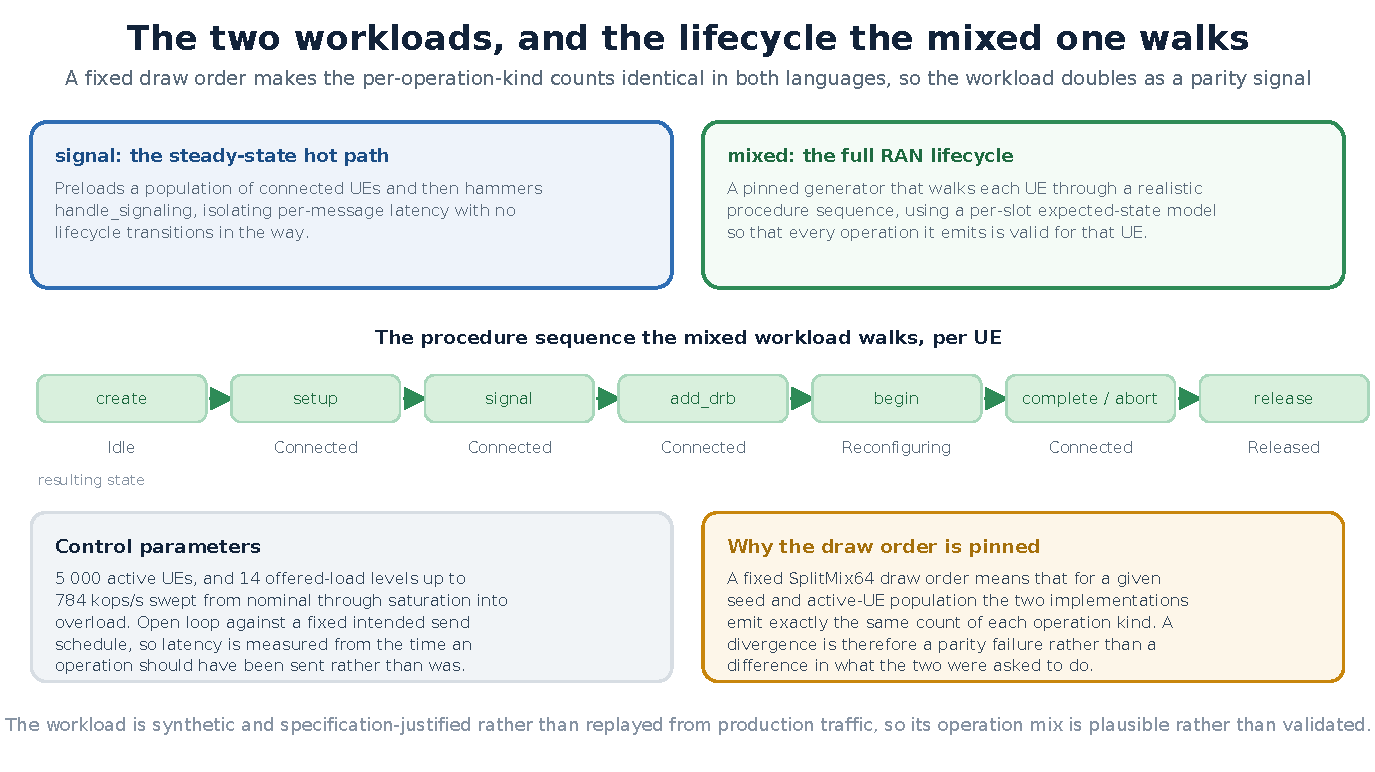
\includegraphics[width=0.78\linewidth]{diagrams/pdf/27_workload_timeline.pdf}
\caption[Hai workload và vòng đời workload mixed đi qua]{Hai workload. Workload \emph{signal} cô lập đường nóng ổn định.
Workload \emph{mixed} đi mỗi UE qua toàn chuỗi thủ tục RAN, với
mô hình trạng thái mong đợi theo slot đảm bảo mọi thao tác phát ra hợp pháp với trạng thái
ngữ cảnh thực sự ở. Vì thứ tự vẽ SplitMix64 được ghim, seed và
quần UE hoạt động cho trước tạo số đếm theo loại thao tác giống hệt ở cả hai ngôn ngữ, nên
phân kỳ là thất bại parity chứ không phải khác biệt trong việc hai triển khai được
yêu cầu làm.\label{fig:workload}}
\end{figure}

\paragraph{``Có căn đặc tả'' khẳng định gì, và không khẳng định gì.}
Thuật ngữ được dùng chính xác, vì phân biệt giới hạn workload hỗ trợ gì. \emph{Chuỗi}
thao tác được biện minh. Đó là vòng đời kết nối RRC mà đặc tả 3GPP
định nghĩa cho UE, từ thiết lập qua signalling trong phiên và thiết lập bearer
đến reconfiguration và release~\cite{3gpp38401,3gpp38331}. Mô hình trạng thái mong đợi theo slot sau đó
đảm bảo mọi thao tác driver phát ra hợp pháp với trạng thái ngữ cảnh thực sự ở,
nên workload không đẩy dịch vụ xuống đường đặc tả cấm. \emph{Tỷ lệ}
không được biện minh cùng cách. Tần suất cell thực handover so với
thiết lập bearer phụ thuộc triển khai, mobility, và thời điểm trong ngày, và không
có số công khai cố định. Mix dùng ở đây do đó hợp lý chứ không được xác thực.
Mục~\ref{sec:threats} báo đó là mối đe dọa tính ngoại sinh, và replay trace đứng đầu
danh sách công việc tương lai vì lý do này.

Với câu hỏi \emph{so sánh}, phân biệt ít tốn hơn so với câu tuyệt đối,
và nói vì sao là phần lập luận dữ liệu phù hợp nhiệm vụ. Cả hai triển khai thực thi
cùng chuỗi cùng thứ tự cho seed và quần UE hoạt động cho trước, và
số đếm theo loại thao tác xác minh. Mix không đại diện do đó dịch chuyển cả hai ngôn ngữ
bằng nhau và không thể tạo khác biệt giữa chúng. Mix thao tác chưa xác thực giới hạn số
đi xa bao nhiêu. Nó không làm suy yếu công bằng của so sánh chúng được dùng tạo.

Bảng~\ref{tab:params} gom cấu hình dịch vụ, workload và chiến dịch ở
một chỗ. Các giá trị đó nếu không gom sẽ rải qua đặc tả,
Chương~\ref{chapter:design}, và chương này. Tiện khi đọc từng phần, và
khó cho ai muốn tái lập chiến dịch hoặc đánh giá tham số có chọn để
phù hợp kết quả. Mỗi mục trong khối chiến dịch hoặc cố định bởi đặc tả hoặc
tạo từ log đo, nên không phần nào lệch khỏi dữ liệu báo cáo
dưới đây. Hai giá trị suy ra được dùng xuyên suốt phần sau. Điểm vận hành đại diện
không chọn bằng mắt. Nó là tải sweep bận nhất mà cả bốn variant build vẫn giữ
p99 dưới $5$~ms, đặt nó ở $\ReprLoad$~kops/s, so với bão hòa đo
$\SatKnee$~kops/s.

\section{Dữ liệu đánh giá}
Ba chiến dịch tạo ba tập dữ liệu, và chúng khác loại chứ không chỉ nội dung. Phần
sau mô tả mỗi tập khi được ghi. Người đọc đánh giá phân tích có đúng cần
biết gì được ghi và ở mức chi tiết nào, không chỉ gì được báo. Mọi đại lượng đo
chương này trích dẫn đến trang là macro được tạo.
\texttt{bench/refresh\_thesis.sh} tái tạo tất cả, cùng mọi hình và thân bảng,
từ log thô, nên rerun di chuyển văn bản và không thể để số tiêu đề
bị bỏ lại. Proxy chất lượng
phần mềm không thu ở đây mà báo nơi đọc rõ nhất: cạnh log điểm bắt buộc nó giải thích (Bảng~\ref{tab:complexity}), và cạnh seam FFI, nơi duy nhất
một trong hai triển khai chứa \texttt{unsafe} (Bảng~\ref{tab:ffi}).

\paragraph{Sweep hiệu năng.}
Mỗi trong $\NRuns$ lần chạy của thiết kế factorial Bảng~\ref{tab:params} đóng góp một
bản ghi, viết dạng JSON newline-delimited. Chiến dịch do đó là log append-only chứ không phải
bảng tóm tắt. Không gì được gộp khi ghi, và mọi statistic chương này được
tính lại từ bản ghi thô. Bản ghi mang cấu hình lần chạy (ngôn ngữ, bộ cấp phát,
workload, số shard và producer, tốc độ mục tiêu), kết quả (thao tác hoàn tất, lỗi,
thời lượng wall-clock, throughput đạt), phân phối độ trễ đọc từ histogram HDR
(mean, p50, p90, p99, p99.9, maximum, nanosecond), counter tài nguyên qua
\texttt{getrusage} (peak RSS, giây CPU user và system, mức
sử dụng CPU), và số đếm theo loại thao tác. Giữ số đếm loại trong mọi bản ghi là
điều làm phân kỳ giữa hai ngôn ngữ hiện là thất bại parity
(Mục~\ref{sec:parity}) thay vì bị nhầm là khác biệt hiệu năng.

\paragraph{Phân rã thành phần và nguyên thủy tranh chấp.}
Cấp đo thứ hai Mục~\ref{sec:methodperf} cho tập dữ liệu nhỏ hơn nhiều, hình dạng
khác. Với mỗi trong \BudgetRepeats{} lần lặp xen kẽ nó ghi chi phí batch-mean
ở cả hai ngôn ngữ, một lần gọi thao tác trực tiếp và một lần cùng thao tác qua
dịch vụ có luồng. Tập thứ ba, cùng hình ghép qua \ContentionRepeats{} lần lặp, ghi
throughput bền vững qua hàng đợi có giới hạn và nguyên thủy hoàn tất riêng
(Mục~\ref{sec:contention}). So sánh FFI Mục~\ref{sec:migrationresults} có
cùng cấu trúc qua \FfiOpRepeats{} lần lặp. Cả ba được ghép theo cấu trúc, điều test ghép chính xác
Mục~\ref{sec:stats} yêu cầu.

\paragraph{Catalogue tiêm lỗi.}
Tập dữ liệu này là phân loại chứ không số. Mỗi trong $\FaultClasses$ trường hợp lỗi cho bốn
log
công cụ: output AddressSanitizer, ThreadSanitizer và UndefinedBehaviorSanitizer cho chương trình C++,
và output \texttt{rustc} cho bản Rust an toàn tương ứng. Mỗi trường hợp cũng cho một
dòng taxonomy máy đọc được, ghi ba kết quả sanitiser, giai đoạn phát hiện,
kết quả compiler với mã chẩn đoán kích hoạt, và kỳ vọng đăng ký trước
nghiên cứu. Hai trường hợp boundary gốc cho bảng thứ hai từ model checker, và
\texttt{unsafe} một bảng thứ ba từ interpreter. Mang
kỳ vọng trong dữ liệu thay vì trong văn bản là điều cho runner báo mismatch
theo cả hai chiều. Bảng và hình Mục~\ref{sec:safetyresults} được tạo từ
file đó, không chép từ nó.

\paragraph{Điều đi cùng dữ liệu.}
Mỗi chiến dịch viết bản ghi môi trường cạnh kết quả. Nó ghi host và kernel,
distribution, phiên bản compiler và toolchain, mô hình CPU và topology, và governor tần số,
turbo, và cài đặt simultaneous-multithreading, \emph{kể cả} trường host cho trước
không expose. Chi tiết cuối quan trọng hơn nghe. Bản ghi xác định host
là guest KVM, và governor và turbo được lưu unavailable thay vì bỏ
đi. Hạn chế Mục~\ref{sec:testbed} tài liệu do đó là tính chất của tập dữ liệu
chứ không chỉ văn bản mô tả, và người đọc có thể kiểm tra không cần tin.

Tập dữ liệu hiệu năng đầy đủ và tự nhất quán cho phân tích và được dùng dưới đây để
trả lời RQ1 và RQ3 tạm thời. Chạy lại cùng script trên chiến dịch ghi trên
máy bare-metal thay các số bằng số cấp testbed không thay đổi
phân tích.

\section{Kết quả đánh giá}
Kết quả an toàn và migration không phụ thuộc máy đo. Kết quả hiệu năng và
tài nguyên phụ thuộc, và Mục~\ref{sec:testbed} nêu máy đó mang và không mang gì.
Mọi hình và bảng dưới đây được đo trên nó trừ khi nói khác.

Kết quả đã giải quyết và chưa giải quyết được báo cạnh nhau. Nói ngay đầu cái nào là gì
ngăn kết quả null bị đọc như không có. Sáu phát hiện đã giải quyết: taxonomy
lớp lỗi và ranh giới (Mục~\ref{sec:safetyresults}), chi phí seam FFI
(Mục~\ref{sec:migrationresults}), khác biệt bộ nhớ giữa hai build
(Mục~\ref{sec:resources}), chi phí thao tác thuần (Mục~\ref{sec:budget}), tương đương bốn variant ở median dưới bão hòa, và phân kỳ qua nó
(Mục~\ref{sec:overload}). Cái cuối là hiệu ứng ngôn ngữ lớn nhất và tái lập nhất
trong nghiên cứu.

Đuôi xa \emph{dưới} bão hòa là kết quả chưa giải quyết duy nhất, và host là lý do.
Spread run-to-run ở p99 vượt mọi khác biệt giữa variant, và không số lần lặp
trên máy ảo với CPU steal khác không đóng khoảng đó
(Mục~\ref{sec:perfresults}). Chỉ protocol bare-metal Mục~\ref{sec:testbed} sẽ
trả lời. Phân kỳ quá tải được giải quyết như phép đo, dù chưa đầy như cơ chế.
Mục~\ref{sec:contention} kiểm tra hàng đợi có giới hạn và nguyên thủy hoàn tất riêng
có giải thích không. Chúng không tái tạo thứ tự full-service ở mức ý nghĩa, để lại
việc ở đâu đó trên toàn đường handoff ngoài nguyên thủy cô lập.

\subsection{Hiệu năng (RQ1, RQ3)}\label{sec:perfresults}
Giả thuyết được thử là H1: hai ngôn ngữ tương đương hiệu năng dưới
bão hòa, mọi khác biệt chỉ ở đuôi xa. Mục này báo nơi, nếu
có, mỗi bên thắng và bao nhiêu, qua sweep tới và qua bão hòa.

Mọi thứ trong mục được tạo từ log thô bởi \texttt{bench/plot\_figures.py}: hình,
bảng, và số trích trong văn bản. Mục do đó có thể tái tạo
nguyên văn nếu chiến dịch rerun trên testbed bare-metal. Số tuyệt đối thuộc
host Mục~\ref{sec:testbed}. Mỗi điểm gộp \NRepeats{} lần lặp xen kẽ.
Giá trị bảng và dải shaded là median với khoảng tin cậy bootstrap $95\%$
nonparametric.

Bảng~\ref{tab:latency} tóm tắt phân phối độ trễ mỗi thao tác ở tải đề nghị
bền vững $\ReprLoad$~kops/s. Điểm vận hành không chọn bằng mắt: nó là
tải sweep cao nhất mà mọi một trong bốn variant build vẫn giữ p99 dưới
$5$~ms, tức điểm bận nhất mà cả bốn cùng khỏe, làm
nó nơi công bằng nhất để so sánh.

Bảng phải đọc ở hai mức tin cậy khác nhau, và tách chúng là
cách đọc trung thực của chiến dịch. Ở \emph{median} bốn variant nằm trong
$\PFiftyRange\,\mu$s của nhau, hay $\PFiftySpread\%$, và mọi cặp khoảng tin cậy
giao nhau. Bảng đơn lẻ do đó không phân tách gì.
Đó là câu về khoảng không ghép chứ không về ngôn ngữ. Test ghép
dưới đây giải quyết khác biệt nhỏ và nhất quán ở median, và khoảng giữa
hai cách đọc chính xác là lý do Mục~\ref{sec:stats} test so sánh thay vì
nhìn khoảng.

\emph{Trên} median tình huống khác loại. Điểm không phải ngôn ngữ khác mà host này không thể nói có khác không. Giá trị p99 khác
$\PNineNineRange\,\mu$s giữa variant, trong khi khoảng tin cậy $95\%$ rộng nhất trên
p99 của một variant đơn trải $\PNineNineMaxCI\,\mu$s, nhiều lần khác biệt
giữa variant. Khi uncertainty về một variant vượt khoảng giữa cả bốn, không
thứ tự nào đọc được. Báo một sẽ là báo scheduler. Cùng điều
mạnh hơn ở p99.9 và maximum.

Đây là dạng cụ thể của hạn chế Mục~\ref{sec:testbed} nêu, và chi phí được
giới hạn. Nó không chạm throughput và hành vi bão hòa, kết quả tài nguyên dưới đây,
hay gì trong chương RQ2 và RQ4. Nó nghĩa là một nửa RQ1 chỉ nhận
câu trả lời phủ định từ chiến dịch này, tức hai ngôn ngữ hành xử thế nào ở percentile cao
khi dịch vụ vẫn đáp ứng tải đề nghị. Đuôi đó chưa đo được. Nửa kia
không bị chạm, và Mục~\ref{sec:overload} giải quyết nó dứt khoát trên cùng host này.
Đóng khoảng cần protocol bare-metal, không thêm lần lặp ở đây, vì spread là
nhiễu hệ thống chứ không phải nhiễu lấy mẫu. Mục~\ref{sec:budget} cũng cho thấy
đại lượng ngôn ngữ có thể ảnh hưởng nằm hơn ba bậc magnitude dưới đại lượng
phép đo này giải quyết.

Một điều chỉnh về metric thuộc đây chứ không chỉ thảo luận tính hợp lệ. RQ1
nêu median, p99, p99.9, và maximum vì bốn đó là chiến dịch này cung cấp.
Harness cũng ghi jitter giữa thao tác và p99.99, và giữ histogram đuôi xa
sẽ phải gộp từ, nhưng chiến dịch báo ở đây trước instrumentation đó.
Khả năng dự đoán do đó được chứng minh ở p99 và p99.9 và không xa hơn. Đó là khoảng trong
bằng chứng chứ không trong thiết kế, và nó đóng với chiến dịch bare-metal mà luận điểm đuôi
đã chờ.

\begin{table}[H]
\centering
\small
\caption[Độ trễ mỗi thao tác ở tải đại diện]{Độ trễ mỗi thao tác ở tải đề nghị bền vững $\ReprLoad$~kops/s (workload
vòng đời RAN mixed, $7$ shard). Giá trị microsecond: median qua \NRepeats{}
lần lặp trên khoảng tin cậy bootstrap $95\%$ nonparametric. Khoảng in đầy đủ thay vì nửa rộng đối xứng vì nó
rất bất đối xứng ở các percentile này, và nửa rộng đủ che bound trên sẽ đặt bound dưới
dưới không.\label{tab:latency}}
% Tabular preamble and header are generated alongside the table body, so the table
% gains a p99.99 column when a campaign records one instead of the preamble falling
% one column short of the body it is wrapping. \LatencyTabular expands to the whole
% \begin{tabular}{...}: array's preamble scanner does not expand macros, so passing
% only the column specification would fail with "Illegal pream-token".
\LatencyTabular
\hline\hline
\LatencyHead \\
\hline
C++ (system alloc) & \mci{217.2}{163.8}{237.2} & \mci{355.1}{289.3}{389.4} & \mci{674.3}{395.3}{1538.0} & \mci{2170}{910}{5594} \\
C++ (jemalloc) & \mci{225.8}{181.1}{261.2} & \mci{410.1}{305.7}{11280.4} & \mci{1188}{544}{14213} & \mci{3590}{1472}{16291} \\
Rust (system alloc) & \mci{214.3}{191.6}{238.8} & \mci{376.3}{330.2}{3629.1} & \mci{1068}{504}{6955} & \mci{2404}{1129}{9667} \\
Rust (jemalloc) & \mci{208.4}{193.7}{223.1} & \mci{388.9}{342.3}{478.0} & \mci{763.4}{479.5}{4272.1} & \mci{2804}{1114}{7606}
\\
\hline
\end{tabular}
\end{table}

\paragraph{Test so sánh thay vì nhìn mắt.}
Khoảng giao nhau là công cụ yếu theo cả hai chiều, nên so sánh cũng được test
trực tiếp, theo thủ tục cố định Mục~\ref{sec:stats} và báo trong
Bảng~\ref{tab:significance}. Điều cho phép ghép là tính chất của chiến dịch này chứ
không của statistic. Bốn variant được xen kẽ trong mỗi lần lặp, nên
lần chạy $i$ của mỗi được đo trong cùng block dưới cùng điều kiện môi trường. Mọi
nhiễu block mang là chung cho cặp, và hủy trong hiệu của chúng. Đó là
thứ hai kỷ luật xen kẽ mua, ngoài lập luận công bằng nó được chọn
vì.

\begin{table}[tp]
\centering
\small
\caption[Test ghép hoán vị chính xác C++ so với Rust]{Test ghép hoán vị chính xác C++ so với Rust ở $\ReprLoad$~kops/s, với
bộ cấp phát giữ cố định. Hiệu ứng là median của \NRepeats{} hiệu ghép
(Rust~$-$~C++), hiển thị trên khoảng tin cậy bootstrap $95\%$. Statistic test là
mean của chúng. $p$ chính xác qua mọi $2^{\NRepeats}$ gán dấu, và cột cuối
áp dụng hiệu chỉnh Holm trên cả họ \NTests{} test. Sàn có thể đạt
là $\MinAttainableP$ chưa hiệu chỉnh và $\CorrectedFloor$ sau hiệu chỉnh. Các dòng được khối
theo tập tiêu chí Mục~\ref{sec:stats}: ghép cứu statistic ở khối trên, nên khoảng nhất quán ở đó là bằng chứng, trong khi percentile cao dưới được tính từ đúng thao tác nhiễu rơi vào, nên khoảng loại trừ không được đọc là phát hiện. Throughput đạt không được test, vì lý do
cùng mục, và xuất hiện trong Bảng~\ref{tab:resource}. Đo trên host Xeon ảo
Mục~\ref{sec:testbed}.\label{tab:significance}}
\begin{tabular}{@{}l l r r r@{}}
\hline\hline
Metric & Allocator & Effect (Rust $-$ C++) & $p$ & Holm \\
\hline
\rlap{\emph{Robust to interference on single operations}} & & & & \\
p50 latency (\textmu s) & system & \mci{-1.3}{-1.3}{-1.2} & 0.0000019 & 0.000027 \\
p50 latency (\textmu s) & jemalloc & \mci{-1.2}{-1.3}{-1.2} & 0.0000019 & 0.000027 \\
Peak RSS (MiB) & system & \mci{+1.4}{+1.2}{+1.7} & 0.0000019 & 0.000027 \\
Peak RSS (MiB) & jemalloc & \mci{+2.5}{+2.4}{+2.6} & 0.0000019 & 0.000027 \\
CPU utilisation (\%) & system & \mci{-5.1}{-6.7}{-4.7} & 0.0000019 & 0.000027 \\
CPU utilisation (\%) & jemalloc & \mci{-4.6}{-5.9}{-3.9} & 0.0000019 & 0.000027\\
\hline
\rlap{\emph{Determined by it: high percentiles}} & & & & \\
p99 latency (\textmu s) & system & \mci{-1}{-2}{-1} & 0.0000057 & 0.000027 \\
p99 latency (\textmu s) & jemalloc & \mci{-1}{-1}{-1} & 0.0000038 & 0.000027 \\
p99.9 latency (\textmu s) & system & \mci{-4}{-5}{-2} & 0.00016 & 0.00016 \\
p99.9 latency (\textmu s) & jemalloc & \mci{-2}{-4}{-2} & 0.0000095 & 0.000027
\\
\hline
\end{tabular}
\end{table}

\begin{figure}[ht]
\centering
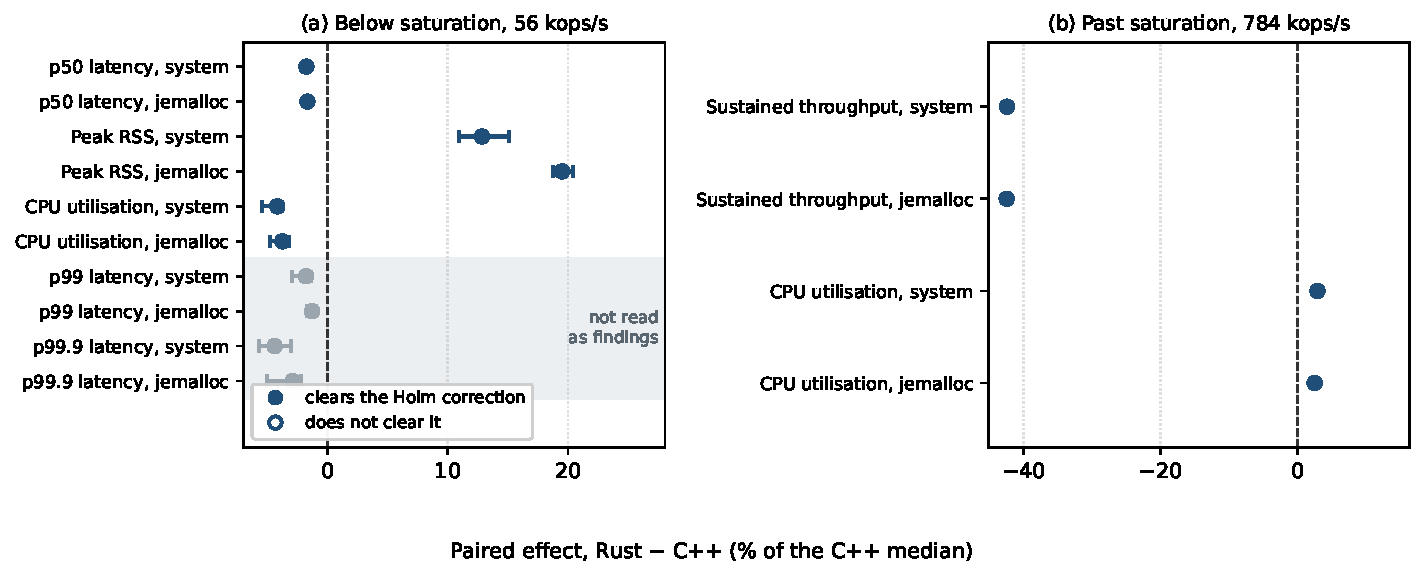
\includegraphics[width=0.78\linewidth]{figures/fig_effects.pdf}
\caption[Họ test được vẽ dưới dạng hiệu ứng ghép]{Mọi test trong Bảng~\ref{tab:significance} và~\ref{tab:overloadtest} dưới dạng hiệu ứng
ghép với khoảng bootstrap $95\%$, chuẩn hóa theo median C++ để microsecond,
mebibyte, điểm phần trăm và kops/s chia sẻ trục. Marker đầy là
\NSignificant{} trong \NTests{} test vượt hiệu chỉnh Holm. Hai bộ cấp phát của
metric được vẽ cạnh nhau, nên hiệu ứng đổi dấu giữa chúng sẽ hiện là cặp
qua đường không. Các dòng shaded là percentile cao, tính từ đúng thao tác nhiễu rơi vào, mà Mục~\ref{sec:stats} cố định trước là dòng có khoảng
không đọc là phát hiện. Metric giữ đơn vị riêng trong
bảng.\label{fig:effects}}
\end{figure}

Hình~\ref{fig:effects} vẽ cùng họ trên một trục, và ba điều trong đó
dễ thấy hơn trong bảng mười bốn dòng: hiệu ứng nào sống sót hiệu chỉnh,
hiệu ứng có giữ dấu khi bộ cấp phát đổi không, và khoảng đuôi
rộng hơn phần còn lại bao nhiêu.

Năm điều theo sau. Thứ nhất, \NSignificant{} trong \NTests{} test của họ sống sót hiệu chỉnh
Holm. Ở điểm vận hành này chúng là hai dòng median-latency, peak RSS
dưới bộ cấp phát hệ thống, và cả hai dòng CPU. Bốn còn lại sống sót là so sánh quá tải
Mục~\ref{sec:overload}. Peak RSS dưới jemalloc là dòng
khối trên duy nhất không vượt hiệu chỉnh, dù khoảng xa không, và
Mục~\ref{sec:resources} nói vì sao.

Thứ hai, quy tắc đọc cố định Mục~\ref{sec:stats} phải áp dụng trước khi diễn giải bất kỳ. \NExclZero{} khoảng ghép loại trừ không. Trong khối đuôi những loại trừ là: \TailExclZeroRows. Quy tắc được nêu trước, và không ở điểm này, chính xác
vì kết quả đó không được đảm bảo. Lượt trước bảy lần lặp cùng chiến dịch
đã tạo khoảng đuôi loại trừ không, và thêm lần lặp sau đó gỡ chúng. Đó là hành vi
quy tắc dự đoán.

Thứ ba, đối chứng bộ cấp phát cung cấp kiểm tra thứ hai, độc lập với thứ nhất. Mọi so sánh
chạy hai lần dưới điều kiện không nên đổi hiệu ứng ngôn ngữ, nên hiệu ứng thực sự
là ngôn ngữ nên giữ dấu dù liên kết bộ cấp phát nào. Ở đây
\CrossAllocConsistent{} tất cả giữ, và \NCrossAllocReversed{} đảo. Đối chứng xác nhận thay vì
phủ quyết không phải bằng chứng nó không cần. Trong chiến dịch trước, trước khi hai build \texttt{jemalloc} bị giữ một cấu hình, hiệu ứng CPU vượt hiệu chỉnh
dưới một bộ cấp phát và đảo dấu dưới bộ kia, và được báo chưa giải quyết theo
chính quy tắc này. Đối chứng kiếm chỗ bằng điều nó sẽ bắt, không phải điều nó
tình cờ bắt.

Thứ tư, \NEqvUnresolved{} dòng hiệu chỉnh không vượt không nói cùng một điều, và Bảng~\ref{tab:equivalence} là thứ tách chúng. Test không giải quyết khác biệt vẫn giới hạn nó: có margin chặt nhất trong đó hai variant có thể
gọi tương đương, và đó là tính chất dữ liệu chứ không phán quyết. Đọc vậy
khối trên và khối đuôi tách rõ. Ở median bound là
$\EqvBoundPFifty\,\mu$s, nên khác biệt test giải quyết cũng nhỏ theo tuyệt đối
và hai cách đọc đồng ý. Trong khối đuôi bound chạy tới $\EqvBoundTailMax\,\mu$s,
là khả năng host này không nhìn thấy được nêu dưới dạng số thay vì null. Phân biệt
quan trọng vì hai thứ thường được báo giống. Null với bound chặt là
kết quả. Null với bound rộng hơn mọi khác biệt triển khai quan tâm là
chiến dịch từ chối trả lời, và nói cái nào là điều tối thiểu bảng này làm cho nửa RQ1 host không thể giải quyết.

\begin{table}[H]
\centering
\small
\caption[Mỗi hiệu ứng có thể lớn bao nhiêu, cho so sánh test không giải quyết]{Mỗi hiệu ứng có thể lớn bao nhiêu. Với mọi so sánh ở $\ReprLoad$~kops/s,
hiệu ứng quan sát so với margin chặt nhất trong đó hai variant có thể gọi
tương đương, và phán quyết Bảng~\ref{tab:significance} đạt. Hai câu hỏi
cố ý giữ ở hai bảng: một hỏi khác biệt có ở đó không, bảng này hỏi nó
có thể lớn bao nhiêu nếu có, và một dòng có thể quan trọng ở một mà không ở bảng kia. Margin độ trễ là
microsecond, peak RSS mebibyte, sử dụng CPU điểm phần
trăm.\label{tab:equivalence}}
\begin{tabular}{@{}l l r r l@{}}
\hline\hline
Metric & Allocator & $|$Effect$|$ & Equivalent within & Verdict \\
\hline
p50 latency (\textmu s) & system & 1.2 & 1.3 & significant \\
p50 latency (\textmu s) & jemalloc & 1.5 & 1.6 & significant \\
p99 latency (\textmu s) & system & 2 & 2 & significant \\
p99 latency (\textmu s) & jemalloc & 1 & 1 & significant \\
p99.9 latency (\textmu s) & system & 4 & 4 & significant \\
p99.9 latency (\textmu s) & jemalloc & 3 & 3 & significant \\
Peak RSS (MiB) & system & 1.6 & 1.8 & significant \\
Peak RSS (MiB) & jemalloc & 2.5 & 2.5 & significant \\
CPU utilisation (\%) & system & 6.0 & 7.1 & significant \\
CPU utilisation (\%) & jemalloc & 6.2 & 7.3 & significant
\\
\hline
\end{tabular}
\end{table}

Thứ năm, median giờ là khác biệt đã giải quyết chứ không phải null: $\PFiftyDiffAbsMax\,\mu$s
theo hướng có lợi Rust, nhất quán dưới cả hai bộ cấp phát. Khoảng trên nó chạm
$\PFiftyDiffCIMax\,\mu$s so với median khoảng $80\,\mu$s, và cám dỗ là báo
đó là bound trên hiệu ứng ngôn ngữ. Cách đọc đó sai, và mục
sau giải thích vì sao.

\subsection{End-to-end số được ghép từ gì}\label{sec:budget}
Mọi độ trễ sweep báo là vòng quay end-to-end, và
Mục~\ref{sec:methodperf} nêu vì sao đó gói hai chi phí khác loại.
Một là thao tác, thực thi trong một luồng và do compiler tạo. Cái kia
là handoff gửi-và-hoàn tất qua luồng, tính cho hệ điều hành.
Chỉ cái đầu có thể khác giữa ngôn ngữ, và sweep không tách hai.

Điều quan trọng cho bound vừa trích, vì bound chỉ nói bằng đại lượng
nó là phần của. Cả hai chi phí do đó được đo trực tiếp, bằng phương pháp hai cấp
mô tả ở đó, ở cả hai ngôn ngữ và ở số shard và quần ngữ cảnh của sweep.
\texttt{ShardCore} gọi không có hàng đợi trên đường cho thao tác. \texttt{Service} cho
thao tác cộng handoff. Hiệu của chúng là handoff.
Bảng~\ref{tab:budget} cho kết quả, và nó định hình lại toàn so sánh hiệu năng.

\begin{table}[H]
\centering
\small
\caption[Chi phí end-to-end thực sự đi đâu]{Chi phí end-to-end thao tác thực sự đi đâu, đo ở $7$ shard và
$5\,000$ UE hoạt động với một caller không tranh chấp. Mỗi dòng là median qua
\BudgetRepeats{} lần lặp xen kẽ trên khoảng tin cậy bootstrap $95\%$, theo
đơn vị magnitude gọi: hai thành phần khác hơn hai bậc magnitude,
điểm của bảng. $p$ là test ghép hoán vị hai phía chính xác C++
so với Rust trên hiệu theo lần lặp. Handoff có bằng hiệu hai dòng
đo, nên mang uncertainty của cả hai.\label{tab:budget}}
\begin{tabular}{@{}l r r r@{}}
\hline\hline
Thành phần & C++ & Rust & $p$ \\
\hline
Operation alone, no queue in the path (ns) & \mci{34.4}{32.5}{34.5} & \mci{21.3}{21.0}{22.5} & 0.000061 \\
Cross-thread submit-and-complete handoff (\textmu s) & \mci{13.49}{13.36}{13.64} & \mci{12.61}{12.37}{12.89} & 0.227 \\
End-to-end round-trip, uncontended (\textmu s) & \mci{13.52}{13.39}{13.68} & \mci{12.63}{12.39}{12.91} & 0.215 \\
Operation's share of the round-trip & 0.250\,\% & 0.170\,\% & 
\\
\hline
\end{tabular}
\end{table}

Thao tác là $\BudgetCoreCpp$~ns trong C++ và $\BudgetCoreRust$~ns trong Rust. Handoff là
$\BudgetHandoffCpp\,\mu$s và $\BudgetHandoffRust\,\mu$s. Việc ngôn ngữ thực sự
làm chiếm tối đa $\BudgetCoreShareMax\%$ của sweep đo. Phần
bù $\BudgetCoreShareRest\%$ của mọi độ trễ Bảng~\ref{tab:latency} là hệ điều hành di chuyển thông điệp giữa hai luồng.

Hình dạng đó không đặc thù hệ này hay cặp ngôn ngữ này. Zhou et al.\ xem lại
phân rã kinh điển chi phí xử lý giao dịch trên database shared-nothing, xây như
dịch vụ này với một partition mỗi worker thread. Sau khi việc mỗi thao tác được
tối ưu, họ báo phần còn lại chủ yếu là giao tiếp qua
ranh giới cô lập chứ không phải thao tác~\cite{zhou2025oltp}. Bảng trên là
cùng mẫu trong dịch vụ control-plane, làm kết quả dưới đây tính chất chung của thiết kế chứ không artefact của phép đo.

Hai kết luận theo sau, và chúng kéo ngược chiều.

Thứ nhất, sweep không thể bound hiệu ứng ngôn ngữ, và bound trên không được
đọc như nó bound. Khoảng $\PFiftyDiffCIMax\,\mu$s trên hiệu median ghép
là $\BudgetBoundVsCore$ lần chi phí riêng của thao tác. Hiệu ứng ngôn ngữ có thể
vài trăm phần trăm việc đang làm và vẫn nằm gọn trong nó. Sweep
thiết lập yếu hơn và vẫn hữu ích: không ngôn ngữ làm rối
vòng quay do scheduler chi phối, điều triển khai hình dạng này thực sự
trải nghiệm. Nó không thể thiết lập gì về mã compiler phát ra. Giới hạn đó đến từ cách phép đo được xây chứ không từ host,
nên không như kết quả đuôi sẽ không sửa bằng chuyển bare metal. Nó được sửa bằng
đo thành phần riêng, điều mục này làm.

Thứ hai, một khi thành phần \emph{được} đo riêng, ngôn ngữ không
tương đương. \BudgetCoreFaster{} chạy thao tác thuần nhanh hơn khoảng $\BudgetCoreRatio\times$,
khác biệt xuất hiện ở đại đa số lần lặp, và test ghép đặt nó hai
bậc magnitude dưới ngưỡng thông thường. Phân rã này là thí nghiệm
riêng so với sweep và không phần của họ Holm. Nó chạy \BudgetRepeats{} lần lặp
thay vì \NRepeats{}, nên sàn có thể đạt riêng là $0.000061$ chứ không phải
$\CorrectedFloor$ trích Mục~\ref{sec:stats}, và không hiệu chỉnh áp dụng cho nó. Cùng điều cho so sánh interoperability Mục~\ref{sec:migrationresults}. Đây là
nơi duy nhất trong cả chiến dịch hiệu năng mà khác biệt ngôn ngữ trong \emph{thời gian} được giải quyết, và sweep mù với nó hơn
hai bậc magnitude.

Hình~\ref{fig:budget} vẽ cả hai kết luận trên một trang, vì mỗi cái dễ thấy hơn
đọc từ bảng số trải bốn decade. Panel thứ hai là lập luận mục
này: công cụ nằm hoàn toàn trên đại lượng nó phải ràng buộc.

\begin{figure}[ht]
\centering
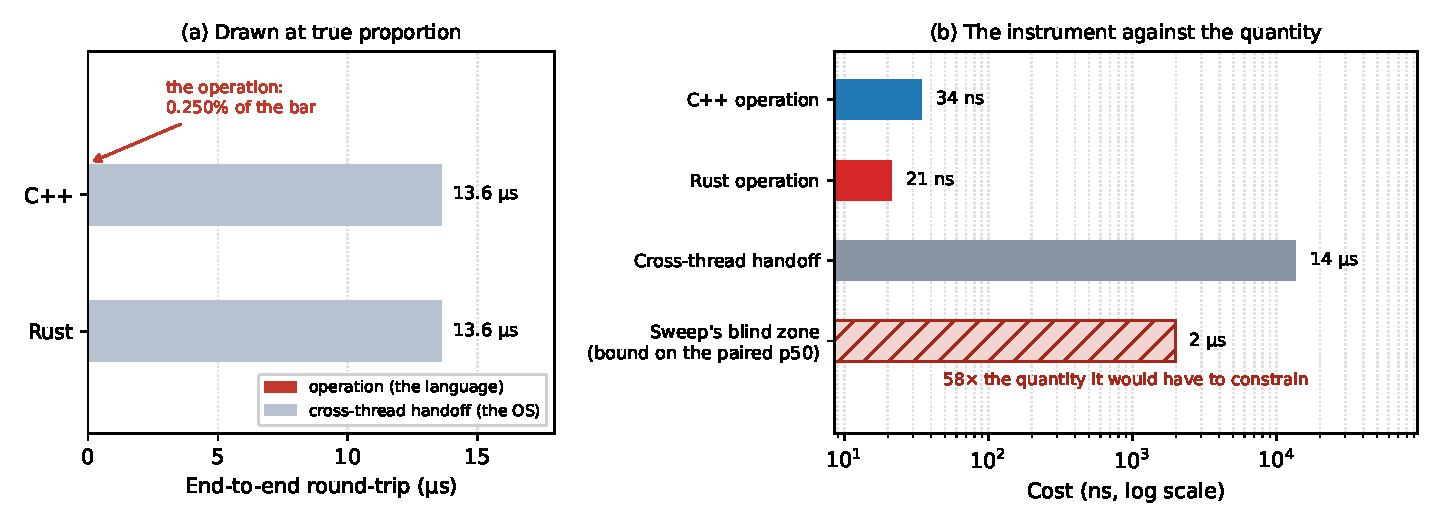
\includegraphics[width=0.78\linewidth]{figures/fig_budget.pdf}
\caption[Thao tác end-to-end được phân rã, so với sweep có thể giải quyết]{Chi phí end-to-end thao tác đi đâu, và vì sao sweep không bound hiệu ứng
ngôn ngữ. \textbf{(a)} Vòng quay theo tỷ lệ thật: thao tác ngôn ngữ thực hiện là
$\BudgetCoreShareMax\%$ thanh, phần còn lại handoff qua luồng. \textbf{(b)} Cùng đại lượng trên trục log so với hiệu ghép nhỏ nhất sweep có thể giải quyết,
hiển thị là vùng mù. Cả hai phép đo thao tác nằm trong nó bằng hệ số
$\BudgetBoundVsCore$, và (b) cũng là nơi khác biệt thời gian duy nhất chiến dịch giải quyết
nằm.\label{fig:budget}}
\end{figure}

Gán nhận cần cẩn thận, vì cách đọc tự nhiên là sai. Không gì ở đây
liên quan borrow checker, kiểm tra bound, hay ownership. Nguồn có thể nhất
đã ghi trong log điểm bắt buộc Bảng~\ref{tab:idioms}. Container mỗi shard là
hash map chuẩn của mỗi ngôn ngữ, và chúng là cấu trúc dữ liệu khác. \texttt{std::unordered\_map} của C++ phải node-based để giữ cam kết ổn định iterator và reference,
nên lookup đuổi pointer từ mảng bucket ra node cấp phát riêng. \texttt{HashMap} của Rust là bảng open-addressed giữ entry inline và
thường giải quyết lookup trong một cache line. Hàm hash được ghim FNV-1a cả hai
bên (Mục~\ref{sec:impldetails}) chính xác để hashing không thể là giải thích,
để lại bố cục container. Đó là khác biệt thật và có thể báo giữa hai
ngôn ngữ như thực tế dùng, vì developer chọn hash map chuẩn nhận
cái ngôn ngữ họ ship. Không phải bằng chứng về mô hình an toàn Rust và không
nên trích như vậy. Xác nhận cơ chế cần counter cache-miss
Mục~\ref{sec:threats} liệt kê là khoảng instrumentation rõ nhất.

Ba giới hạn giữ phát hiện đúng kích thước. Đó là microbenchmark một luồng, không tranh chấp,
nên nói thao tác tốn bao nhiêu chứ không hệ tải làm gì với nó. Đo trên cùng host sweep, nên số tuyệt đối mang cùng cảnh báo, dù tỷ số ít nhạy hơn mỗi thành phần. Và đó là một
thao tác trên một cấu trúc dữ liệu. Tổng quát hóa thành ``Rust nhanh $\BudgetCoreRatio\times$
hơn'' sẽ lặp chính lỗi luận văn này chỉ trích trong literature trường hợp trung bình.

\subsection{Độ trễ, throughput và bão hòa qua sweep}
Hình~\ref{fig:latency-load} vẽ p99 độ trễ so với tải đề nghị, và hình dạng là
hình Hình~\ref{fig:cliff} phác. Qua vùng tracking bốn variant leo
cùng nhau và nhẹ, từ khoảng $240\,\mu$s ở tải nhẹ tới single-digit millisecond
bởi $\SatKnee$~kops/s. Dải tin cậy ở đó đủ rộng để không curve tách
khỏi curve khác ở vùng đó. Sau đó, trong một bước duy nhất của thang tốc độ tiếp theo,
p99 mọi variant tăng hơn hai bậc magnitude cùng lúc, từ khoảng $6$~ms tới
vài giây. Đó là vách quá tải, và mức đột ngột đến là phát hiện. Một
bước tăng tải đề nghị tách dịch vụ đáp ứng deadline millisecond khỏi dịch vụ lỡ
ba bậc magnitude. Thiết kế với hàng đợi chặn có giới hạn không có suy giảm nhẹ nhàng
ở giữa.

Hai tính chất phía xa vách giới hạn ý nghĩa số, và chúng là lý do
Mục~\ref{sec:stats} không test percentile ở đó. Độ trễ qua knee là backlog
lịch tích chứ không phải thời gian phục vụ. Và vì giai đoạn đo bị cắt ở
chiều rộng cố định, percentile báo cáo bão hòa gần chiều rộng đó, làm mọi percentile
trên knee là bound dưới. Điều còn diễn giải được trong regime này là mỗi variant
vẫn hoàn tất bao nhiêu việc, và Mục~\ref{sec:overload} nói tiếp.

\begin{figure}[ht]
\centering
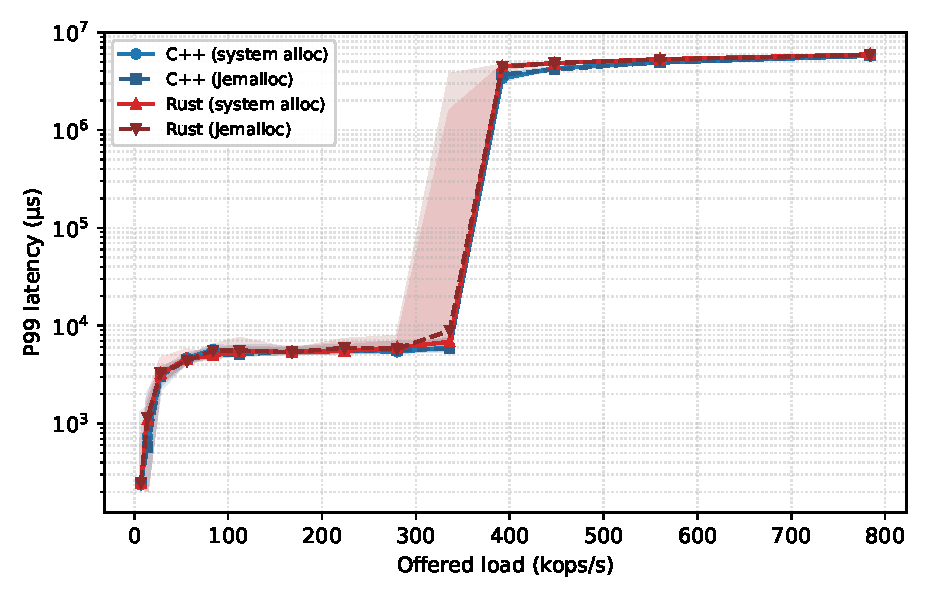
\includegraphics[width=0.66\linewidth]{figures/fig_latency_vs_load.pdf}
\caption[Độ trễ đuôi so với tải đề nghị]{Độ trễ đuôi (p99) so với tải đề nghị cho bốn variant build. Đường là median
qua \NRepeats{} lần lặp. Dải shaded là CI bootstrap $95\%$. Trục $y$ log.
\label{fig:latency-load}}
\end{figure}

Hình~\ref{fig:throughput-load} cho throughput đạt so với tải đề nghị, và là
plot thông tin hơn. Throughput là trung bình cả lần chạy, làm nó ít
nhạy hơn percentile với nhiễu rơi vào thao tác riêng lẻ.
Mọi variant bám đường lý tưởng đề nghị-bằng-đạt tới $\TrackingLoad$~kops/s và
bão hòa khoảng $\SatKnee$~kops/s. Hai điều theo ngay. Thứ nhất, throughput đạt
khớp tải đề nghị dưới knee trong $\ReprLoadShortfall\%$, nên điểm vận hành
Bảng~\ref{tab:latency} là tải \emph{bền vững} thật chứ không danh nghĩa.
Độ trễ báo ở đó không phải của hệ đã xếp hàng. Thứ hai, knee
nằm cùng chỗ cho cả bốn variant, điều cấu trúc một luồng mỗi shard
dự đoán. Nơi thiết kế không còn chịu là tính chất thiết kế.

Điều xảy ra \emph{sau} knee không được chia sẻ. Bốn curve tách ngay khi
tốc độ đề nghị không còn đáp ứng, và tách theo ngôn ngữ chứ không theo bộ cấp phát.
Mục~\ref{sec:overload} đo phân tách đó thay vì để mắt.

\begin{figure}[ht]
\centering
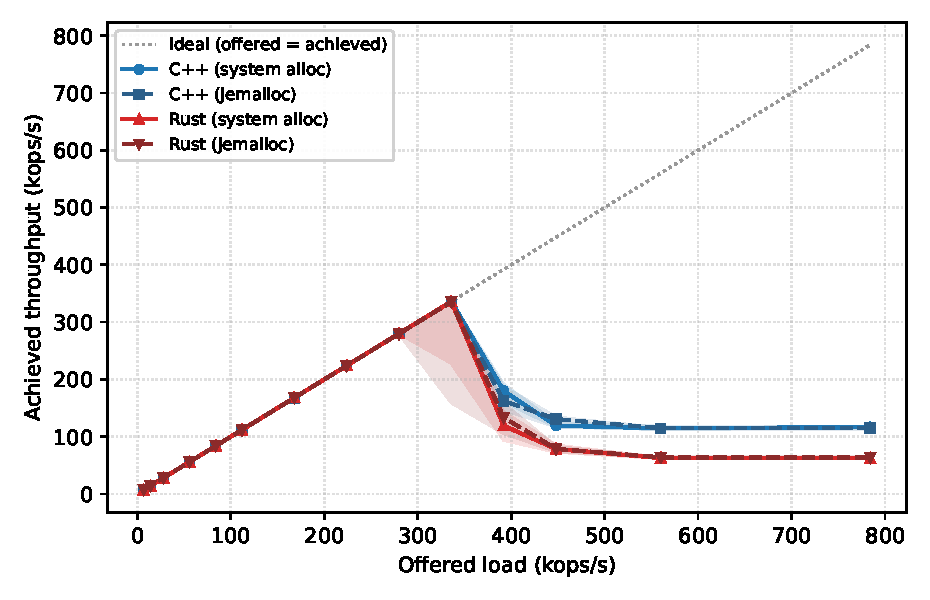
\includegraphics[width=0.66\linewidth]{figures/fig_throughput_vs_load.pdf}
\caption[Throughput đạt so với tải đề nghị]{Throughput đạt so với tải đề nghị. Đường chấm đánh dấu regime lý tưởng
đề nghị-bằng-đạt. Throughput được đếm chỉ trong giai đoạn đo, nên warm-up
không thiên cả mẫu số và tử số.\label{fig:throughput-load}}
\end{figure}

Hình~\ref{fig:tailpct} giữ tải cố định và sweep percentile. Bốn
variant trùng ở median và tỏ ra khi percentile tăng. Đó là hình dạng mong đợi
cho phân phối heavy-tailed, và là lý do methodology nhận biết percentile dùng xuyên suốt.
Tỏ ra không phải hiệu ứng ngôn ngữ, và panel phải cho thấy vì sao. Nó đặt spread
giữa bốn variant ở mỗi percentile so với khoảng rộng nhất một variant
mang ở đó. Ở median spread là lớn hơn của hai, regime
trong đó thứ tự có nghĩa. Từ p90 trở lên khoảng vượt spread nhiều lần. Sự tỏ ra do đó đánh dấu nơi phép đo mất độ phân giải, không nơi
ngôn ngữ khác.

\begin{figure}[ht]
\centering
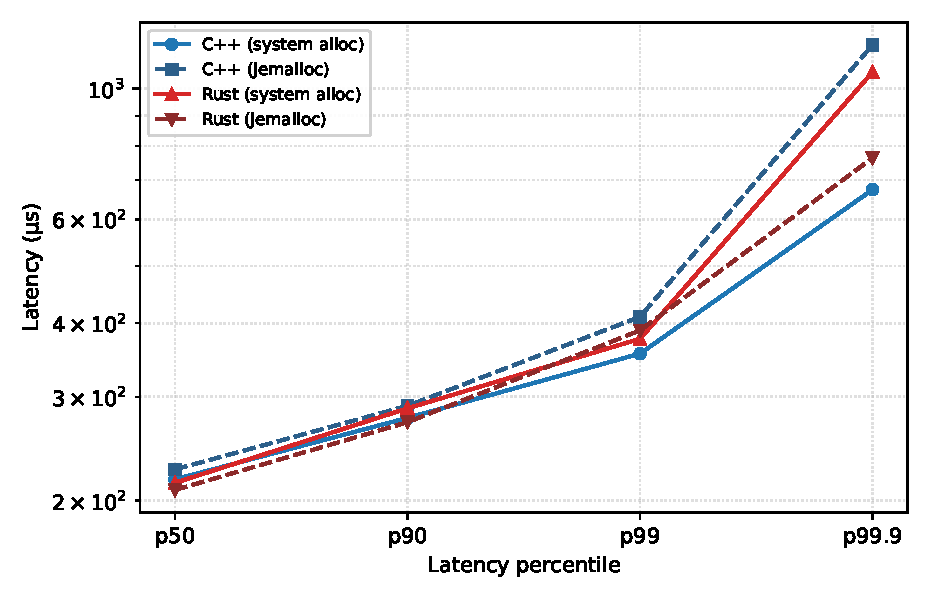
\includegraphics[width=0.78\linewidth]{figures/fig_tail_percentiles.pdf}
\caption[Độ trễ qua dải percentile, và giới hạn host]{Độ trễ mỗi thao tác qua dải percentile ở $\ReprLoad$~kops/s. \textbf{(a)} Bốn
variant là median qua \NRepeats{} lần lặp, mỗi cái với dải bootstrap $95\%$. Dải
là điểm: vẽ đường trần các curve chồng lên và đọc như tuyên bố
tương đương, không phải điều phép đo không thể tách đã chứng minh. \textbf{(b)}
Vì sao không thể tách trên median. Spread giữa bốn variant được đặt
so với khoảng tin cậy rộng nhất trên bất kỳ một variant, với tỷ số chú thích trên mỗi
cặp thanh. Khi tỷ số vượt một, uncertainty về một variant lớn hơn
khoảng giữa cả bốn và không thứ tự nào đọc được.\label{fig:tailpct}}
\end{figure}

\subsection{Hành vi qua bão hòa (RQ1)}\label{sec:overload}
RQ1 hỏi hai ngôn ngữ so với nhau thế nào khi tải tăng \emph{và quá tải}, và mọi thứ
báo trước đó ở dưới knee. Mục này là nửa kia. Điểm vận hành là
$\OverloadLoad$~kops/s đề nghị, định nghĩa là tải sweep sâu nhất mà mọi variant đã
ngừng đáp ứng tốc độ đề nghị, và metric là hai cái còn diễn giải được ở đó
(Mục~\ref{sec:stats}). Bảng~\ref{tab:overload} cho mỗi variant vẫn duy trì gì và
Bảng~\ref{tab:overloadtest} test so sánh.

Ngôn ngữ không tương đương trong regime này, và margin không nhỏ.
\OverloadSustainedFaster{} duy trì $\OverloadThrCpp$~kops/s trong khi \OverloadSustainedSlower{}
duy trì $\OverloadThrRust$, hệ số $\OverloadThrRatio$. Hiệu ghép ít nhất
$\OverloadThrBound$~kops/s dưới cả hai bộ cấp phát, giữ trong \OverloadThrAgree{} lần lặp, và
$p$ Holm của nó ở sàn hiệu chỉnh của cả họ \NTests{} test. Đây là
hiệu ứng ngôn ngữ lớn nhất và tái lập nhất trong nghiên cứu, và là cái duy nhất
nói trực tiếp câu hỏi RQ1 được viết để hỏi.

Cột CPU là điều làm kết quả diễn giải được chứ không chỉ lớn, vì nó loại
cách đọc tự nhiên nếu không. Variant hoàn tất ít việc hơn có thể đơn giản
làm ít hơn: bị throttle, chặn, rảnh. Không phải vậy.
\OverloadSustainedSlower{} dùng \emph{nhiều} CPU tổng hơn \OverloadSustainedFaster{} ở đây,
tái lập và dưới cả hai bộ cấp phát, đã đảo dấu nó mang ở tải đại diện
Bảng~\ref{tab:significance}. Chia qua việc thực sự hoàn tất, chi phí CPU mỗi thao tác duy trì là $\OverloadCpuPerOpRatio$ lần bên kia. Không
variant gần capacity máy, vì cả hai ở khoảng sáu trong mười bốn lõi ghim.
Gap do đó không phải giới hạn capacity và không phải rảnh. Đó là effort tiêu không hoàn tất
thao tác, dấu hiệu đường đồng bộ quay, hoặc park và
wake lặp, nơi bên kia chặn một lần và ngủ.

Hình~\ref{fig:overload} đặt cả hai nửa cách đọc cạnh nhau, và nhóm mang
thứ ba. Phân tách gần như hoàn toàn trong nhóm bộ cấp phát, nghĩa hiệu ứng
theo biến nghiên cứu thao tác chứ không biến đối chứng.

\begin{figure}[ht]
\centering
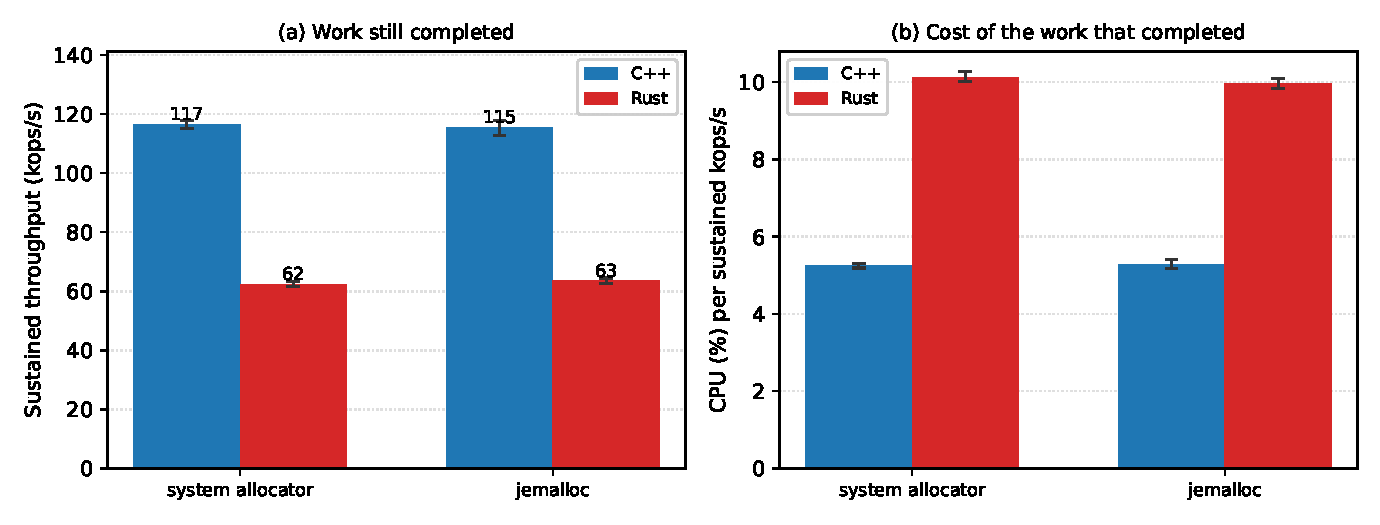
\includegraphics[width=0.78\linewidth]{figures/fig_overload.pdf}
\caption[Phân kỳ qua bão hòa]{Hành vi ở $\OverloadLoad$~kops/s đề nghị, xa quá knee $\SatKnee$~kops/s. Thanh
là median qua \NRepeats{} lần lặp với khoảng bootstrap $95\%$, nhóm sao cho hai
thanh trong nhóm chỉ khác ngôn ngữ. \textbf{(a)} Mỗi variant vẫn hoàn tất:
\OverloadSustainedFaster{} duy trì hệ số $\OverloadThrRatio$ hơn
\OverloadSustainedSlower. \textbf{(b)} Tổng CPU chia cho việc thực sự hoàn tất, điều loại
cách đọc variant giao ít hơn đơn giản làm ít hơn. Nó tiêu
$\OverloadCpuPerOpRatio$ lần CPU mỗi thao tác duy trì, và số CPU
được cộng qua luồng.\label{fig:overload}}
\end{figure}

Effort đi đâu được thu hẹp bằng phép đo chứ không để mở. Qua
bão hòa producer tiêu gần hết thời gian ở hai chỗ ghi trong
Bảng~\ref{tab:idioms}: hàng đợi chặn có giới hạn và tay cầm hoàn tất.
Mục~\ref{sec:contention} cô lập các nguyên thủy đó, và chúng không tái tạo
thứ tự full-service ở mức ý nghĩa. Điều đó loại chúng \emph{riêng lẻ} làm toàn bộ giải thích
cho gap $\OverloadThrRatio\times$. Như Mục~\ref{sec:budget}, không gì trong borrow checker,
kiểm tra bound, hay ownership bị liên quan, và phát hiện không nên trích như
là.

Ba điều lại giới hạn phát hiện cho phép gì. Đó là một thiết kế, dịch vụ shared-nothing với một
yêu cần outstanding mỗi producer và giới hạn hàng đợi $1\,024$, và độ sâu sụp đổ
phụ thuộc cả ba. Đo với harness có producer chặn mỗi yêu cầu, nên nó
mô tả client hình dạng này trải nghiệm chứ không client pipeline.
Và số tuyệt đối thuộc host này. Điều đi theo là thứ tự và nguyên nhân. Dưới
bão hòa lựa chọn ngôn ngữ không quan trọng. Trên nó nguyên thủy đồng bộ thư viện chuẩn
quan trọng, và crossover đủ sắc để so sánh dừng ở tải danh nghĩa
sẽ kết luận ngược.

Crossover cũng liên quan công trình trước gần nhất, báo suy giảm tương đương qua
ngưỡng tốc độ yêu cầu và gán cho runtime async~\cite{arvidsson2025async}. Mục~\ref{sec:rqdiscussion} nói ý nghĩa khi
cùng hình dạng xuất hiện ở đây không có runtime như vậy ở cả hai bên.

\begin{table}[H]
\centering
\small
\caption[Mỗi variant vẫn duy trì gì qua bão hòa]{Mỗi variant vẫn duy trì ở
$\OverloadLoad$~kops/s đề nghị, xa quá knee $\SatKnee$~kops/s: median qua
\NRepeats{} lần lặp trên khoảng tin cậy bootstrap $95\%$. Dưới bão hòa throughput đạt
bị ghim tốc độ đề nghị theo cấu trúc và không thể nói gì về
ngôn ngữ. Ở đây đó là thứ duy nhất có thể. Sử dụng CPU vượt $100\%$ vì được
cộng qua luồng, nên $600\%$ là sáu lõi bận trong mười bốn
ghim.\label{tab:overload}}
\begin{tabular}{@{}l r r@{}}
\hline\hline
Variant & sustained throughput (kops/s) & CPU (\%) \\
\hline
C++ (system alloc) & \mci{146.7}{146.3}{147.2} & \mci{662.8}{662.5}{663.6} \\
C++ (jemalloc) & \mci{146.4}{146.1}{146.9} & \mci{664.3}{663.3}{664.9} \\
Rust (system alloc) & \mci{84.5}{84.2}{84.7} & \mci{681.8}{680.4}{682.5} \\
Rust (jemalloc) & \mci{84.3}{83.9}{84.6} & \mci{680.3}{679.8}{681.5}
\\
\hline
\end{tabular}
\end{table}

\begin{table}[H]
\centering
\small
\caption[Test ghép chính xác qua bão hòa]{Test ghép hoán vị chính xác C++ so với Rust ở
$\OverloadLoad$~kops/s, bộ cấp phát giữ cố định, hiệu chỉnh Holm trên cùng họ
\NTests{} test như Bảng~\ref{tab:significance} chứ không là họ riêng. ``Repeats''
đếm bao nhiêu trong \NRepeats{} hiệu ghép đồng ý dấu median, điều statistic tính từ mean không thể hiện. Không percentile độ trễ được test ở đây, vì
lý do cố định trước Mục~\ref{sec:stats}.\label{tab:overloadtest}}
% The generated metric names are long enough that six l/r columns overrun the text
% block; the first column wraps instead, and the inter-column padding is tightened.
\setlength{\tabcolsep}{4pt}
\begin{tabular}{@{}p{0.24\linewidth} l r c r r@{}}
\hline\hline
Metric & Allocator & Effect (Rust $-$ C++) & Repeats & $p$ & Holm \\
\hline
Sustained throughput (kops/s) & system & \mci{-62.2}{-62.9}{-61.6} & 20/20 & 0.0000019 & 0.000027 \\
Sustained throughput (kops/s) & jemalloc & \mci{-62.2}{-62.7}{-61.6} & 20/20 & 0.0000019 & 0.000027 \\
CPU utilisation (\%) & system & \mci{+19.5}{+17.3}{+19.9} & 20/20 & 0.0000019 & 0.000027 \\
CPU utilisation (\%) & jemalloc & \mci{+16.8}{+15.6}{+17.5} & 20/20 & 0.0000019 & 0.000027
\\
\hline
\end{tabular}
\end{table}

\subsection{Hàng đợi tranh chấp và các primitive hoàn thành (RQ1)}\label{sec:contention}
Kết quả quá tải quy cho khoảng cách hai cấu trúc đồng bộ idiom bắt buộc, nhưng
sự quy kết đó được lập luận từ hình dạng đo toàn dịch vụ. Tiểu mục này
cô lập riêng các cấu trúc đó.

\ContentionProducers{} luồng producer đập vào một hàng đợi có giới hạn dung lượng $1\,024$ trong khi một
consumer duy nhất rút khỏi đó. Mỗi producer gửi một job không làm gì mang tay cầm hoàn thành một lần và chặn
cho đến khi consumer báo hiệu. Không có công việc \texttt{ShardCore} nào chạy trên đường đi. C++ dùng
\texttt{BoundedQueue} viết tay của Mục~\ref{sec:impldetails} với
\texttt{std::promise}/\texttt{std::future}. Rust dùng \texttt{sync\_channel} và một
\texttt{mpsc::channel()} mới mỗi yêu cầu. Mỗi cửa sổ đo kéo dài hai giây sau khởi động nóng.
\ContentionRepeats{} lần lặp xen kẽ được tóm tắt bằng trung vị với khoảng bootstrap và
kiểm định bằng thủ tục hoán vị ghép cặp chính xác của Mục~\ref{sec:stats}.
Bảng~\ref{tab:contention} báo cáo kết quả.

\begin{table}[H]
\centering
\small
\caption[Thông lượng qua các primitive đồng bộ tranh chấp riêng]{Thông lượng qua
hàng đợi có giới hạn và các primitive hoàn thành riêng, với \ContentionProducers{} producer tranh chấp
và dung lượng hàng đợi $1\,024$. Giá trị là trung vị trên \ContentionRepeats{} lần lặp xen kẽ phía trên
khoảng tin cậy bootstrap $95\%$. Kiểm định ghép cặp so C++ với Rust trên thông lượng
bền vững (kops/s). Đo trên máy chủ của Mục~\ref{sec:testbed}.\label{tab:contention}}
\begin{tabular}{@{}l r r r@{}}
\hline\hline
Ngôn ngữ & Thông lượng (kops/s) & Trung bình ns/op & $p$ ghép cặp \\
\hline
C++ & \mci{55.0}{53.7}{58.4} & \mci{18178}{17110}{18632} & \multicolumn{1}{c}{---} \\
Rust & \mci{58.7}{56.8}{61.8} & \mci{17045}{16169}{17594} & 0.226
\\
\hline
\end{tabular}
\end{table}

Các primitive cô lập không tái tạo thứ tự quá tải. C++ duy trì
\ContentionThrCpp{}~kops/s và Rust \ContentionThrRust{}~kops/s, khoảng cách chỉ
$\ContentionRatio\times$ với $p = \ContentionP$. Toàn dịch vụ ở
$\OverloadLoad$~kops/s tách $\OverloadThrRatio\times$, với $p$ đã hiệu chỉnh ở
sàn của họ. Cách đọc trung thực do đó là sự phân kỳ quá tải gồm thêm
công việc mà microbenchmark loại bỏ: \texttt{Request} gắn thẻ lớn hơn phía C++, 
điều phối variant của worker, và các thao tác bản đồ vẫn chạy trong chế độ quá tải.
Điều kết quả vẫn thiết lập hữu ích. Khác biệt bậc độ lớn chỉ ở primitive
bị loại trừ, và tìm cơ chế chuyển sang phần còn lại của đường bàn giao chứ không
sang mô hình an toàn.

\subsection{Sử dụng tài nguyên (RQ3)}\label{sec:resources}
Bảng~\ref{tab:resource} báo cáo sử dụng tài nguyên ở cùng
tải bền vững. Peak resident set size tách bốn biến thể rõ ràng, và tách vậy
dù đọc họ theo cách nào. Khoảng của nó loại trừ không, và hiệu ứng giữ dấu dưới
cả hai bộ cấp phát. Hình~\ref{fig:resources} vẽ cùng phép đo. Panel giữa là
nơi phát hiện của mục này nằm, với hai hiệu ứng bên trong peak RSS vẽ thành
khác biệt ghép cặp trên một trục chung.

Hai hiệu ứng có trong đó, không phải một, và chúng không cùng cỡ. Liên kết
\texttt{jemalloc} tốn $\RssAllocDiffLo$--$\RssAllocDiffHi$~MiB ở cả hai ngôn ngữ. Bản build Rust
tốn thêm $\RssLangDiffLo$--$\RssLangDiffHi$~MiB so với bản build C++ dưới cả hai bộ cấp phát,
với khoảng bootstrap $\RssLangCILo$ đến $\RssLangCIHi$~MiB. Sử dụng tài nguyên theo cả hai, và
hiệu ứng bộ cấp phát lớn hơn một bậc độ lớn. Thứ tự đó phần nào đến từ
kiểm soát công bằng chứ không phải sự thật chung về \texttt{jemalloc}. Cả hai build ghim số arena
giống nhau, để mặc định của không ngôn ngữ nào thành lợi thế tình cờ, và
ghim cao là điều làm metadata arena thành chi phí cố định lớn hai bên. Triển khai
tinh chỉnh \texttt{jemalloc} cho dấu chân thay vì so sánh công bằng sẽ không trả chi phí đó.

Hàng duy nhất trong khối trên của Bảng~\ref{tab:significance} không vượt
hiệu chỉnh là peak RSS dưới
\texttt{jemalloc}, và lý do nằm ở thống kê chứ không phải phần mềm.
Khoảng ở đó chặt, xa không, và $18$ trong $20$ lần lặp ghép cặp đồng ý. Điều đánh bại kiểm định là vài lần chạy báo resident set thấp hơn trung vị biến thể khoảng $30$~MiB
trong khi vẫn không phân biệt được về thông lượng, thời gian tường và số lỗi. Thống kê
hoán vị là trung bình khác biệt ghép cặp, và một lần chạy như vậy chi phối nó. Đây là trường hợp
quy tắc đọc của Mục~\ref{sec:stats} được viết trước để bao phủ, và
Mục~\ref{sec:threats} tiếp nhận cả quy tắc và khuyết điểm đo đằng sau nó.

Sử dụng CPU hành xử khác cả hai, và khác biệt phụ thuộc chế độ chứ không
phải nhiễu. Ở điểm vận hành dưới bão hoà này Rust tiêu thụ CPU \emph{ít} hơn một chút, tối đa
$\CpuDiffAbsMax$ điểm phần trăm, nhất quán dưới cả hai bộ cấp phát và vượt
hiệu chỉnh dưới cả hai. Mục~\ref{sec:overload} thấy dấu đảo qua bão hoà và
biên độ lớn hơn nhiều. Thông lượng đạt được không thêm gì ở đây, vì lý do
Mục~\ref{sec:stats} nêu. Ở điểm dưới bão hoà nó bị ghim vào tải đề nghị, và
chỉ báo cáo để xác nhận điểm được duy trì chứ không chỉ danh nghĩa, và nó vậy trong
$\ReprLoadShortfall\%$.

Hai điều kiện giữ phát hiện bộ nhớ đúng cỡ thực tế. Đó là khác biệt chi phí cố định
chứ không phải chi phí mỗi ngữ cảnh. Ở $5\,000$ UE hoạt động dùng trong quét,
khác biệt bố cục tám byte đo ở Mục~\ref{sec:uecontext} chiếm khoảng
$40$~kB, thiếu hai bậc độ lớn so với khoảng cách. Phần lớn khoảng cách do đó là overhead runtime và
arena bộ cấp phát, không tỷ lệ với khối lượng công việc và sẽ quan trọng tỷ lệ
ít hơn trong triển khai lớn hơn, không phải nhiều hơn. Điều kiện thứ hai là phép đo
thiết lập khác biệt mà không giải thích. Không thu bộ đếm phần cứng hay hồ sơ cấp phát,
nên phần chia giữa dự trữ arena, bộ nhớ đệm mỗi luồng và dấu chân tĩnh
không được giải quyết ở đây. Cả hai điểm được xem lại ở Chương~\ref{chapter:discussion}.

Phát hiện RQ3 do đó không phải ``không phạt tài nguyên'' phẳng mà khoảng chồng lấn
gợi ý, cũng không phải phạt hiệu năng chung. Rust tốn thêm vài megabyte dấu chân cố định, tái lập được và dưới cả hai bộ cấp phát, nhưng nhỏ hơn một bậc độ lớn so với chính lựa chọn
bộ cấp phát. Nó rẻ hơn một chút về CPU khi dịch vụ còn chịu tải, và đắt hơn đáng kể khi không còn.
Trên thao tác trần của Mục~\ref{sec:budget} nó là ngôn ngữ
nhanh hơn trong hai.

\begin{table}[H]
\centering
\small
\caption[Sử dụng tài nguyên ở tải đại diện]{Sử dụng tài nguyên ở tải đề nghị bền vững $\ReprLoad$~kops/s: thông lượng đạt được,
peak RSS và tổng sử dụng CPU. Trung vị trên \NRepeats{} lần lặp phía trên khoảng tin cậy bootstrap
$95\%$. Peak RSS là chỉ số duy nhất ở đây mà khoảng tách bốn
biến thể rõ ràng.\label{tab:resource}}
\begin{tabular}{@{}l r r r@{}}
\hline\hline
Biến thể & thông lượng (kops/s) & peak RSS (MiB) & CPU (\%) \\
\hline
C++ (system alloc) & \mci{27.99}{27.99}{27.99} & \mci{9.4}{9.4}{9.5} & \mci{66.8}{65.8}{68.2} \\
C++ (jemalloc) & \mci{27.95}{27.95}{27.96} & \mci{65.9}{65.9}{65.9} & \mci{64.6}{63.4}{66.1} \\
Rust (system alloc) & \mci{27.99}{27.99}{27.99} & \mci{11.2}{11.1}{11.3} & \mci{63.3}{62.2}{66.0} \\
Rust (jemalloc) & \mci{27.95}{27.92}{27.96} & \mci{67.2}{65.4}{67.3} & \mci{63.0}{62.4}{64.5}
\\
\hline
\end{tabular}
\end{table}

\begin{figure}[ht]
\centering
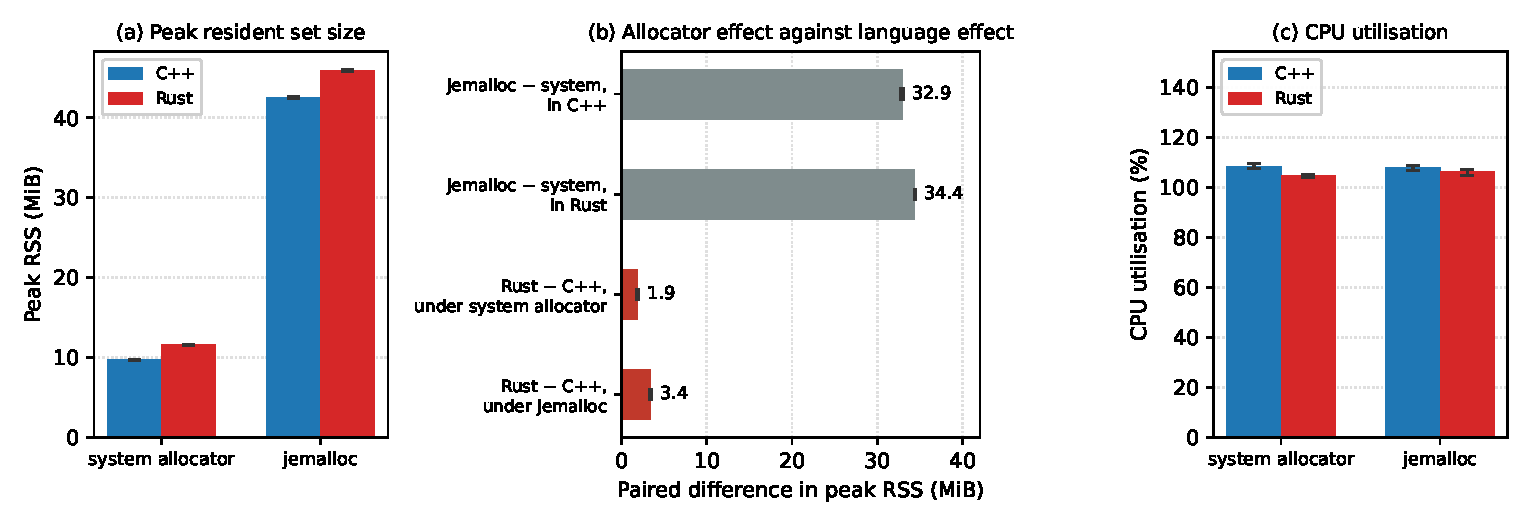
\includegraphics[width=0.78\linewidth]{figures/fig_resources.pdf}
\caption[Sử dụng tài nguyên và hai hiệu ứng trong peak RSS]{Sử dụng tài nguyên ở tải đề nghị bền vững $\ReprLoad$~kops/s, nhóm theo bộ cấp phát để
hai cột trong nhóm chỉ khác ngôn ngữ và hai nhóm chỉ khác bộ cấp phát.
Trung vị trên \NRepeats{} lần lặp với khoảng bootstrap $95\%$. \textbf{(a)} Kích thước resident set đỉnh.
\textbf{(b)} Hai hiệu ứng nó chứa, mỗi cái là khác biệt ghép cặp trên cùng
lần lặp: liên kết \texttt{jemalloc} tốn $\RssAllocDiffLo$--$\RssAllocDiffHi$~MiB, trong khi bản build Rust
tốn thêm $\RssLangDiffLo$--$\RssLangDiffHi$~MiB so với bản C++. Cả hai đều thật, và trên
trục chung hiệu ứng bộ cấp phát lớn hơn một bậc độ lớn. \textbf{(c)} Sử dụng
CPU, cộng qua các luồng, nơi khác biệt chạy chiều ngược và
nhỏ.\label{fig:resources}}
\end{figure}


\chapter{Thảo luận\label{chapter:discussion}}

\section{Tóm tắt phát hiện}
Bảng~\ref{tab:findings} gom phát hiện chính cho mỗi câu hỏi nghiên cứu, cùng
độ mạnh bằng chứng hiện tại. Kết quả an toàn (RQ2) không phụ thuộc môi trường đo
chút nào. Kết quả di chuyển (RQ4) phụ thuộc theo một trục duy nhất, vì thời gian
build là phép đo thời gian, nên được báo dạng tỷ lệ ghép cặp. Kết quả hiệu năng và
tài nguyên phụ thuộc môi trường, và phép chia trung thực giờ nằm trong RQ1 chứ không
giữa các chương. Điểm gối bão hoà, so sánh quá tải, và
so sánh tài nguyên được giải quyết trên máy chủ Mục~\ref{sec:testbed}, và tái lập
qua kiểm soát bộ cấp phát. Đuôi xa dưới bão hoà vẫn chưa giải quyết, vì lý do
thuộc máy chứ không phải phân tích.

\begin{table}[tp]
\centering
\caption[Tóm tắt phát hiện theo câu hỏi nghiên cứu]{Tóm tắt phát hiện theo câu hỏi nghiên cứu và độ mạnh bằng chứng hiện tại.
\label{tab:findings}}
\renewcommand{\arraystretch}{1.25}
\begin{tabular}{@{}p{0.06\linewidth} p{0.62\linewidth} p{0.22\linewidth}@{}}
\hline\hline
RQ & Phát hiện chính & Trạng thái bằng chứng \\
\hline
RQ1 & Câu trả lời chia tại bão hoà. Dưới đó các biến thể đồng ý trong $\PFiftyRange\,\mu$s
($\PFiftySpread\%$) ở trung vị và không có thứ tự đuôi nào phân giải được. Số đầu-cuối chỉ
$\BudgetCoreShareMax\%$ thao tác, nên không thể giới hạn hiệu ứng ngôn ngữ trong mọi trường hợp, trong khi
thao tác đo riêng nhanh hơn $\BudgetCoreRatio\times$ ở \BudgetCoreFaster. Qua
bão hoà chúng phân kỳ dứt khoát: \OverloadSustainedFaster{} duy trì
$\OverloadThrRatio\times$ thông lượng của \OverloadSustainedSlower{} ở
$\OverloadLoad$~kops/s, trong \OverloadThrAgree{} lần lặp dưới cả hai bộ cấp phát. & Quá tải và
thao tác: đã giải quyết. Đuôi xa: chưa giải quyết trên máy này. Cơ chế: đã kiểm. Primitive riêng
không đủ \\
RQ2 & Cả bảy lớp an toàn bộ nhớ và tranh chấp dữ liệu tiêm được ngăn lúc biên dịch trong
Rust an toàn, trong khi ở C++ mỗi lớp biên dịch và chỉ bị bắt, nếu có, lúc runtime và không bộ dò lỗi đơn lẻ
nào. Bảo đảm dừng ở đó: bảy lớp biên biên dịch cả hai ngôn ngữ, và
trên rò rỉ và tràn bản build release công cụ C++ báo điều Rust không. &
Cuối cùng \\
RQ3 & Phạt bộ nhớ tái lập: thêm $\RssLangDiffLo$--$\RssLangDiffHi$~MiB peak RSS trong
bản build Rust dưới \emph{cả hai} bộ cấp phát, nhỏ hơn một bậc độ lớn so với
$\RssAllocDiffLo$--$\RssAllocDiffHi$~MiB của bộ cấp phát. CPU đảo giữa các chế độ: Rust tiêu tối đa
$\CpuDiffAbsMax$ điểm phần trăm ít hơn dưới bão hoà và $\OverloadCpuPerOpRatio\times$ nhiều hơn
mỗi thao tác hoàn thành phía trên. & Bộ nhớ: đã giải quyết, chưa giải thích. CPU: đã giải quyết cả hai
chế độ, dấu đối \\
RQ4 & Đường nối nhỏ và giữ lõi không \texttt{unsafe} lúc biên dịch. Đo so với
cùng thao tác gọi bản địa, không phát hiện chi phí và mọi thuế được giới hạn ở
$\FfiOpBoundPct\%$ một thao tác. Chi phí thật là thiết kế API. Lõi vẫn lộ lúc chạy
với lỗi bộ nhớ ở host C++ chia không gian địa chỉ. Trên các trục áp dụng ngoài
đường nối, $\BuildDepShareCpu\%$ build sạch Rust là mã bên thứ ba và mã riêng dự án biên dịch bằng $\BuildAllFirstPartyCpuRatio$ lần CPU \texttt{g++} cần, thứ tự
dấu chân đảo theo chính sách liên kết, và thành phần so sánh giải quyết $\DepsCore$ crate.
& Cuối cùng. Giây build tuyệt đối gắn host, tỷ lệ thì không \\
\hline
\end{tabular}
\end{table}

\section{Thảo luận về các câu hỏi nghiên cứu}\label{sec:rqdiscussion}
\paragraph{RQ1 (độ dự đoán được).} RQ1 có hai nửa, dưới bão hoà và qua nó, và
chiến dịch trả lời chúng đủ khác để báo cáo một mình sẽ bóp méo
kết quả.

Dưới bão hoà hai ngôn ngữ tương đương về hành vi trung tâm, với biên độ không triển khai
nào để ý. Khác biệt ghép cặp nhỏ ở trung vị vượt hiệu chỉnh là
một phần nhỏ của thao tác $80\,\mu$s. Đuôi xa trong chế độ này là chuyện khác, và triển khai
cũng quan tâm. Ở đó kết quả là null mà máy này không thể biến thành
thứ tự, nên tương đương tuyên bố ở đây không chạm tới nó. Kết quả trung tâm nhất quán với
bằng chứng rộng hơn rằng
kiểm tra an toàn của Rust phần lớn được CPU out-of-order hiện đại
hấp thụ~\cite{balasubramanian2017rust,emmerich2019drivers}. Nó cũng yếu hơn
trông, vì lý do Mục~\ref{sec:budget} nêu. Thao tác hai ngôn ngữ
thực thi là $\BudgetCoreShareMax\%$ những gì quét đo. Null đầu-cuối trong
thiết kế chi phối bởi đánh thức giữa luồng do đó nói về thiết kế chứ không
về ngôn ngữ. Đo riêng, thao tác khác $\BudgetCoreRatio\times$.

Qua bão hoà câu trả lời đổi loại, và đây là kết quả duy nhất trong nghiên cứu trả lời
RQ1 đúng theo nghĩa RQ1. Bản build C++ duy trì $\OverloadThrRatio$ lần thông lượng của
bản Rust trong khi tiêu nhiều CPU hơn mỗi thao tác hoàn thành, tái lập được và ở sàn
đã hiệu chỉnh của cả họ kiểm định (Mục~\ref{sec:overload}). Vậy dạng thực tế câu trả lời RQ1
không phải lựa chọn ngôn ngữ vô quan với độ dự đoán. Nó vô quan \emph{cho đến khi
dịch vụ không còn chịu tải}, và lúc đó nó quyết định bao nhiêu
công việc vẫn được làm. So sánh dừng ở tải danh nghĩa, như hầu hết trong tài liệu
này, sẽ kết luận ngược với cùng bộ máy.

Điều đó đặt lại công trình tiền nhiệm gần nhất thay vì chỉ đồng ý. Arvidsson và Kaller
đo đại lượng này cho thủ tục mặt điều khiển 5G và thấy phần trăm thứ 99 của Rust suy giảm
nhanh hơn qua ngưỡng tốc độ yêu cầu. Họ truy về
\texttt{async}/\texttt{await} không stack, cho phép chuyển ngữ cảnh ngay trước khi thao tác I/O
bắt đầu~\cite{arvidsson2025async}. Mục~\ref{sec:relatedwork} chấp nhận sự quy kết đó, và
nghiên cứu này được xây để loại nhiễu đằng sau: một worker mỗi shard qua hàng đợi chặn có giới hạn,
và không runtime bất đồng bộ hai bên.

Mục~\ref{sec:rqs}
cam kết trước mỗi kết quả sẽ có nghĩa gì, và nhánh thứ hai là nhánh
kích hoạt. Suy giảm qua ngưỡng tốc độ xuất hiện với mô hình đồng thời giữ cố định, nên
runtime bất đồng bộ không thể là nơi duy nhất hiệu ứng như vậy bắt đầu. Dự đoán cũng
đặt tên nơi nhìn trước nếu điều đó xảy ra: kiểm tra biên và tràn
~\cite{zhang2022runtime,harris2023morello}. Phần đó sai. Hiệu ứng
chỉ xuất hiện khi đường bàn giao tranh chấp, trỏ thay vào hai primitive chặn của
hai thư viện chuẩn ghi trong Bảng~\ref{tab:idioms}. Mục~\ref{sec:contention}
rồi kiểm tra liệu các primitive đó riêng giải thích khoảng cách, và chúng không tái tạo
thứ tự toàn dịch vụ ở mức ý nghĩa. Điều đó thu hẹp nguyên nhân vào công việc thêm trên đường bàn giao C++
chứ không phải mô hình an toàn. Ghi rằng dự đoán giải quyết ngược giả thuyết đầu
của chính nó, và microbenchmark theo sau tinh chỉnh quy kết thay vì xác nhận,
hữu ích hơn cho nghiên cứu sau hơn là lặng thay bằng lời giải thích còn sống.

\paragraph{RQ2 (an toàn).} Kết quả không phụ thuộc môi trường. Điều làm nó
thú vị không phải nửa xác nhận kỳ vọng, mà nửa giới hạn nó. Trong
phạm vi bảo đảm tuyệt đối theo một nghĩa cụ thể, và khác biệt với C++ là khác
loại chứ không phải mức độ. Trình biên dịch từ chối build loại trừ lỗi khỏi
mọi thực thi. Bộ dò lỗi chỉ loại trừ khỏi thực thi bài kiểm thử có công cụ
tình cờ đi qua. Điều tuyệt đối là độ phủ thực thi, không phải độ rộng danh mục.
Phạm vi vẫn là $\FaultClasses$ chương trình viết cho nó.
Điều đó khớp bằng chứng CVE rằng lỗi an toàn bộ nhớ Rust luôn liên quan
\texttt{unsafe}~\cite{xu2021rustcve}, và cảnh báo unsafety vẫn lan
qua phụ thuộc~\cite{evans2020rust}, đó là lý do giữ lõi không \texttt{unsafe}
quan trọng. Seam double-free là bằng chứng đó tái tạo trong điều kiện kiểm soát: lớp
duy nhất trong danh mục mà Rust an toàn từ chối và Rust unsafe không.

Ca duy nhất vượt chương trình đã viết là lỗi vòng đời của
Mục~\ref{sec:safetyresults}. Nó được tìm trong hiện thực, không viết cho
danh mục, và sửa bức tranh hai hướng. Nó củng cố lập luận
chi phí. Một lỗi thật trong mã viết để đúng sống sót toàn bộ bộ xác minh
của nghiên cứu này, tức kiểm thử, vector tương đương và ba bộ dò lỗi, chỉ vì
không gì đi qua đường đó. Phát hiện runtime phụ thuộc độ phủ kiểm thử là đề xuất
yếu hơn trong thực tế so với trong bảng mà mỗi hàng được lái có chủ đích.

Nó cũng
thu hẹp điều có thể ghi cho Rust, vì đóng góp ngôn ngữ ở đó là bounds
check chứ không phải chứng minh. Rust an toàn biến undefined behaviour thành panic xác định, đó là
tuyên bố khác và kém hơn ngăn lỗi. Tổng quát hoá trung thực là
bảo đảm đáng ngân sách là \emph{kiểm tra mặc định} chứ không phải \emph{loại trừ lúc
biên dịch}. Nguyên nhân gốc đáng đặt tên, vì đó là rủi ro của phương pháp
chứ không phải ngôn ngữ nào. Đặc tả nêu lệnh cấm mà không gán
cơ chế để mỗi hiện thực lỗi theo idiom riêng. Hai idiom ở đây là
panic và use-after-free.

Nơi bảo đảm dừng quan trọng không kém cho nhà cung cấp quyết định Rust mua gì, và hai
lớp biên minh hoạ vì lý do khác nhau. Deadlock thứ tự khóa cho thấy Rust
suy luận về \emph{aliasing} chứ không về \emph{thứ tự acquisition}. Guard \texttt{Mutex} là
giá trị thường mà borrow checker theo dõi vòng đời hoàn hảo, và theo dõi hoàn hảo
không nói hai luồng lấy khóa theo thứ tự tương thích. Công cụ quanh ngôn ngữ xác nhận đây là biên chứ không phải artefact ví dụ tiêm.
Phát hiện deadlock tĩnh cho Rust là bài toán nghiên cứu đang hoạt động
riêng~\cite{zhang2026deadlock}, và bộ kiểm tra mô hình cho mã kernel Rust được thúc đẩy
rõ ràng bởi quan sát ownership và borrowing để lại tranh chấp dữ liệu, deadlock và
livelock vẫn chạm tới~\cite{tang2025converos}.

Lost update sắc hơn nữa. Nó thoát
ThreadSanitizer đúng lý do thoát borrow checker, như
Mục~\ref{sec:safetyresults} nêu. Với mọi truy cập đồng bộ đúng không có
truy cập không đồng bộ để tìm. Cũng không lớp lề. Trong nghiên cứu thực địa $105$
lỗi đồng thời thật, khoảng một phần ba ca không deadlock vi phạm thứ tự lập trình viên
định, không phải khóa của họ, và tác giả ghi ý định như vậy không diễn đạt
dễ qua khóa~\cite{lu2008mistakes}. Phân biệt
nó bộc lộ, giữa race dữ liệu và điều kiện đua, là điều cụm ``an toàn luồng'' thường gộp, và Rust chỉ loại bỏ
cái đầu.

Hệ quả thực hành là áp dụng Rust loại bỏ hoàn toàn một loại lỗi đồng thời
trong khi để nguyên loại kia. Loại còn lại là loại thất bại
im lặng, làm hỏng bộ đếm hay quyết định trạng thái thay vì crash. Kế hoạch di chuyển
coi ``an toàn bộ nhớ'' là ``an toàn đồng thời'' sẽ do đó lập ngân sách review và kiểm thử
sai. Đó là lý do biên được báo cáo như kết quả hạng nhất chứ không phải điều kiện.
Hình~\ref{fig:boundary} vẽ chính biên, với hai nửa
bảo đảm hai bên đường và cơ chế thực thi, hoặc vắng mặt
của nó, được đặt tên mỗi panel. Nó mang hai ca đồng thời thay vì cả bảy ngoài
bảo đảm, vì chúng là cặp làm rõ phân biệt, và
Bảng~\ref{tab:taxonomy} giữ toàn danh mục.

\begin{figure}[ht]
\centering
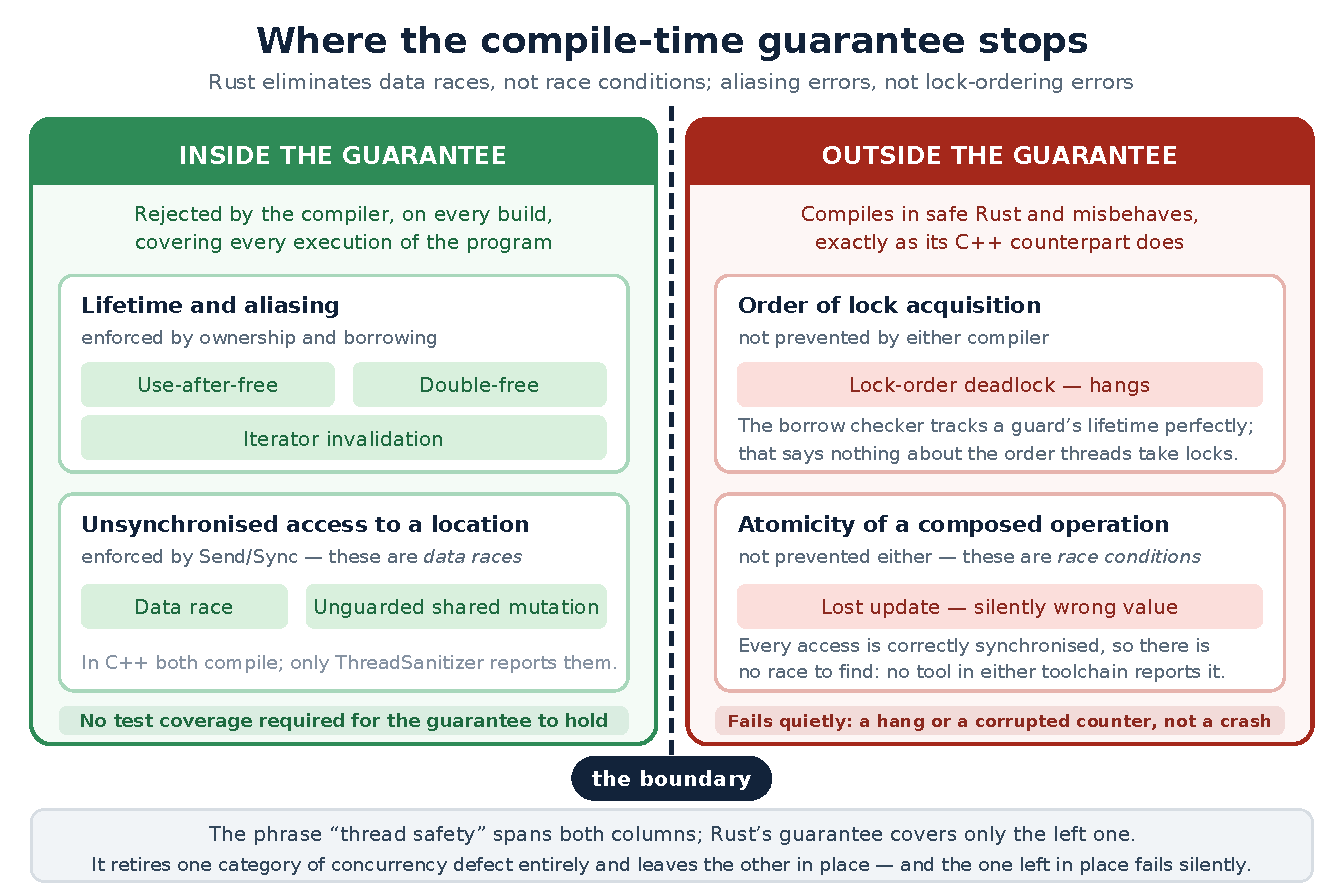
\includegraphics[width=0.78\linewidth]{diagrams/pdf/17_guarantee_boundary.pdf}
\caption[Nơi bảo đảm biên dịch của Rust dừng]{Nơi bảo đảm biên dịch dừng. Bên trái là các lớp Rust an toàn từ chối
hẳn, nhóm theo \emph{cơ chế} từ chối thay vì theo họ
lỗi: ownership và borrowing cho lỗi vòng đời và aliasing,
đó là lý do vô hiệu hoá iterator nằm cùng chúng, và kỷ luật \texttt{Send}/\texttt{Sync}
cho truy cập không đồng bộ vào một vị trí. Bên phải là các lớp danh mục đưa vào để tìm cạnh, mà không trình biên dịch nào ngăn. Sơ đồ đặt tên một
lớp mỗi cơ chế và không phải danh mục, mà
Bảng~\ref{tab:defectmap} liệt kê đầy đủ: use-after-move thuộc
các ca ownership bên trái và handle không an toàn luồng chia sẻ với \texttt{Send}/\texttt{Sync}
bên đó, trong khi rò rỉ, tràn bản build release, lỗi worker, seam double-free
và forgotten guard nằm cạnh hai ca bên phải. Cụm ``an toàn luồng'' trải
cả hai bên đường, và bảo đảm chỉ bao trái. Đường lại di chuyển thêm một lần
nữa so với sơ đồ thể hiện, vì chương trình viết \texttt{unsafe} vượt qua nó
tự nguyện.\label{fig:boundary}}
\end{figure}


\chapter{Kết luận và Công việc tương lai\label{chapter:conclusions}}

Luận văn này so sánh C++ hiện đại và Rust trên một dịch vụ Quản lý Ngữ cảnh UE mô hình hoá theo
một thành phần gNB-CU-CP thực của Nokia, theo bốn chiều: độ dự đoán được của độ trễ đuôi, ngăn
chặn lỗi tại thời điểm biên dịch, chi phí mô hình an toàn, và chi phí áp dụng tăng dần. Xây dựng
trên một đặc tả cố định duy nhất và chạy qua cùng các đường mã, hai bản hiện thực cho phép tách
hiệu ứng ngôn ngữ khỏi khác biệt về thiết kế và kỹ năng.

Ba kết luận theo sau từ bằng chứng. Thứ nhất, về an toàn, khác biệt là khác biệt về \emph{loại}, và
nó có một cạnh xác định. Rust an toàn từ chối cả bảy lớp lỗi an toàn bộ nhớ và tranh chấp dữ liệu
được tiêm vào tại thời điểm biên dịch, và một trong bảy lớp đó là lớp mà không bộ dò lỗi C++ nào
báo cáo. Các mối nguy mà C++ chỉ có thể hy vọng bắt được trong một bài kiểm thử có gắn công cụ trở
thành không thể viết. Cạnh đó dừng ở đó.
Cả bảy lớp biên
đều biên dịch và hành xử sai trong Rust an toàn đúng như trong C++, và trên hai lớp trong số đó
công cụ C++ là bên báo cáo. Vì vậy bảo đảm được mô tả chính xác nhất như sau. Rust loại bỏ tranh
chấp dữ liệu, không phải điều kiện đua, và lỗi aliasing, không phải lỗi thứ tự khóa, rò rỉ, số học
quấn vòng hay ngăn chứa lỗi, và nó không loại bỏ lớp nào trong số đó ở vùng được đánh dấu
\texttt{unsafe}. Ở nơi các lỗi biên được bắt, chúng được
bắt tại thời điểm kiểm thử, trong hai trong ba trường hợp chỉ sau khi được viết lại theo các
primitive của bộ kiểm tra mô hình, đó là một chi phí thực và khác với chi phí của bộ dò lỗi.

Thứ hai, về di chuyển
chi phí chủ yếu do thiết kế API và đường cong học tập, không phải bởi bất kỳ thuế thời gian chạy
nào. Một lõi Rust không sửa đổi có thể được điều khiển từ C++ qua một đường nối mỏng, cô lập
\texttt{unsafe}, có chi phí trên một thao tác thực, đo so với cùng thao tác gọi bản địa, được giới
hạn ở $\FfiOpBoundPct\%$. Các chi phí mà kỹ sư build thường nêu trước không đổi thứ tự đó.
Phần lớn chi phí build thêm của Rust là biên dịch phụ thuộc chứ không phải công việc của chính
trình biên dịch, khoảng cách kích thước nhị phân là chính sách liên kết và đảo chiều khi chính sách
được khớp, và thành phần được so sánh không giải quyết mã bên thứ ba nào. Nơi C++ dẫn trước là vòng
lặp sửa-biên dịch, và nó chỉ dẫn trước với các sửa đổi nằm trong một đơn vị dịch.

Thứ ba, về hiệu năng bằng chứng chia đôi hai lần trước khi chia theo tài nguyên. Nó chia trước
theo \emph{cái gì đang được đo}, rồi theo \emph{liệu dịch vụ còn chịu tải được}. Làm đúng cả hai
phép chia là chỉnh sửa quan trọng nhất của nghiên cứu đối với chính nó, và mỗi phép được phát hiện
chứ không phải dự đoán trước. Một thao tác đầu-cuối trong thiết kế này là $\BudgetCoreShareMax\%$
công việc ngôn ngữ thực hiện, phần còn lại là bàn giao giữa luồng mà hệ điều hành thực hiện, nên
một kết quả null đầu-cuối không thể giới hạn hiệu ứng ngôn ngữ. Đo riêng thao tác thì hai ngôn ngữ
không tương đương. Rust nhanh hơn, theo $\BudgetCoreRatio\times$, vì
lựa chọn bố cục bảng băm của thư viện chuẩn chứ không vì điều gì
liên quan đến an toàn.

Phép chia thứ hai là theo chế độ, và nó quan trọng hơn. Dưới bão hoà hai ngôn ngữ tương đương ở
trung vị cho mọi mục đích triển khai quan tâm, và đó là kết quả thực về các triển khai dạng này.
Tương đương là thực tiễn chứ không phải thống kê, vì kiểm định ghép cặp vẫn phân giải
$\PFiftyDiffAbsMax\,\mu$s nghiêng về Rust dưới cả hai bộ cấp phát. Đuôi xa của chúng vẫn không phân
giải được trên máy ảo hoá, đó là thừa nhận về dụng cụ đo. Qua bão hoà chúng không tương đương. Bản
build C++ duy trì $\OverloadThrRatio\times$ thông lượng của bản build Rust, trong
\OverloadThrAgree{} lần lặp xen kẽ dưới cả hai bộ cấp phát, trong khi tiêu thụ
$\OverloadCpuPerOpRatio\times$ CPU trên mỗi thao tác hoàn thành, và các primitive cô lập không tái
tạo thứ tự đó ở mức ý nghĩa (Mục~\ref{sec:contention}). Về bộ nhớ bản build Rust mang thêm vài MiB
dấu chân cố định dưới cả hai bộ cấp phát, nhỏ hơn một bậc độ lớn so với chi phí của chính lựa chọn
bộ cấp phát.

Gộp lại, chúng ủng hộ một tuyên bố hẹp, hẹp hơn tuyên bố luận văn này dự kiến
đưa ra. Đối với các dịch vụ mặt điều khiển có trạng thái, đồng thời, có thể phân vùng dạng này, và
\emph{ở tải danh nghĩa}, lựa chọn giữa C++ hiện đại và Rust không phải quyết định hiệu năng. Đó là
quyết định về lớp lỗi nào tổ chức muốn làm không thể viết, và liệu tổ chức có trả chi phí kỹ thuật
và học tập để đạt được hay không. Dưới quá tải nó lại thành quyết định hiệu năng, và hiện nay ủng
hộ C++. Lý do nằm ở hạ tầng đồng thời chứ không phải bảo đảm của ngôn ngữ nào, và dịch vụ bắt buộc
phải suy giảm êm không thể coi chúng là phụ. Điều luận văn này bổ sung do đó là một dụng cụ đo chứ
không phải phán quyết: một đặc tả cố định, một cặp hiện thực đã kiểm thử tương đương, một khung đo
có thể tái lập vượt qua điểm gối bão hoà, một phân rã nói phần nào trong số đo đó ngôn ngữ phải
chịu trách nhiệm, và một danh mục lỗi ánh xạ cả phần bảo đảm bao phủ lẫn nơi nó dừng.

Một số hướng mở rộng công việc, mỗi hướng là biện pháp trực tiếp cho một hạn chế đã nêu ở trên.
Ưu tiên tức thời là chiến dịch bare-metal, mục tiêu giờ đã hẹp: điểm gối bão hoà và so sánh quá
tải đã được giải quyết, nên bare-metal sẽ mang lại đuôi xa dưới bão hoà. Bộ đếm phần cứng và hồ sơ
cấp phát thuộc cùng chuyến đo và là khoảng trống dụng cụ đo rõ nhất trong nghiên cứu. Chúng sẽ biến
kết quả bộ nhớ của Mục~\ref{sec:resources} từ quan sát thành giải thích, và xác nhận hoặc bác bỏ
lời giải thích về cục bộ bộ nhớ đệm mà Mục~\ref{sec:budget} đưa ra cho khoảng cách ở mức thao tác.
Ngoài ra:

\begin{itemize}
\item Phát lại các trace sản xuất đã ẩn danh hoá thay cho khối lượng công việc tổng hợp, để hỗn hợp
  thao tác được xác thực chứ không chỉ được biện minh bằng đặc tả.
\item Mở rộng so sánh sang thêm các phân hệ mặt điều khiển, hoặc sang đường L2/PHY nặng dữ liệu, nơi
  trạng thái dùng chung có thể thay đổi và áp lực cấp phát sẽ kiểm tra hai ngôn ngữ khác với thiết
  kế không chia sẻ.
\item Mở rộng danh mục lỗi dọc theo biên được ánh xạ ở đây. Lạm dụng \texttt{unsafe}, và
  các lớp biên dưới bộ kiểm tra mô hình toàn chương trình thay vì mô hình thu nhỏ thủ công, là các
  bước tiếp theo hiển nhiên. Một bộ kiểm tra bao phủ chương trình Rust cùng phụ thuộc nước ngoài
  của nó~\cite{pearce2026rustmc} sẽ chạm đường nối của
  Mục~\ref{sec:migrationresults}, mà nghiên cứu này đo chi phí nhưng không khám phá các xen kẽ của
  nó.
\item Đánh giá runtime async của Rust so với mô hình một luồng mỗi shard dùng ở đây, dưới các kiểm
  soát nghiên cứu này áp đặt. Điều đó sẽ tách sự phân kỳ đuôi mà Arvidsson và Kaller quy cho
  \texttt{async}/\texttt{await} không stack~\cite{arvidsson2025async} khỏi bản thân ngôn ngữ,
  và sẽ xác định bao nhiêu phần khoảng cách Olsson và Stenstr\"om đo giữa
  Rust bất đồng bộ và DPDK~\cite{olsson2023asyncpackets} thuộc runtime chứ không phải framework.
\item Đo chi phí cô lập trong tiến trình hai heap tại đường nối, vì lõi không \texttt{unsafe} cần
  được bảo vệ cũng như
  được xác minh~\cite{rivera2021galeed,kirth2022pkrusafe}.
\item Theo dõi mật độ lỗi và công sức review khi Rust được áp dụng tăng dần trong mã nguồn RAN sản
  xuất.
\end{itemize}


\cleardoublepage
\phantomsection
\addcontentsline{toc}{chapter}{\bibname}
\printbibliography

\backmatter
\begin{appendices}

% Inside the appendices, \appendix takes the title where \chapter would.
\appendix{Viết tắt và thuật ngữ chính\label{appendix:terms}}
Các viết tắt và thuật ngữ dùng xuyên suốt luận văn, cho độc giả ngoài lĩnh vực viễn thông.

\begin{table}[H]
\centering
\caption[Viết tắt và thuật ngữ chính]{Viết tắt và thuật ngữ chính dùng xuyên suốt luận văn.\label{tab:abbrev}}
% One size down so that a glossary of this length shares a page with the appendix
% heading inside the class's 23cm text block. The \singlespacing is redundant while
% the body is single-spaced, and is kept so the table survives a change back.
\singlespacing
\footnotesize
\renewcommand{\arraystretch}{1.2}
\begin{tabular}{@{}p{0.21\linewidth} p{0.71\linewidth}@{}}
\hline\hline
Thuật ngữ & Ý nghĩa \\
\hline
RAN & Mạng truy nhập vô tuyến: phần mạng di động nối thiết bị với lõi \\
NG-RAN & RAN thế hệ tiếp theo, kiến trúc mạng truy nhập vô tuyến 5G \\
IMT-2030 & Khung ITU cho thế hệ sau 5G, thường gọi là 6G \\
AI-RAN & Kiến trúc trong đó AI và khối lượng RAN chia sẻ một hạ tầng tăng tốc \\
gNB & Trạm gốc 5G (``next-generation NodeB'') \\
gNB-CU / DU & Đơn vị trung tâm / Đơn vị phân tán: hai nửa tách rời của gNB \\
gNB-CU-CP & Phần mặt điều khiển của đơn vị trung tâm: lớp hệ thống được nghiên cứu ở đây \\
UE & Thiết bị người dùng: thiết bị đầu cuối (điện thoại, modem) gắn vào mạng \\
UECM & Quản lý ngữ cảnh UE: phân hệ quản lý trạng thái theo UE được hiện thực lại ở đây \\
RRC & Điều khiển tài nguyên vô tuyến: giao thức báo hiệu mặt điều khiển giữa UE và gNB \\
DRB & Kênh mang dữ liệu vô tuyến theo UE: kênh dữ liệu mặt người dùng thiết lập trong phiên \\
Mặt điều khiển & Đường báo hiệu và quản lý, trái với đường dữ liệu mặt người dùng \\
Độ trễ đuôi & Độ trễ phần trăm cao (p99, p99.9), chỉ số thời gian hướng trường hợp xấu nhất \\
Jitter & Mức độ độ trễ dao động giữa các thao tác, trái với giá trị điển hình \\
Bão hoà & Tải đề nghị vượt quá khả năng dịch vụ theo kịp và yêu cầu bắt đầu xếp hàng \\
Shard & Một trong các lát trạng thái UE độc lập, mỗi lát thuộc đúng một luồng worker \\
FFI & Giao diện hàm nước ngoài: gọi Rust từ C++ qua ABI C \\
HDR histogram & Biểu đồ tần suất dải động cao, dùng để ghi độ trễ chính xác \\
\hline
\end{tabular}
\end{table}

\appendix{Giao thức tìm kiếm tài liệu\label{appendix:search}}
Mục~\ref{sec:approach} báo cáo hai phát hiện mà tìm kiếm này tạo ra. Giao thức được ghi ở đây để
khoảng trống mà nghiên cứu tuyên bố có thể được kiểm tra chứ không phải tin theo lời nói.

Tài liệu ứng viên được thu thập từ ACM Digital Library, IEEE Xplore, USENIX và Google
Scholar, dùng các tổ hợp thuật ngữ \emph{Rust}, \emph{C++}, \emph{memory safety}, \emph{tail
latency}, \emph{systems programming}, \emph{performance comparison}, và \emph{RAN} / \emph{5G
control plane}. Tìm kiếm giới hạn ở hội nghị có phản biện, trừ khi báo cáo ngành hoặc
chính phủ chính là đối tượng nghiên cứu, như các quy định an toàn bộ nhớ và thống kê lỗ hổng của
nhà cung cấp.
Tập kết quả sau đó được mở rộng bằng truy vết trích dẫn ngược và xuôi từ các bài an toàn Rust
cốt lõi, và lọc giữ công trình hoặc đo ngôn ngữ hệ thống bằng thực nghiệm, hoặc hình thức hoá bảo
đảm của Rust, hoặc báo cáo kinh nghiệm áp dụng. Tài liệu miền (đặc tả 3GPP và
khảo sát O-RAN) được thêm riêng để cố định bối cảnh kiến trúc.

Chỉ các nguồn trên sẽ bỏ sót công trình tiền nhiệm gần nhất, đó là lý do hai nguồn nữa được thêm.
Các luận văn do nhà cung cấp lưu trữ gần nghiên cứu này nhất (Mục~\ref{sec:relatedwork}) không
xuất hiện trong cơ sở dữ liệu trích dẫn nào: không có trong Crossref, OpenAlex, DBLP hay Semantic
Scholar. Truy vết xuôi hay ngược không chạm tới chúng, vì không có mục được lập chỉ mục trích dẫn
chúng và danh sách tài liệu tham khảo của chúng không được nộp. Chúng được tìm bằng cách tìm trực
tiếp trên kho lưu trữ thể chế, DiVA cho các trường Bắc Âu và Finna cho các trường Phần Lan. Cùng hai
tìm kiếm đó thiết lập sự vắng mặt ở phía kia. Finna, liên kết các kho luận văn đại học Phần Lan,
không trả luận văn nào về Rust trong bối cảnh truy nhập vô tuyến hay viễn thông. Tìm theo tác giả
thuộc Nokia trong các ấn phẩm được lập chỉ mục trên OpenAlex cũng không trả kết quả. Các thực thể của
hãng giữ khoảng ba vạn công trình được lập chỉ mục, vài trăm trong số đó về mạng truy nhập vô tuyến,
và một công trình nhắc Rust, trong một bản thảo trước in không liên quan về giám sát thực thi tin
cậy.

Một ghi chú thực tiễn thuộc cùng giao thức, vì nó làm méo tìm kiếm ngây thơ. Truy vấn văn bản tự do
cho \emph{Rust} trong các chỉ mục chung xếp bệnh học thực vật và hóa học ăn mòn trên ngôn ngữ lập
trình, nên cần truy vấn giới hạn trường hoặc lĩnh vực.

\appendix{Thiết kế thống kê: thành viên họ và khả năng phân giải\label{appendix:stats}}
Mục~\ref{sec:stats} cố định so sánh nào vào họ đã hiệu chỉnh và thiết kế nhìn sâu bao xa vào một
khác biệt. Ba điểm đằng sau các cam kết đó được ghi ở đây thay vì trong văn bản chính.

\paragraph{Vì sao một so sánh không phân giải được không miễn phí.}
Kiểm thử thông lượng đạt được dưới bão hoà sẽ đo lại điểm vận hành chứ không phải mã. Nó cũng tốn
các so sánh có thể phân giải điều gì, vì Holm chia ngân sách trên cả họ và một kiểm định không tách
gì vẫn chiếm một phần. Qua bão hoà lập luận tương tự chạy ngược. Điều mỗi biến thể vẫn duy trì ở đó
không bị ghim vào gì, nên loại trừ nó sẽ bỏ đi đại lượng quan sát duy nhất chế độ đó cung cấp.

\paragraph{Vì sao không có phần trăm nào được kiểm định khi quá tải.}
Dưới lịch gửi cố định dự định, một producer không theo kịp sẽ tụt lại tích luỹ, nên phần trăm đo ở
đó báo cáo tồn đọng tích luỹ trước cửa sổ cắt nó. Gắn giá trị $p$ vào cận dưới sẽ kiểm định bộ
điều khiển chứ không phải phần mềm.

\paragraph{Các sàn mà thiết kế có thể chạm.}
Một kiểm định chính xác trên $n$ cặp không thể trả $p$ hai phía dưới $2/2^{n}$, và sau hiệu chỉnh một
họ $m$ so sánh giá trị điều chỉnh nhỏ nhất có thể là $m$ lần số đó. Đó là nguồn gốc của
$\MinAttainableP$ và $\CorrectedFloor$ ở Mục~\ref{sec:stats}. Một chiến dịch có sàn đã hiệu chỉnh
nằm trên ngưỡng đang áp dụng không thể chứng minh ý nghĩa dù hiệu ứng lớn đến đâu, nên báo ``không
có ý nghĩa'' từ chiến dịch như vậy sẽ nói nhiều về số lần lặp hơn về ngôn ngữ.

\appendix{Cấu hình máy chủ và chiến dịch\label{appendix:config}}
Bảng~\ref{tab:testbed} liệt kê máy đo của Mục~\ref{sec:testbed} so với giao thức bare-metal mà số
đuôi cấp testbed yêu cầu. Bảng~\ref{tab:params} gom cấu hình dịch vụ, khối lượng công việc và
chiến dịch, các giá trị suy ra của chúng Mục~\ref{sec:workload} trích dẫn.

\begin{table}[H]
\centering
\small
\caption[Máy chủ đã dùng và giao thức testbed còn phải thực hiện]{Máy chủ mà kết quả được báo cáo đo trên, so với giao thức mà số đuôi cấp testbed yêu
cầu (\texttt{bench/TESTBED.md}). Các hàng hai cột trùng là thuộc tính của mã nguồn và
trình biên dịch. Các hàng khác nhau là điều một chiến dịch bare-metal vẫn mang lại. Chỉ khác biệt
cuối giờ còn tốn một kết quả, vì điểm gối bão hoà và so sánh tài nguyên đã được giải quyết trên máy
này: phần còn lại là đuôi xa dưới bão hoà.\label{tab:testbed}}
\renewcommand{\arraystretch}{1.2}
\begin{tabular}{@{}R{0.22\linewidth} R{0.35\linewidth} R{0.35\linewidth}@{}}
\hline\hline
Khía cạnh & Dùng cho kết quả báo cáo ở đây & Yêu cầu cho số đuôi cấp testbed \\
\hline
Máy chủ & Máy chủ hai socket chuyên dụng, $2\times$ Xeon E5-2680~v4, $16$ vCPU, một nút NUMA & Cùng lớp máy, không hypervisor \\
Ảo hoá & Khách KVM: tần số và turbo do host điều khiển và không quan sát được & Không. Governor và turbo đặt và xác minh \\
CPU steal & Khác không, cỡ $10$~ms thời gian vCPU mỗi giây & Không \\
Kernel & Rocky Linux~8.10, kernel bản phân phối & Giống, với \texttt{isolcpus} và \texttt{nohz\_full} trên lõi benchmark \\
Toolchain & \texttt{g++~15.1.1}, \texttt{rustc~1.97} & \texttt{g++~15.1.1}, \texttt{rustc~1.97} \\
Ghim CPU & Lõi $2$--$15$ qua \texttt{taskset}, $7$ shard, $7$ producer & Giống, trên lõi cũng bị gỡ khỏi bộ lập lịch \\
Đa luồng đồng thời & Vắng trong topology khách thấy. vCPU có chia anh em luồng hay không do host quyết & Vắng hoặc tắt, và xác minh trên máy \\
Khởi động nóng & Phần đầu mỗi lần chạy bỏ & Phần đầu mỗi lần chạy bỏ \\
Lần lặp và xen kẽ & \NRepeats{} lần lặp, bốn biến thể xen kẽ mỗi lần & \NRepeats{} lần lặp, bốn biến thể xen kẽ mỗi lần \\
Ghi môi trường & \texttt{bench/capture\_env.sh}, lưu cùng mỗi kết quả & \texttt{bench/capture\_env.sh}, lưu cùng mỗi kết quả \\
Bộ đếm phần cứng & Không có trong khách & Có: khoảng trống dụng cụ đo rõ nhất \\
\hline
Đủ cho & Tương đương, tiêm lỗi, cấu trúc FFI, điểm gối bão hoà và so sánh quá tải, và so sánh tài nguyên & Thêm đuôi xa dưới bão hoà, và cơ chế đằng sau kết quả tài nguyên và thao tác \\
\hline
\end{tabular}
\end{table}

\begin{table}[H]
\centering
\small
\caption[Cấu hình dịch vụ, khối lượng công việc và chiến dịch]{Cấu hình dịch vụ được kiểm thử, khối lượng công việc điều khiển nó, và chiến dịch
đo. Tham số dịch vụ cố định bởi đặc tả đóng băng, một ngoại lệ: số shard đặt khớp lõi máy cung cấp
(Mục~\ref{sec:testbed}). Tất cả, kể cả ngoại lệ đó, giống nhau ở hai ngôn ngữ. Số chiến dịch sinh từ
nhật ký đo cùng các
bảng báo cáo chúng. Tải đại diện không chọn bằng mắt mà suy ra, là tải quét bận nhất mà cả bốn biến
thể build vẫn giữ p99 dưới $5$~ms.\label{tab:params}}
\footnotesize
\renewcommand{\arraystretch}{1.05}
\begin{tabular}{@{}R{0.28\linewidth} R{0.28\linewidth} R{0.36\linewidth}@{}}
\hline\hline
Tham số & Giá trị & Ghi chú \\
\hline
\multicolumn{3}{@{}l}{\emph{Dịch vụ được kiểm thử, giống nhau ở hai ngôn ngữ}} \\
Shard và luồng worker & $7$ & một luồng sở hữu một shard, mỗi loại một trên lõi được ghim \\
Giới hạn hàng đợi mỗi shard & $1\,024$ yêu cầu & có giới hạn và chặn, nên quá tải quan sát được \\
Dung lượng bản đồ ban đầu & $4\,096$ mục & dự trữ để trạng thái ổn định không rehash \\
Bearer mỗi ngữ cảnh & tối đa $8$ & \\
Payload báo hiệu & $64$ byte & \\
Trần ngữ cảnh mỗi shard & $200\,000$ & \\
Chọn shard & SplitMix64, rồi modulo & ghim: khuếch tán định danh tuần tự \\
Hash trong shard & FNV-1a, 64-bit & ghim hai bên và kiểm bit-bit \\
\hline
\multicolumn{3}{@{}l}{\emph{Khối lượng công việc}} \\
Khối lượng & signal, mixed & mixed đi qua toàn vòng đời RAN \\
UE hoạt động & $5\,000$ & \\
Mức tải đề nghị & \NLoadLevels{} & tới $\MaxOfferedLoad$~kops/s \\
Tải đại diện & $\ReprLoad$~kops/s & suy ra, xem chú thích \\
Bão hoà đo được & $\SatKnee$~kops/s & theo tải đề nghị tới $\TrackingLoad$~kops/s \\
Mô hình tải & vòng hở, lịch dự định cố định & độ trễ đo từ thời điểm gửi dự định \\
\hline
\multicolumn{3}{@{}l}{\emph{Chiến dịch}} \\
Biến thể build & $\NVariants$ & hai ngôn ngữ $\times$ hai bộ cấp phát \\
Lần lặp mỗi điểm quét & \NRepeats{} & biến thể xen kẽ trong mỗi lần lặp \\
Lần chạy đo & $\NRuns$ & \\
Ghi độ trễ & HDR histogram, $[1\,\text{ns}, 3.6\,\text{s}]$, 3 chữ số có nghĩa & cùng thuật toán và cấu hình hai bên \\
Thống kê tóm tắt & trung vị với CI bootstrap $95\%$ & khoảng báo đầy đủ, không phải nửa độ rộng \\
So sánh ngôn ngữ & kiểm định hoán vị ghép cặp chính xác & \NTests{} kiểm định, hiệu chỉnh Holm \\
Sàn $p$ có thể đạt & $\MinAttainableP$ / $\CorrectedFloor$ & chưa hiệu chỉnh / sau hiệu chỉnh \\
\hline
\end{tabular}
\end{table}

\appendix{Ví dụ tiêm lỗi\label{appendix:code}}
Là minh hoạ cho nghiên cứu tiêm lỗi (Chương~\ref{chapter:eval}, RQ2), lỗi use-after-free được
trình bày ở cả hai ngôn ngữ. Trong C++ bí danh vào bản đồ ngữ cảnh
sống sót sau \texttt{erase} giải phóng nó, nên chương trình sau biên dịch sạch và chỉ được
AddressSanitizer đánh dấu lúc chạy:

\begin{lstlisting}[language=C++]
std::unordered_map<unsigned long, UeContext> ctxs;
ctxs[1001] = UeContext{1001, 0};
UeContext* p = &ctxs.at(1001);  // alias into the container
ctxs.erase(1001);               // frees the node that p refers to
p->messages_handled += 1;       // use-after-free
\end{lstlisting}

Chương trình Rust an toàn tương ứng không biên dịch: bộ kiểm tra mượn cấm sửa bản đồ
(\texttt{remove}) trong khi tham chiếu \texttt{p} vào nó vẫn sống, nên lỗi không thể viết ngay từ
đầu (lỗi \texttt{E0499}):

\begin{lstlisting}[language=Rust]
let mut ctxs: HashMap<u64, UeContext> = HashMap::new();
ctxs.insert(1001, UeContext { messages_handled: 0 });
let p = ctxs.get_mut(&1001).unwrap(); // mutable borrow starts
ctxs.remove(&1001);                  // borrow while p live -> rejected
p.messages_handled += 1;             // p used after the remove
\end{lstlisting}


\end{appendices}

% The class writes the page counts for the abstract form from \AtEndDocument, which
% runs before \end{document} flushes the last page. Without this the final appendix
% page is never counted and the form reports no appendix pages at all.
\clearpage

\end{document}
